\documentclass[11pt,a4paper]{report}

\usepackage{amsfonts}
\usepackage[font=small,labelfont=bf]{caption}
\usepackage{colortbl}
\usepackage{fancyhdr}
\usepackage[T1]{fontenc}
\usepackage[top=1in,right=1in,bottom=1in,left=1.5in]{geometry}
\usepackage{listings}
\usepackage{mathtools}
\usepackage{multirow}
\usepackage{rotating}
\usepackage{sectsty}
\usepackage{setspace}
\usepackage{tabularx}
\usepackage{textcomp}
\usepackage[usenames,dvipsnames]{xcolor}
\usepackage[colorlinks,linkcolor=,citecolor=,urlcolor=Cyan]{hyperref}

\hbadness=10000

\lstset{
	aboveskip=\bigskipamount,
	basicstyle=\ttfamily\fontsize{9.3}{11.16}\selectfont,
	belowskip=\bigskipamount,
	breakatwhitespace=false,
	breaklines=true,
	escapeinside={(*}{*)},
	frame=single,
	numbers=left,
	numbersep=5pt,
	numberstyle=\footnotesize\color{gray},
	rulecolor=\color{gray!30},
	upquote=true
}

\renewcommand{\labelitemi}{\footnotesize$\bullet$}

\begin{document}

\chapterfont{\LARGE}
\sectionfont{\large}

\onehalfspacing
\parskip=\smallskipamount

\thispagestyle{empty}

\vspace*{\fill}

\begin{center}
{\Huge\textbf{Cascading Verification:}}

\parskip=\bigskipamount

{\LARGE\textbf{An Integrated Method for Domain-Specific Model Checking}}

{\large
by

\parskip=\medskipamount

Fokion Zervoudakis

Submitted for the degree of Doctor of Philosophy at

\textsc{University College London}

February 2014
}
\end{center}

\vspace*{\fill}

\newpage

\vspace*{\fill}

{
\parindent=0em

I, Fokion Zervoudakis, confirm that the work presented in this thesis is my own. Where information has been derived from other sources, I confirm that this has been indicated in the thesis.
}

\vspace*{\fill}

\chapter*{Abstract}

Model checking is an established formal method for verifying the desired behavioral properties of system models. But popular model checkers tend to support low-level modeling languages that require intricate models to represent even the simplest systems. Modeling complexity arises in part from the need to encode \emph{domain knowledge}---including domain objects and concepts, and their relationships---at relatively low levels of abstraction. We will demonstrate that, once formalized, domain knowledge can be reused to enhance the abstraction level of model and property specifications, and the effectiveness of probabilistic model checking.

This thesis describes a novel method for domain-specific model checking called \emph{cascading verification}. The method uses composite reasoning over high-level system specifications and formalized domain knowledge to synthesize \emph{both} low-level system models and the behavioral properties that need to be verified with respect to those models. In particular, model builders use a high-level \emph{domain-specific language} (DSL) to encode system specifications that can be analyzed with model checking. Domain knowledge is encoded in the \emph{Web Ontology Language} (OWL), the Semantic Web Rule Language (SWRL) and Prolog, which are combined to overcome their individual limitations. Synthesized models and properties are analyzed with the probabilistic model checker PRISM\@. Cascading verification is illustrated with a prototype system that verifies the correctness of \emph{uninhabited aerial vehicle} (UAV) mission plans. An evaluation of this prototype reveals non-trivial reductions in the size and complexity of input system specifications compared to the artifacts synthesized for PRISM\@.

\chapter*{Acknowledgments}

First and foremost, I would like to thank my supervisors, David S.~Rosenblum and Anthony Finkelstein, for their support during the past three years. I am indebted to David for his help and patience; for providing me the freedom to pursue interesting research; and for considering with me over long Skype calls the finer points of OWL-LP integration in the context of domain-specific and probabilistic model checking. Anthony's advice on authoring compelling narratives that clarify complex research, and his encouragement and strategic guidance, have been invaluable for my development as a researcher.

I have been fortunate to visit the Nebraska Intelligent MoBile Unmanned Systems (NIMBUS) Lab at the University of Nebraska-Lincoln (UNL). I would like to thank Sebastian Elbaum, co-founder of NIMBUS, for working with me to focus the research in this thesis, and for his contribution throughout my PhD\@.

I would also like to thank Emmanuel Letier for his insightful feedback during my first and second year vivas. And I would like to thank faculty and staff at the Department of Computer Science at University College London (UCL) for providing me with the resources to develop this thesis. In particular, I would like to thank Dean Mohamedally, Donald Lawrence, Graham Roberts, Jens Krinke, John Dowell, Mark Harman, Philip Treleaven and Westley Weimer for numerous valuable conversations. Last but not least, I have had the pleasure of working with talented colleagues including Jan Grochmalicki, Michal Galas and Panagiotis Papakos at UCL, and Charlie Lucas at UNL\@.

Research for this thesis was sponsored by the European Office of Aerospace Research \& Development (EOARD), a detachment of the \href{http://www.afosr.af.mil/}{Air Force Office of Scientific Research} (AFOSR), under agreement number FA8655-10-1-3007. Any conclusions, findings, opinions and recommendations expressed in this thesis are those of the author and do not necessarily reflect the views of AFOSR or EOARD\@.


\doublespacing
\parskip=0em

\tableofcontents
\listoffigures
\listoftables
\lstlistoflistings

\onehalfspacing
\parskip=\smallskipamount

\pagestyle{fancy}
\lhead{\fontsize{10}{12}\selectfont\nouppercase{\leftmark}}
\rhead{\fontsize{10}{12}\selectfont\nouppercase{\rightmark}}
\renewcommand{\headrulewidth}{0pt}

\chapter{Introduction}

The increasing complexity of \emph{uninhabited aerial vehicle} (UAV) missions, which may involve the execution of sophisticated (swarming) tactics by semi- or even fully-autonomous UAVs, is overwhelming mission development personnel. The development process is supported technologically by advanced, academic and commercially-oriented, mission planning systems and simulation environments. Orbit Logic's UAV Planner, for example, is a commercial simulation environment that provides resource, and task order, definition and management; manual and automated planning; and interactive visualizations~\cite{orbitlogic}. In the academic space, MissionLab from Georgia Tech is a tool for specifying and controlling multi-agent missions~\cite{gatech}. Nowak et al.\ have developed a system named SWARMFARE, which executes self-organizing swarm-based simulations to test search and destroy scenarios~\cite{Nowak_2007}. Multi-agent self-organization has also been used to model UAV swarms and thereby facilitate solutions to problems of multi-objective optimization~\cite{Perron_2008,Nowak_2008}.

Mission optimization constitutes a multi-objective problem because UAV missions are characterized by multiple and conflicting properties that form complex, and poorly understood, associations. The problem of multi-objective optimization has been studied extensively with evolutionary algorithms~\cite{Zitzler_2004}. With respect to UAV missions, evolutionary algorithms are used to form robust UAV-based air-to-ground communication networks~\cite{Agogino_2012}, and to generate a set of optimized and coordinated flight routes for surveillance missions~\cite{Stouch_2011}. The weight configurations that prioritize self-organizing rules in SWARMFARE are evolved with a genetic algorithm~\cite{Nowak_2007}. Rosenberg et al.\ use a simulation environment to evaluate optimized air campaign mission plans generated by a \emph{multi-objective evolutionary algorithm} (MOEA)~\cite{Rosenberg_2008}. Pohl and Lamont use a MOEA to optimize the concurrent routing of multiple UAVs to multiple targets~\cite{Pohl_2008}.

The problem of UAV scheduling/routing has also been modeled as a minimum cost network flow problem~\cite{Shetty_2008}; a traveling salesman problem; and a dynamic programming problem~\cite{Ahner_2006}. Alver et al.\ implement a route planning algorithm based on the time-oriented nearest neighbor heuristic~\cite{Alver_2012}. Kamrani and Ayani use a special-purpose simulation tool named S2-Simulator to generate flight routes for the surveillance of moving targets~\cite{Kamrani_2007}. In other simulation-related research, Corner and Lamont use a parallel discrete event simulation to explore emergence in UAV swarms~\cite{Corner_2004}. Lian and Deshmukh use \emph{Markov decision processes} (MDPs) to model UAVs in a dynamic multi-agent system where agents have to manage constraints, negotiate flight paths and avoid enemy positions in order to execute a set of goals~\cite{Lian_2006}. Hamilton et al.\ emphasize the importance of valid simulation models, and propose a testbed to empirically validate simulations against historical data~\cite{Hamilton_2007}.

When integrated, planning and simulation software should ideally provide information superiority and, ultimately, competitive advantage~\cite{Cebrowski_1998}. But these systems are currently challenged by the size and complexity of the UAV domain~\cite{Chasparis_2005,Jang_2005,Russo_2006}. The state space of any given mission is potentially enormous. Mission correctness is contingent on multiple factors including UAV flight trajectories, interoperability and conflict resolution capabilities; and a dynamic environment that encompasses variable terrain, unpredictable weather and moving targets. In this context, mission plans may contain errors that compromise mission correctness. We propose to support mission developers by analyzing UAV mission plans with software verification methods---and in particular, probabilistic model checking---that can detect mission-critical errors before real-world execution. To this end, the following thesis describes a novel method for domain-specific model checking called \emph{cascading verification}~\cite{Zervoudakis_2013}, and the application of that method to the probabilistic verification of complex UAV mission plans.

\section{Research Problem and Scope}
\label{sec:Research_Problem_and_Scope}

Model checking is an established formal verification method whereby a model checker systematically explores the state space of a system model to verify that each state satisfies a set of desired behavioral properties~\cite{Baier_2008}.

Research in model checking has focused on enhancing the efficiency and scalability of verification by employing partial order reduction, and by exploiting symmetries and other state space properties. This research is important because it mitigates the complexity of model checking algorithms, thereby enabling model builders to verify larger, more elaborate models. But the complexity associated with model and property specification has yet to be sufficiently addressed. Popular model checkers tend to support low-level modeling languages that require intricate models to represent even the simplest systems. For example, PROMELA, the modeling language used by the model checker Spin, is essentially a dialect of the relatively low-level programming language~C\@. Due to lack of appropriate control structures, the modeling language used by the probabilistic model checker PRISM forces model builders to pollute model components with variables that act as counters. These variables are manipulated at runtime to achieve desirable control flow from otherwise unordered commands.

Modeling complexity arises in part from the need to encode \emph{domain knowledge}---including domain objects and concepts, and their relationships---at relatively low levels of abstraction. We will demonstrate that, once formalized, domain knowledge can be reused to enhance the abstraction level of model and property specifications, and the effectiveness of probabilistic model checking.

Leveraged appropriately, formal domain knowledge can decrease specification and verification costs. On the verification side, the model checking framework Bogor achieves significant state space reductions in model checking of program code by exploiting characteristics of the program code's deployment platform~\cite{Robby_2003}. On the specification side, \emph{semantic model checking} supplements model checking with semantic reasoning over domain knowledge encoded in the \emph{Web Ontology Language} (OWL). Semantic model checking has been used to verify Web services~\cite{Narayanan_2002,Di_Pietro_2012}; Web service security requirements~\cite{Boaro_2010}; probabilistic Web services~\cite{Oghabi_2011}; Web service interaction protocols~\cite{Ankolekar_2005}; and Web service flow~\cite{Liu_2008}. Additionally, multi-agent model checking has been used to verify OWL-S process models~\cite{Lomuscio_2009}.

OWL is a powerful knowledge representation formalism, but expressive and reasoning limitations constrain its utility in the context of semantic model checking; for example, OWL cannot reason about triangular or self-referential relationships. As a W3C-approved OWL extension, the Semantic Web Rule Language (SWRL) addresses some of these limitations by integrating OWL with Horn-like rules. But OWL+SWRL cannot reason effectively with negation. The \emph{logic programming} (LP) language Prolog can be used to overcome problems that are intractable in OWL+SWRL\@. Prolog, however, lacks several of the expressive features afforded by OWL including support for equivalence and disjointness.

In summary, model checking is a prominent formal verification method. Contemporary modeling languages induce modeling complexity, which is exacerbated by the need to encode domain knowledge at relatively low levels of abstraction. Semantic model checking uses semantic reasoning over domain knowledge encoded in OWL to supplement model checking and thereby decrease specification costs. But expressive and reasoning limitations constrain OWL and, by extension, the potential of semantic model checking.

\section{Thesis Contributions}

This thesis presents four research contributions. First, we describe a novel model checking method that leverages domain knowledge to realize a non-trivial reduction in the effort required to specify system models and behavioral properties. The method uses a composite inference mechanism to reason about high-level system specifications and thereby synthesize low-level PRISM code for probabilistic model checking.

Second, we use domain-specific software development to structure formal verification for the UAV domain. Third, we implement a prototype system that exploits our method to verify mission plans. Fourth, we evaluate our prototype to demonstrate the utility of cascading verification in the context of a significant and novel application domain. The following sections elaborate these contributions.

\subsection{Cascading Verification}

We have designed a novel method for domain-specific model checking called cascading verification. Our method uses composite reasoning over high-level system specifications and formalized domain knowledge to synthesize \emph{both} low-level system models and the behavioral properties that need to be verified with respect to those models. In particular, model builders use a high-level \emph{domain-specific language} (DSL) to encode system specifications that can be analyzed with model checking. A \emph{compiler} uses automated reasoning to verify the consistency between each specification and domain knowledge encoded in OWL+SWRL and Prolog, which are combined to overcome their individual limitations. If consistency is deduced, then explicit and inferred domain knowledge is used by the compiler to synthesize a \emph{discrete-time Markov chain} (DTMC) model and \emph{probabilistic computation tree logic} (PCTL) properties from template code. PRISM subsequently verifies the model against the properties. Thus, verification \emph{cascades} through several stages of reasoning and analysis.

Our method gains significant functionality from each of its constituent technologies. OWL supports expressive knowledge representation and efficient reasoning; SWRL extends OWL with Horn-like rules that can model complex relational structures and self-referential relationships; Prolog extends OWL+SWRL with the ability to reason effectively with negation; DTMC introduces the ability to formalize probabilistic behavior; and PCTL supports the elegant expression of probabilistic properties.

Cascading verification is illustrated with a prototype system that verifies the correctness of UAV missions. We use the prototype to analyze~58 mission plans, which are based on real-world mission scenarios developed independently by the Defense Advanced Research Projects Agency (DARPA)~\cite{DARPA} and the Defence Research and Development Canada (DRDC) agency~\cite{Youngson_2004}. UAVs are contextualized by a particularly interesting and important experimental domain. The stochastic nature of UAV missions led us to select \emph{probabilistic model checking}, and in particular the popular tool PRISM~\cite{Hinton_2006}, for the verification of UAV mission plans.

As an implementation of cascading verification, our prototype realizes a non-trivial reduction in the effort required to specify system models and behavioral properties. For example, from 23 lines of YAML code comprising 92 tokens, cascading verification synthesizes 104 lines of PRISM code comprising 744 tokens and three behavioral properties (with our prototype, model builders encode mission specifications in a domain-specific dialect of the human-readable YAML format~\cite{Evans}).

\subsection{Domain-Specific Modeling for the UAV Domain}

When compared with general-purpose programming languages, DSLs provide increased expressivity and usability for software development in the context of specific application domains~\cite{Mernik_2005}. A DSL is defined by concrete syntax and an abstract syntax metamodel~\cite{Rivera_2009}. Abstract syntax specifies language concepts and their relationships, while concrete syntax specifies the notation that represents those concepts. \emph{Domain-specific modeling} (DSM) is a model-driven software development process that uses DSLs to encode system aspects. Syntax-oriented DSM avoids the behavioral properties of DSL models and metamodels. Several proposals attempt to specify these properties and thereby enable the verification of DSL-based systems with model checking and other formal analysis techniques.

OWL supports the development of domain-specific languages and systems by representing knowledge in a manner that is unambiguous for humans and computers~\cite{Musen_2004,Walter_2009}. For example, OWL can be used to formalize domain knowledge that constitutes the DSL metamodel~\cite{Walter_2009}. By encompassing OWL ontologies, cascading verification is a method with the facility to support (probabilistic) model checking for DSL-based systems. In this context, we exploit OWL to formalize a subset of the UAV domain. The resulting ontology underpins, and thereby constrains and structures, the concrete syntax of a YAML DSL\@. For each DSL-based mission specification, consistency between concrete syntax and the abstract syntax metamodel is enforced by a compiler prior to the synthesis of PRISM code.

Cascading verification encompasses a DSL to enhance the abstraction level of model and property specifications. Model builders use this DSL to encode system specifications for probabilistic model checking. If UAV mission specifications encoded with the YAML DSL are also scheduled for real-world execution (via some process that is outside the scope of our method), then our prototype implementation of cascading verification will in essence be supporting DSM for the UAV domain. This observation implies a link between mission and software development, thereby justifying to some extent our motivation to analyze complex missions with software verification methods.

\subsection{Prototype Design and Implementation}

To investigate the feasibility of cascading verification, we designed and implemented a prototype that uses our method to verify UAV missions. DSM structured the development of~58 mission plans that underpin both our research effort and the evaluation of our method and prototype. Mission plans are encoded with the concrete syntax of a bespoke YAML DSL, which was established for this project. The abstract syntax metamodel of that DSL forms part of a knowledge base that ultimately comprises semantic, rule-based and behavioral models, and a set of behavioral properties. Models and properties, which describe different aspects of the UAV domain, are encoded with OWL+SWRL, Prolog, and PRISM DTMC and PCTL templates. The reasoning methods supported by OWL, SWRL and Prolog are combined to form a composite inference mechanism that achieves OWL-LP integration.

\subsection{Prototype Evaluation}

With the evaluation of our prototype, we aim to demonstrate the utility of cascading verification in the context of a non-trivial application domain. To this end, the evaluation is primarily concerned with abstraction and effectiveness. Abstraction is analyzed by comparing the \emph{lines of code} (LOC) and numbers of lexical tokens required to specify UAV missions in YAML against the LOC and tokens that constitute synthesized PRISM code. We analyze effectiveness by presenting errors that can only be effectively eliminated with the automated synthesis of PRISM artifacts. We also consider the utility of the DTMC and PCTL artifacts synthesized by our prototype. Finally, we discuss the portability of cascading verification. While the evaluation presented in this thesis is preliminary, it is also a substantive analysis supported by two case studies (involving tactical and traffic surveillance missions) and~58 mission plans (involving mission characteristics borrowed from DARPA and DRDC).

\section{Thesis Outline}

The remainder of this thesis is structured as follows.

{
\parindent=0em
\parskip=\medskipamount

\newcommand{\myindent}[1]{\hangindent=2em\textsf{#1}}

\myindent{Chapter~\ref{chap:Background}} presents background material on the technologies---including OWL+SWRL, Prolog, DTMC and PCTL---that constitute cascading verification. This chapter also provides an overview of the UAV domain and complex UAV missions.

\myindent{Chapter~\ref{chap:Method_Overview}} presents a high-level overview of cascading verification. This chapter also specifies Mission~A, an example UAV mission that underpins the discussion in subsequent chapters.

\myindent{Chapter~\ref{chap:Domain_Modeling}} describes how domain knowledge can be encoded in OWL+SWRL, Prolog, and DTMC and PCTL templates. The application of these technologies is illustrated with respect to a running example (Mission~A) and two case studies.

\myindent{Chapter~\ref{chap:Cascading_Verification}} describes our prototype implementation of cascading verification for the UAV domain by tracing verification from high-level system specifications, which are encoded in a domain-specific YAML dialect, to probabilistic model checking with PRISM\@. This chapter also presents the technologies and implemented components that constitute our prototype.

\myindent{Chapter~\ref{chap:Evaluation}} evaluates the benefits afforded by our prototype, and the utility and portability of cascading verification.

\myindent{Chapter~\ref{chap:Conclusions_and_Future_Work}} summarizes our contributions to semantic model checking and discusses directions for future work.

\myindent{Appendix~\ref{chap:Threat_Area_Calculations}} presents a framework of equations for establishing the occurrence, and calculating the duration, of \emph{threat area incursions} committed by UAVs.

\myindent{Appendix~\ref{chap:Ontology}} contains an ontology encoded in OWL+SWRL that formalizes a subset of the UAV domain. This ontology encompasses both generic mission concepts and specialized knowledge related to tactical and traffic surveillance missions.

\myindent{Appendix~\ref{chap:Prolog_Knowledge_Base}} contains Prolog rules that augment the ontological domain knowledge encoded in OWL+SWRL\@.

\myindent{Appendix~\ref{chap:PRISM_Templates}} contains DTMC and PCTL templates encoded in the programming language Ruby that formalize probabilistic behavioral knowledge.

\myindent{Appendix~\ref{chap:DSL_Schema}} contains a schema definition for the YAML DSL presented in this thesis.

\myindent{Appendix~\ref{chap:Mission_Verification_Artifacts}} contains verification artifacts---including system specifications encoded in YAML, synthesized DTMC and PCTL artifacts, and PRISM output---for representative UAV mission plans.

}

\noindent Source code for the software presented in this thesis is available online at: \url{https://github.com/fokionzervoudakis/mission-verification-framework}

\chapter{Background}
\label{chap:Background}

The research problem outlined in Section~\ref{sec:Research_Problem_and_Scope} cannot be addressed with a single technology. Our solution was to develop a method that integrates OWL+SWRL, Prolog and DTMC and PCTL\@. OWL was chosen because it is an established knowledge representation formalism, and the ontology specification language recommended by the W3C~\cite{Horrocks_2011}. OWL limitations motivate several contending extensions including SWRL, CARIN, $\mathcal{AL}$-log, DL-safe rules, $\mathcal{DL}$+log, and many others~\cite{Motik_2006}. Hybrid knowledge representation systems that integrate OWL+SWRL and Prolog have also been proposed~\cite{Sensoy_2011,Matzner_2007,Papadakis_2011,Samuel_2008,Lukacsy_2009a,Almendros_Jimenez_2011,Elenius_2012}. We chose to address OWL limitations with SWRL and Prolog; the former is an OWL extension approved by the W3C, while the latter is one of the most prominent logic-based knowledge representation languages.

Probabilistic model checking is supported by various software tools including ProbVerus and FMur$\varphi$, which analyze DTMC models; ETMCC and MRMC (the successor of ETMCC), which analyze DTMC and CTMC models; and LiQuor and Rapture, which analyze MDP models~\cite{Baier_2008}. But PRISM is, in our opinion, preferable because it supports both model types, thereby extending the potential of our method and prototype. PRISM also supports PCTL, a formalism that can express a large class of properties in an elegant manner.

The remainder of this chapter is structured as follows. Section~\ref{sec:OWL_SWRL_and_Prolog} investigates the formal logics underpinning OWL+SWRL and Prolog to determine the advantages and limitations of each formalism, and their compatibility with each other. Section~\ref{sec:Probabilistic_Model_Checking} presents model checking, probabilistic model checking, and the DTMC and PCTL formalisms. Section~\ref{sec:UAV_Missions} provides an overview of the UAV domain and complex UAV missions with a focus on UAV \emph{performance specifications}, \emph{mission aspects} and \emph{mission scenarios}. This chapter is summarized in Section~\ref{sec:Background_Summary}.

\section{OWL+SWRL and Prolog}
\label{sec:OWL_SWRL_and_Prolog}

\emph{Description logics} (DLs) are a family of knowledge representation languages based on \emph{first-order logic} (FOL) that can be used to construct logically valid knowledge bases. DLs describe a domain in terms of \emph{concepts} or \emph{classes} (specified as axioms in a TBox), \emph{individuals} (specified as assertions in an ABox) and \emph{properties} or \emph{roles}~\cite{Horrocks_2011}. DL concepts and individuals are roughly comparable to classes and objects, respectively, in object-oriented programming, while roles are comparable to UML associations.

An interpretation $\mathcal{I}$ is a model of a TBox $\mathcal{T}$ and an ABox $\mathcal{A}$ \emph{iff} $\mathcal{I}$ satisfies all axioms and assertions in $\mathcal{T}$ and $\mathcal{A}$, respectively. More formally, an interpretation $\mathcal{I} = (\Delta^\mathcal{I}, \cdot^\mathcal{I})$ comprises a non-empty set $\Delta^\mathcal{I}$ (the domain of $\mathcal{I}$) and a function $\cdot^\mathcal{I}$ that maps:

\begin{itemize}

\item every concept $A_i$ to a subset $A_i^\mathcal{I}$ of $\Delta^\mathcal{I}$ ($A_i^\mathcal{I} \subseteq \Delta^\mathcal{I}$);

\item every role $R_i$ to a binary relation $R_i^\mathcal{I}$ over $\Delta^\mathcal{I}$ ($R_i^\mathcal{I} \subseteq \Delta^\mathcal{I} \times \Delta^\mathcal{I}$);

\item and every individual $a_i$ to an element $a_i^\mathcal{I}$ of $\Delta^\mathcal{I}$ ($a_i^\mathcal{I} \in \Delta^\mathcal{I}$).

\end{itemize}

DLs support inferences that deduce the logical implications of ontological axioms with respect to concept \emph{satisfiability}, \emph{subsumption}, \emph{equivalence} and \emph{disjointness}~\cite{Baader_2005}. TBox-supported inference services can be formalized as follows:

\begin{itemize}

\item a concept $C$ is satisfiable with respect to a TBox $\mathcal{T}$ \emph{iff} there exists some model $\mathcal{I}$ of $\mathcal{T}$ such that $C^\mathcal{I} \not= \emptyset$;

\item $C$ is subsumed by a concept $B$ with respect to $\mathcal{T}$ \emph{iff} $C^\mathcal{I} \subseteq B^\mathcal{I}$ for all $\mathcal{I}$ of $\mathcal{T}$;

\item $C$ is equivalent to $B$ with respect to $\mathcal{T}$ \emph{iff} $C^\mathcal{I} = B^\mathcal{I}$ for all $\mathcal{I}$ of $\mathcal{T}$;

\item $C$ is disjoint from $B$ with respect to $\mathcal{T}$ \emph{iff} $C^\mathcal{I} \cap B^\mathcal{I} = \emptyset$ for all $\mathcal{I}$ of $\mathcal{T}$.

\end{itemize}

OWL is an ontology specification language based on the modern description logic $\mathcal{SHOIN(\mathbf{D})}$~\cite{Horrocks_2011}. The OWL language structures, and thereby supports the automated processing of, formalized knowledge. But OWL is constrained by the expressive and reasoning limitations inherent in $\mathcal{SHOIN(\mathbf{D})}$. For example, OWL can be used to model object relations that form tree-like patterns, but not the triangular relationship that exists between a child, the child's father, and the father's brother~\cite{Motik_2006}; nor the self-referential relationship that references an individual to itself~\cite{Krotzsch_2011}. SWRL addresses some of these limitations by extending OWL with Horn-like rules~\cite{Horrocks_2004}. But OWL+SWRL cannot reason effectively with negation~\cite{Motik_2006,McGrath_2008}. Problems that are intractable in OWL+SWRL can be addressed with the programming language Prolog~\cite{Motik_2006,Volz_2003}.

Prolog is based on a FOL subset, which is expressed with first-order Horn clauses comprising facts, queries and rules. Unlike OWL+SWRL, Prolog can reason effectively with negation. But Prolog is not without limitations: OWL can be translated into formulas of a general FOL subset, but this subset overlaps only partially with the FOL subset underpinning Prolog. Consequently, some OWL primitives cannot be expressed efficiently in Prolog. For example, Prolog does not provide an equivalence predicate; Prolog's native syntax cannot encode the OWL primitives \texttt{disjointWith} and \texttt{differentIndividualFrom}, which denote concept and individual disjointness, respectively; and Prolog cannot encode the OWL primitive \texttt{oneOf}, which defines a concept by enumerating all individuals belonging to that concept.

The decision to augment OWL+SWRL with Prolog is in part a consequence of Prolog's ability to support \emph{negation as failure}, an inference rule that deduces falsity from the absence of truth. Negation as failure is related to the \emph{closed world assumption} (CWA), which presumes a statement to be false unless that statement is known to be true. CWA is seemingly incompatible with the \emph{open world assumption} (OWA) underpinning OWL+SWRL~\cite{Motik_2006}. Contrary to CWA, OWA presumes a statement to be true unless that statement is known to be false. OWL+SWRL deficiencies with respect to negation derive from OWA, which is closely related to FOL\@. As described in the preceding paragraph, FOL underpins both OWL+SWRL and Prolog. The mechanism that enables Prolog to support CWA reasoning in the context of FOL is beyond the scope of our research.

This thesis does not propose a definitive or optimal OWL-LP integration framework. Nor do we attempt to take sides in the ongoing debate regarding OWL-LP integration~\cite{Motik_2006}. Our exclusive objective is to support domain-specific probabilistic model checking by combining well established logic systems~\cite{Motik_2006,Costa_2012}. We propose to achieve this objective via \emph{loose} integration, whereby DL and LP components are connected through a minimal interface~\cite{Greco_2010}.

\section{Probabilistic Model Checking}
\label{sec:Probabilistic_Model_Checking}

As an established formal verification method, model checking has been applied to the analysis of hardware---including self-timed sequential circuits, a synchronous pipeline circuit and a bus adapter---and software~\cite{Baier_2008}. Software analysis with model checking encompasses communication protocols including the ISDN User Part protocol, the IEEE Futurebus+ standard and the Needham-Schroeder protocol; and safety-critical systems including NASA's Mars Pathfinder and Deep Space~1 spacecraft. Traditional model checking is extended by probabilistic model checking, a method that verifies the behavioral properties of systems affected by stochastic processes~\cite{Baier_2008,Kwiatkowska_2012}. The verification of these \emph{probabilistic systems} accommodates a flexible notion of correctness that contrasts with the absolute correctness verified by traditional model checking~\cite{Baier_2008}.

In order to model stochastic processes, which may include message delays, failure rates and other phenomena, finite-state transition systems are enriched with probabilities. \emph{Markov chains} are transition systems where the successor of each state is chosen probabilistically and independently of preceding events (i.e., Markov chains are memoryless). DTMCs are Markov chains that represent time in discrete time-steps. One of several formal models for probabilistic model checking, a DTMC can be formalized as a tuple $\mathcal{M} = (S, \mathbf{P}, \iota_{init}, AP, L)$ where:

\begin{itemize}

\item $S$ is a countable set of states;

\item $\mathbf{P}: S \times S \rightarrow [0, 1]$ is the transition probability function, such that for all states \emph{s}: $\sum_{s' \in S} \mathbf{P}(s, s') = 1$;

\item $\iota_{init}: S \rightarrow [0, 1]$ is the initial state distribution, such that $\sum_{s' \in S} \iota_{init}(s) = 1$;

\item and $L: S \rightarrow 2^{AP}$ is a labeling function that maps each state to a subset of $AP$, a set of atomic propositions that abstract key characteristics from modeled systems.

\end{itemize}

Figure~\ref{fig:example_DTMC} uses a directed graph, or digraph, to illustrate the (discrete-time) Markov chain for a six-sided die simulated via a fair coin. Nodes and edges in the digraph represent states and transitions between those states, respectively. Edges from states~$s$ to~$s'$ are labeled with transition probabilities in the interval $[0, 1]$ if and only if $P(s, s') > 0$. Reflexive edges indicate terminating states.

\begin{figure}[ht]
\centering
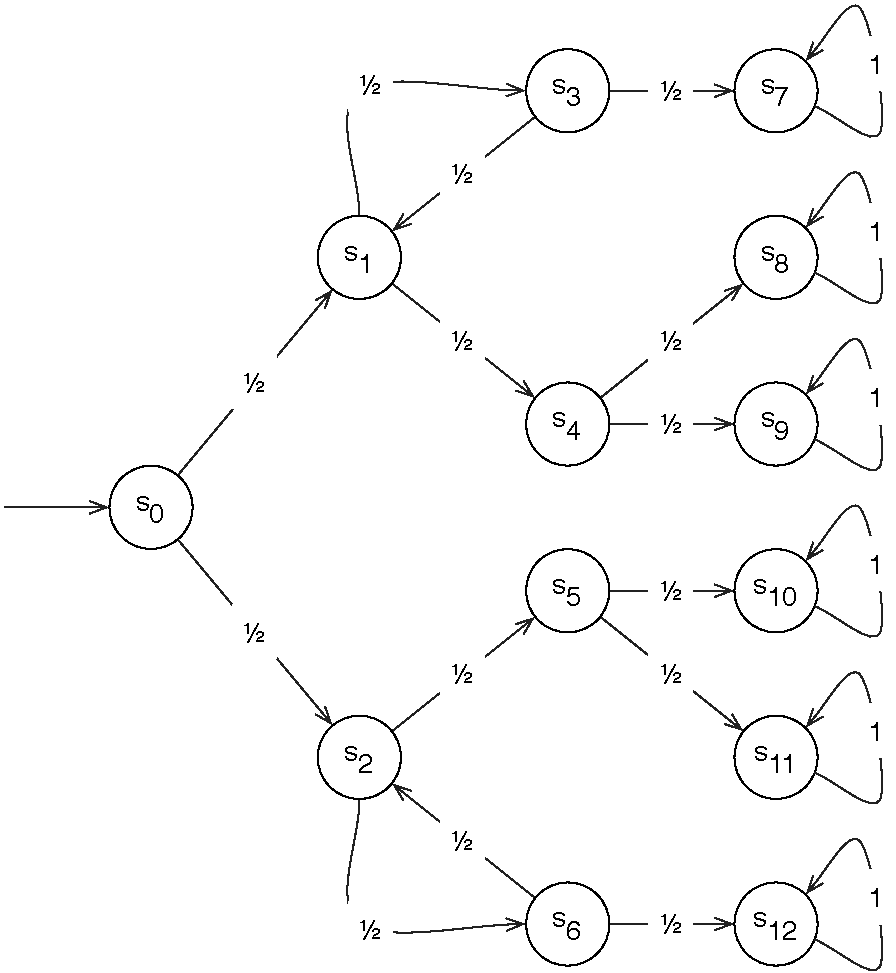
\includegraphics[scale=0.58]{img/example-DTMC.pdf}
\caption[A discrete-time Markov chain example]{The (discrete-time) Markov chain for a six-sided die simulated via a fair coin~\cite{Baier_2008}.}
\label{fig:example_DTMC}
\end{figure}

The DTMC in Figure~\ref{fig:example_DTMC} comprises an initial node $s_0$---such that $\iota_{init}(s_0) = 1$ and $\forall s \neq s_0: \iota_{init}(s) = 0$---and twelve states $S = \{s_1,\ldots,s_{12}\}$. Six inner states $\{s_1,\ldots,s_6\}$ and six terminating states $\{s_7,\ldots,s_{12}\}$ represent the tossing of a coin and possible die outcomes, repsectively. A Markov chain path, which can be rendered as a directed path in the underlying digraph, is a non-empty sequence of states $\pi = s_0\;s_1\;s_2 \cdots \in S^\omega$ such that $\forall i \ge 0: P(s_i, s_{i+1}) > 0$.

For a given DTMC, the transition probability function~$\mathbf{P}$ and the initial distribution $\iota_{init}$ can be represented, respectively, by a transition matrix $\left(\mathbf{P}(s, s')\right)_{s \in S}$ and an initial distribution vector $\left(\iota_{init}(s)\right)_{s \in S}$. The matrix specifies for each state $s \in S$ the probability $\mathbf{P}(s, s')$ of transitioning from~$s$ to~$s'$ in a discrete time-step. The vector specifies for each state $s \in S$ the probability $\iota_{init}(s)$ that the system evolution begins in~$s$. Figure~\ref{fig:transition_matrix_initial_distribution_vector} provides a partial transition matrix and a partial initial distribution vector for the DTMC in Figure~\ref{fig:example_DTMC}.

\setcounter{MaxMatrixCols}{11}

\begin{figure}[ht]
	\begin{equation*}
		\mathbf{P} =
			\begin{array}{c}
				\\
				s_0\\
				s_1\\
				s_2\\
				s_3\\
				s_4\\
				\vdots\\
			\end{array}
			\begin{array}{c}
				\begin{array}{
						c@{\hspace{0.9em}}
						c@{\hspace{0.9em}}
						c@{\hspace{0.9em}}
						c@{\hspace{0.9em}}
						c@{\hspace{0.9em}}
						c@{\hspace{0.9em}}
						c@{\hspace{0.9em}}
						c@{\hspace{0.9em}}
						c@{\hspace{0.9em}}
						c@{\hspace{0.9em}}
						c
					}
					s_0 & s_1 & s_2 & s_3 & s_4 & s_5 & s_6 & s_7 & s_8 & s_9 & \cdots\\
				\end{array}\\
				\left[
					\begin{array}{
							c@{\hspace{1.2em}}
							c@{\hspace{1.2em}}
							c@{\hspace{1.2em}}
							c@{\hspace{1.2em}}
							c@{\hspace{1.2em}}
							c@{\hspace{1.2em}}
							c@{\hspace{1.2em}}
							c@{\hspace{1.2em}}
							c@{\hspace{1.2em}}
							c@{\hspace{1.2em}}
							c
						}
						0 & \frac{1}{2} & \frac{1}{2} & 0 & 0 & 0 & 0 & 0 & 0 & 0 & \cdots\\
						0 & 0 & 0 & \frac{1}{2} & \frac{1}{2} & 0 & 0 & 0 & 0 & 0 & \cdots\\
						0 & 0 & 0 & 0 & 0 & \frac{1}{2} & \frac{1}{2} & 0 & 0 & 0 & \cdots\\
						0 & \frac{1}{2} & 0 & 0 & 0 & 0 & 0 & \frac{1}{2} & 0 & 0 & \cdots\\
						0 & 0 & 0 & 0 & 0 & 0 & 0 & 0 & \frac{1}{2} & \frac{1}{2} & \cdots\\
						\vdots & \vdots & \vdots & \vdots & \vdots & \vdots & \vdots & \vdots & \vdots & \vdots & \ddots\\
					\end{array}
				\right]
			\end{array}
		\iota_{init} =
			\begin{array}{c}
				\\
				s_0\\
				s_1\\
				s_2\\
				s_3\\
				s_4\\
				\vdots\\
			\end{array}
			\begin{array}{c}
				\begin{array}{c}
					\\
				\end{array}\\
				\left[
					\begin{array}{c}
						1\\
						0\\
						0\\
						0\\
						0\\
						\vdots\\
					\end{array}
				\right]
			\end{array}
	\end{equation*}
	\caption[Transition matrix and initial distribution vector examples]{The partial transition matrix and partial initial distribution vector for a six-sided die simulated via a fair coin, as illustrated in Figure~\ref{fig:example_DTMC}.}
	\label{fig:transition_matrix_initial_distribution_vector}
\end{figure}

Probabilistic model checking can be used to verify both quantitative and qualitative DTMC properties. The former constrain probabilities to specific thresholds, while the latter associate desirable and undesirable behavior with probabilities of one and zero, respectively. PCTL is an extension of the branching-time \emph{computation tree logic} (CTL), and a prominent formalism for expressing probabilistic properties. PCTL supports the probabilistic operator $\mathbb{P}_{J}(\varphi)$, where $\varphi$ specifies a constraint over the set of paths that constitute a Markov chain, and $J$ specifies a closed interval between one and zero that bounds the probability of satisfying $\varphi$.

\section{UAV Missions}
\label{sec:UAV_Missions}

UAVs, or \emph{uninhabited aerial systems} (UASs), are aircraft capable of either autonomous or remote controlled flight. Primarily oriented toward (dull, dirty and dangerous) military missions, UAVs are increasingly relied upon to perform agricultural, scientific, industrial and law-enforcement tasks over civilian airspace~\cite{Rango_2010,Jimenez_Berni_2009,Heintz_2007}.

The UAV domain exhibits complexity at different levels of granularity. UAVs incorporate sophisticated payloads, multiple sensors and increasing computational power. These capabilities could, in time, enable UAV swarms to execute complex multi-task missions with reduced human supervision~\cite{Karaman_2008}. Figure~\ref{fig:UAV_autonomy} illustrates various levels of UAV autonomy, ranging from remotely guided drones to fully autonomous swarms, which correspond to levels of automation originally proposed by Sheridan and Verplank~\cite{Nowak_2007}. For any given mission, autonomous UAVs may be required to execute tasks synchronously and in real-time; with local, incomplete and/or noisy knowledge; and in the context of a dynamic environment~\cite{Tosic_2003}. These factors combine to form a complex stochastic state space that motivates the probabilistic verification of UAV mission plans.

\begin{figure}[ht]
\centering
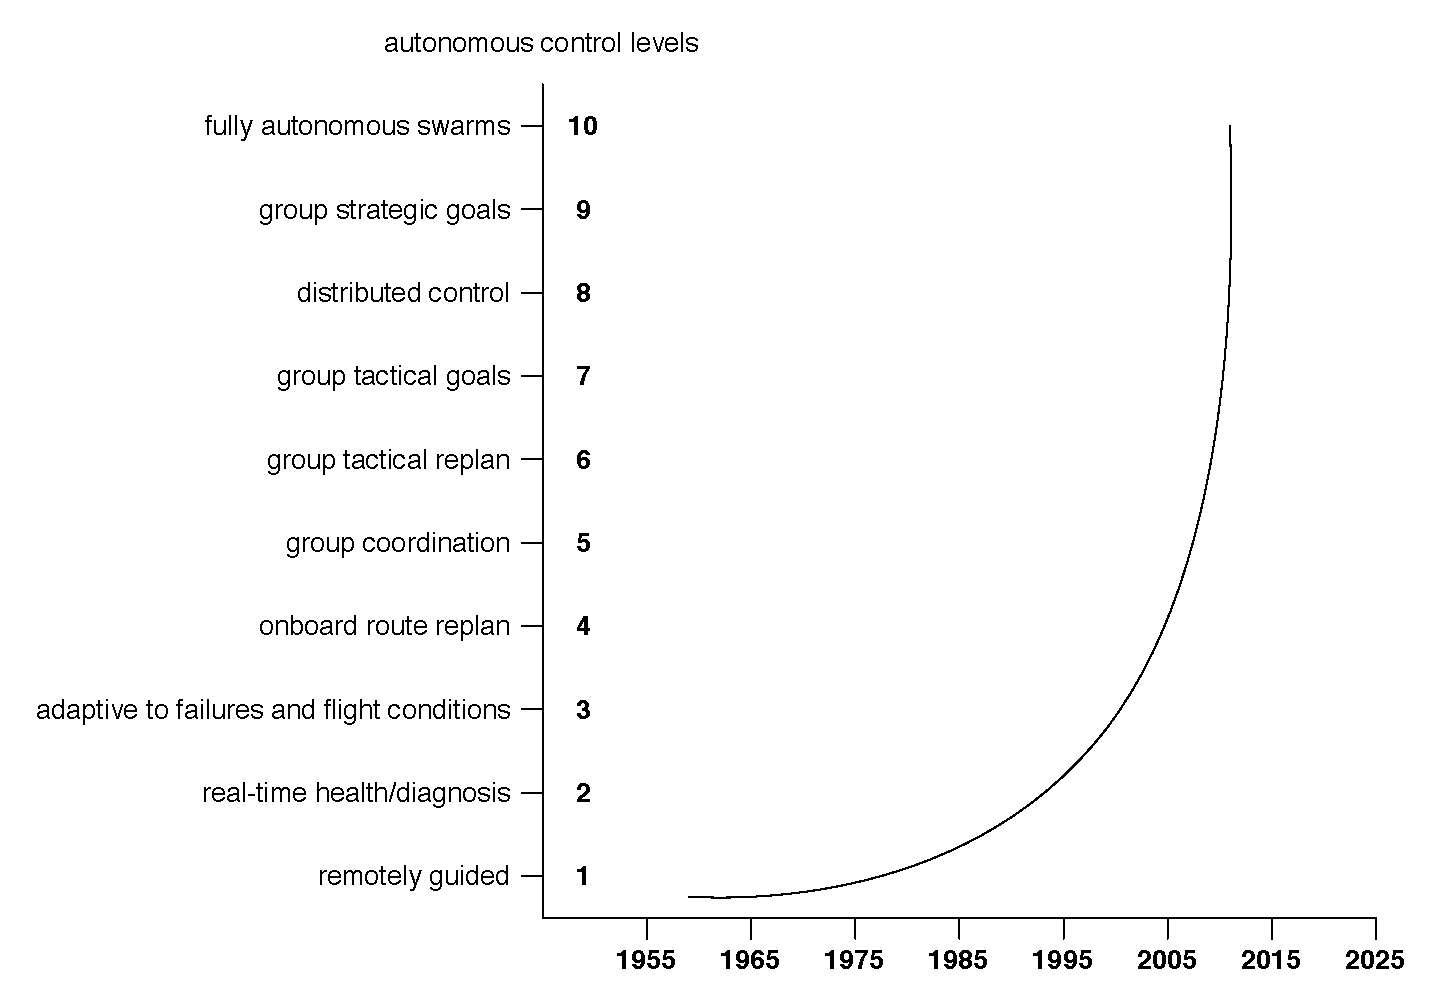
\includegraphics[scale=0.58]{img/UAV-autonomy.pdf}
\caption[UAV autonomy hierarchy]{A hierarchy of UAV autonomy levels~\cite{Youngson_2004,DoD_2005}.}
\label{fig:UAV_autonomy}
\end{figure}

This section provides a concise overview of what is an expansive application domain. Chapter~\ref{chap:Domain_Modeling} explores a subset of that domain in greater detail.

\subsection{UAV Performance Specifications}
\label{sec:UAV_Performance_Specifications}

UAVs can be classified with respect to their performance specifications, and the mission requirements that those specifications are meant to address~\cite{Arjomandi}. UAV performance specifications include the following:

\begin{itemize}

\item \emph{ceiling} (measured in meters), ``an aircraft's maximum pressure height''~\cite{Crocker_2007};

\item \emph{cost};

\item \emph{endurance} (hours), ``the length of time an aircraft can stay in the air without refueling''~\cite{Crocker_2007};

\item \emph{engine type};

\item \emph{payload} (kilograms), ``the load carried by an aircraft''~\cite{Crocker_2007};

\item \emph{power} (kilowatt), ``the propulsive power needed to produce thrust''~\cite{Crocker_2007};

\item \emph{range} (kilometers), ``the maximum distance an aircraft can fly on a given amount of fuel''~\cite{Crocker_2007};

\item \emph{speed} (kilometers per hour);

\item \emph{weight} (kilograms);

\item \emph{wing loading} ($\textrm{kg/m}^2$), ``the weight of an aircraft per unit wing area''~\cite{Crocker_2007};

\item \emph{wing span} (meters), ``a measurement from the tip of one wing to the tip of the other wing''~\cite{Crocker_2007}.

\end{itemize}

Table~\ref{tab:UAV_performance_specifications} lists the performance specifications for various active (at the time of writing) military- and commercial-grade UAVs~\cite{Arjomandi,AscTec,Draganfly,Parrot}. The range of values encompassed by each performance specification can be divided into categories~\cite{Arjomandi}. Table~\ref{tab:UAV_performance_specification_categories} uses these categories to classify a subset of the UAVs listed in Table~\ref{tab:UAV_performance_specifications}.

\begin{sidewaystable}
	\centering
	\arrayrulecolor{Gray}
	\renewcommand*\arraystretch{1.3}
	\begin{tabular}{ l l | c c c c c c c c c }
		\multirow{2}{*}{\emph{UAV}} &
			\multirow{2}{*}{\emph{manufacturer}} &
			\emph{ceiling} &
			\emph{endurance} &
			\emph{payload} &
			\emph{range} &
			\emph{speed} &
			\emph{weight} &
			\emph{wing loading} &
			\emph{wing span}\\
			& & (m) & (hr) & (kg) & (km) & (km/h) & (kg) & ($\textrm{kg/m}^2$) & (m)\\
		\hline
		BQM-147 Dragon & BAI Aerosystems & 3,048 & 3 & 11 & 148 & 160 & 41 & 22 & 2\\
		Crecerelle & SAGEM & 3,353 & 6 & 35 & 59 & 246 & 120 & 9 & 3\\
		Heron (Machatz-1) & Israel Aerospace Industries & 10,000 & 40 & 227 & 3,300 & 207 & 1,087 & 70 & 17\\
		Luna X-2000 & EMT Penzberg & 4,000 & 4 & 10 & 80 & 160 & 40 & 40 & 4\\
		MQ-1 Predator & General Atomics & 7,920 & 20 & 600 & 740 & 217 & 1,020 & 89 & 15\\
		MQ-8 Fire Scout & Northrop Grumman & 6,096 & 6 & 90 & 400 & 231 & 1,159 & 69 & 9\\
		MQ-9 Reaper & General Atomics & 15,200 & 24 & 3,000 & 1,500 & 405 & 4,500 & 83 & 20\\
		RQ-2 Pioneer & AAI Corporation & 4,572 & 5 & 64 & 373 & 175 & 125 & 34 & 5\\
		RQ-4 Global Hawk & Northrop Grumman & 20,000 & 30 & 900 & 22,000 & 636 & 11,600 & 199 & 35\\
		RQ-7 Shadow & AAI Corporation & 4,270 & 5 & 75 & 125 & 204 & 149 & 79 & 4\\
		RQ-11 Raven & AeroVironment & 4,267 & 4 & 17 & 100 & 204 & 84 & 57 & 3\\
		RQ-14 Dragon Eye & AeroVironment & 305 & 1 & 0 & 5 & 65 & 2 & 5 & 1\\
		RQ-15 Neptune & DRS Technologies & 2,440 & 4 & 10 & 75 & 156 & 36 & 74 & 2\\
		\hline
		AR.Drone 1.0 & Parrot & 6--50 & 0.2 & 0 & 0.05--0.335 & 18 & 0.38--0.42 & n/a & n/a\\
		Falcon 8 & AscTec & 2,500 & 0.27--0.3 & 0.5 & 0.15 & 10.8--54 & 0.8 & n/a & n/a\\
		X6 & Draganfly & 2,438 & n/a & 0.5 & n/a & 50 & 1 & n/a & n/a\\
	\end{tabular}
	\caption[UAV performance specifications]{Performance specifications for various military- and commercial-grade UAVs (top and bottom, respectively) including the established MQ-1 Predator and MQ-9 Reaper from General Atomics; and the MQ-8 Fire Scout helicopter from Northrop Grumman.}
	\label{tab:UAV_performance_specifications}
\end{sidewaystable}

\begin{table}[ht]
	\arrayrulecolor{Gray}
	\renewcommand*\arraystretch{1.3}
	\begin{tabularx}{\textwidth}{
			>{\centering\hsize=0.3\hsize}X|
			>{\centering\hsize=0.2\hsize}X|
			>{\centering\hsize=0.2\hsize}X|
			>{\centering\hsize=0.3\hsize}X
		}
		\emph{specification} &
			\emph{category} &
			\emph{range} &
			\emph{UAV}\tabularnewline
		\hline
		\multirow{3}{*}{\emph{ceiling} (m)}
			& low & $<$1000 & RQ-14 Dragon Eye\tabularnewline
			& medium & 1000--10,000 & MQ-1 Predator\tabularnewline
			& high & $>$10,000 & RQ-4 Global Hawk\tabularnewline
		\hline
		\multirow{3}{*}{\emph{endurance} (hr)}
			& low & $<$5 & RQ-14 Dragon Eye\tabularnewline
			& medium & 5--24 & MQ-1 Predator\tabularnewline
			& high & $>$24 & RQ-4 Global Hawk\tabularnewline
		\hline
		\multirow{3}{*}{\emph{range} (km)}
			& low & $<$100 & RQ-14 Dragon Eye\tabularnewline
			& medium & 100--1500 & MQ-1 Predator\tabularnewline
			& high & $>$1500 & RQ-4 Global Hawk\tabularnewline
		\hline
		\multirow{5}{*}{\emph{weight} (kg)}
			& micro & $<$5 & RQ-14 Dragon Eye\tabularnewline
			& light & 5--50 & RQ-15 Neptune\tabularnewline
			& medium & 50--200 & RQ-11 Raven\tabularnewline
			& heavy & 200--2000 & MQ-1 Predator\tabularnewline
			& super heavy & $>$2000 & RQ-4 Global Hawk\tabularnewline
		\hline
		\multirow{3}{*}{\emph{wing loading} ($\textrm{kg/m}^2$)}
			& low & $<$50 & RQ-14 Dragon Eye\tabularnewline
			& medium & 50--100 & MQ-1 Predator\tabularnewline
			& high & $>$100 & RQ-4 Global Hawk\tabularnewline
	\end{tabularx}
	\caption[UAV performance specification categories]{Performance specification categories with their respective ranges, and illustrative UAV classifications.}
	\label{tab:UAV_performance_specification_categories}
\end{table}

UAVs can also be classified with respect to the following mission aspects, which categorize mission requirements.

\begin{itemize}

\item \emph{Aerial delivery and resupply} requires UAVs to supply special forces teams covertly and precisely with small quantities of cargo including batteries, water and leaflets for psychological operations~\cite{DoD_2005}.

\item \emph{Combat} requires highly maneuverable \emph{unmanned combat aerial vehicles} (UCAVs) to engage in both air-to-air and air-to-surface combat~\cite{Arjomandi}.

\item \emph{Intelligence, surveillance, target acquisition and reconnaissance} (ISTAR) requires UAVs to enhance situational awareness by collecting battlefield information.

\item \emph{Multi-purpose} requires UAVs to conduct armed reconnaissance against critical and perishable targets.

\item \emph{Radar and communication relay} requires \emph{airborne communication nodes} (ACNs) to ensure information superiority by extending and enhancing tactical intra-theater communications~\cite{DoD_2005}.

\item \emph{Vertical take-off and landing} (VTOL) requires UAVs to generate sufficient downward thrust to takeoff, hover and land within very limited space.

\end{itemize}

The performance specification categories that classify each UAV address a particular set of mission aspects~\cite{Arjomandi}. For example, the MQ-1 Predator is classified as a medium altitude (1000--10,000 meters), medium endurance (5--24 hours), medium range (100--400 km) and heavy weight (200--2000 kg) UAV\@. These classifications determine the Predator to be highly-desirable for ISTAR and multi-purpose missions, and unsuitable for all remaining mission aspects. Table~\ref{tab:UAV_classifications} classifies the military-grade UAVs listed in Table~\ref{tab:UAV_performance_specifications} with a rating scale of zero to four, where zero indicates the inability of a UAV to perform a specific mission aspect; and values in the range of one to four indicate the degree of compatibility, from lowest to highest, respectively, between performance specifications that parameterize UAVs and the performance specifications required by mission aspects.

\begin{table}[ht]
	\arrayrulecolor{Gray}
	\renewcommand*\arraystretch{1.3}
	\begin{tabularx}{\textwidth}{
			>{\raggedright\hsize=0.29\hsize}X|
			>{\centering\hsize=0.13\hsize}X
			>{\centering\hsize=0.13\hsize}X
			>{\centering\hsize=0.13\hsize}X
			>{\centering\hsize=0.19\hsize}X
			>{\centering\hsize=0.13\hsize}X
		}
		& \emph{delivery} &
			\emph{UCAV} &
			\emph{ISTAR} &
			\emph{multi-purpose} &
			\emph{ACN}\tabularnewline
		\hline
		BQM-147 Dragon & 0 & 0 & 0 & 0 & 0\tabularnewline
		Crecerelle & 0 & 0 & 0 & 0 & 0\tabularnewline
		Heron (Machatz-1) & 0 & 0 & 3 & 0 & 0\tabularnewline
		Luna X-2000 & 0 & 0 & 1 & 0 & 0\tabularnewline
		MQ-1 Predator & 0 & 0 & 3 & 4 & 0\tabularnewline
		MQ-8 Fire Scout & 0 & 0 & 0 & 0 & 2\tabularnewline
		MQ-9 Reaper & 0 & 0 & 0 & 0 & 0\tabularnewline
		RQ-2 Pioneer & 0 & 0 & 1.5 & 0 & 0\tabularnewline
		RQ-4 Global Hawk & 0 & 0 & 4 & 0 & 0\tabularnewline
		RQ-7 Shadow & 0 & 0 & 1.5 & 0 & 0\tabularnewline
		RQ-11 Raven & 0 & 0 & 0 & 0 & 0\tabularnewline
		RQ-14 Dragon Eye & 0 & 0 & 1 & 0 & 0\tabularnewline
		RQ-15 Neptune & 0 & 0 & 1 & 0 & 0\tabularnewline
	\end{tabularx}
	\caption[UAV classifications]{UAV classifications with respect to the degree of compatibility between performance specifications that parameterize UAVs and the performance specifications required by (abbreviated) mission aspects. Compatibility is rated with a scale of zero to four, where zero indicates the inability of a UAV to perform a specific mission aspect.}
	\label{tab:UAV_classifications}
\end{table}

\subsection{UAV Mission Hierarchy}
\label{sec:UAV_Mission_Hierarchy}

We distinguish mission aspect from mission; the former is a conceptualization of related mission requirements, the latter a structured collection of interrelated tasks. Table~\ref{tab:mission_hierarchy} presents a tabular hierarchy of military and commercial UAV missions~\cite{Nehme_2006}. High-level missions, which correspond partially to the mission aspects presented in Section~\ref{sec:UAV_Performance_Specifications}, include the following:

\begin{itemize}

\item \emph{communication}, the relay of voice and data between units, and from units to a higher command;

\item \emph{drones}, the imitation of fighter aircraft or other objects for the purposes of training or (enemy) deception;

\item \emph{extraction}, the removal (including search and rescue) of personnel and cargo from a specified target;

\item \emph{insertion}, the delivery of lethal and non-lethal payloads (for example, emergency supplies) to a specified target;

\item \emph{intelligence}, the accumulation, analysis and dissemination of enemy, terrain and weather information in areas of interest or operation;

\item \emph{reconnaissance}, the exploration or inspection of a specific area for the purpose of information gathering;

\item \emph{surveillance}, the (often clandestine) monitoring of behavior and activities;

\item \emph{transport}, the movement or transfer of personnel and cargo between two locations.

\end{itemize}

\definecolor{E1E1E1}{RGB}{225,225,225}
\definecolor{F1F1F1}{RGB}{241,241,241}

\begin{table}[!ht]
	\arrayrulecolor{Gray}
	\renewcommand*\arraystretch{1.3}
	\begin{tabularx}{\textwidth}{ X | X | X }
		\emph{level 1} & \emph{level 2} & \emph{level 3}\\
		\hline
		\multicolumn{3}{ >{\columncolor{E1E1E1}}l }{drones}\\
		\hline
		& \multicolumn{2}{ >{\columncolor{F1F1F1}}l }{decoy}\\
		\hline
		& \multicolumn{2}{ >{\columncolor{F1F1F1}}l }{target practice}\\
		\hline
		\multicolumn{3}{ >{\columncolor{E1E1E1}}l }{communication}\\
		\hline
		\multicolumn{3}{ >{\columncolor{E1E1E1}}l }{extraction}\\
		\hline
		\multicolumn{3}{ >{\columncolor{E1E1E1}}l }{insertion}\\
		\hline
		& \multicolumn{2}{ >{\columncolor{F1F1F1}}l }{electronic warfare}\\
		\hline
		& & electronic attack\\
		\hline
		& & electronic protection\\
		\hline
		& \multicolumn{2}{ >{\columncolor{F1F1F1}}l }{payload delivery}\\
		\hline
		& & lethal\\
		\hline
		& & non-lethal\\
		\hline
		\multicolumn{3}{ >{\columncolor{E1E1E1}}l }{intelligence/reconnaissance}\\
		\hline
		& \multicolumn{2}{ >{\columncolor{F1F1F1}}l }{BDA}\\
		\hline
		& \multicolumn{2}{ >{\columncolor{F1F1F1}}l }{mapping}\\
		\hline
		& \multicolumn{2}{ >{\columncolor{F1F1F1}}l }{target acquisition}\\
		\hline
		& & dynamic target\\
		\hline
		& & static target\\
		\hline
		& \multicolumn{2}{ >{\columncolor{F1F1F1}}l }{target designation}\\
		\hline
		\multicolumn{3}{ >{\columncolor{E1E1E1}}l }{transport}\\
		\hline
		& \multicolumn{2}{ >{\columncolor{F1F1F1}}l }{cargo}\\
		\hline
		& \multicolumn{2}{ >{\columncolor{F1F1F1}}l }{passengers}\\
		\hline
		\multicolumn{3}{ >{\columncolor{E1E1E1}}l }{surveillance}\\
		\hline
		& \multicolumn{2}{ >{\columncolor{F1F1F1}}l }{geospatial surveillance}\\
		\hline
		& & dynamic target\\
		\hline
		& & static target\\
		\hline
		& \multicolumn{2}{ >{\columncolor{F1F1F1}}l }{listening}\\
		\hline
		& \multicolumn{2}{ >{\columncolor{F1F1F1}}l }{NBC sensing}\\
	\end{tabularx}
	\caption[UAV mission hierarchy]{A tabular UAV mission hierarchy, which includes \emph{battle damage assessment} (BDA) and \emph{nuclear, biological and chemical} (NBC) sensing missions.}
	\label{tab:mission_hierarchy}
\end{table}

Table~\ref{tab:mission_hierarchy} divides the \emph{intelligence, surveillance, and reconnaissance} (ISR) mission space, which is itself a subset of the ISTAR mission aspect, into \emph{intelligence/reconnaissance} and \emph{surveillance} missions. When considered from a different perspective, airborne ISR missions can also be divided into mutually exclusive mission segments including \emph{standoff}, which requires ISR platforms to respect the sovereign airspace of other nations; \emph{over flight}, which authorizes ISR platforms to perform low-risk violations of sovereign airspace, with or without consent from the nation whose airspace is being violated; and \emph{denied}, which exposes ISR platforms to a potentially hostile airspace~\cite{DoD_2005}.

UAV missions in general can be divided into planning, management, and re-planning segments to identify functions that will be assumed by human operators~\cite{Nehme_2006}. For example, drone mission segments comprise the following tasks:

\begin{itemize}

\item \emph{mission planning}, the use of 1) a scheduling mechanism to plan health and status reports, 2) threat area and no-fly zone information to designate the area of deployment, and 3) a decision support mechanism to designate loiter locations;

\item \emph{mission management}, the use of indicators to monitor the health, status and progress of a UAV;

\item \emph{mission re-planning}, the use of path planning to re-designate deployment areas.

\end{itemize}

Given these tasks, drone missions require human operators to supervise path planning, and to monitor the health and status of UAVs. Transport missions extend drone missions by requiring operators to monitor the health and status of passengers. Insertion missions, which are more demanding, require operators to supervise path planning; monitor the health and status of the UAV; monitor the status of weapons; identify targets; allocate and schedule resources; and negotiate with, and notify, other stakeholders. Nehme et al.\ provide a comprehensive discussion on UAV missions, and the function of human operators with respect to those missions~\cite{Nehme_2006}.

We have presented UAV missions from multiple perspectives, which support the analysis of mission scenarios at different levels of granularity (from high-level mission objectives with tactical and political implications to low-level tasks performed by human operators). Section~\ref{sec:DARPA_Mission_Scenario} and Section~\ref{sec:DRDC_Mission_Scenario} introduce two illustrative mission scenarios.

\subsection{DARPA Mission Scenario}
\label{sec:DARPA_Mission_Scenario}

UAVForge was a collaborative initiative by DARPA and the Space and Naval Warfare Systems Center Atlantic (SSC Atlantic)~\cite{DARPA}. The aim of the initiative was to crowd-source the design and development of a remotely operated micro-UAV that could be transported in a rucksack by a single person traveling on foot. Submitted UAVs were evaluated in the context of a mission scenario, which involved the observation of suspicious activities occurring in the vicinity of two nondescript urban buildings. Total mission time did not exceed five and a half hours including three hours for the observation task. UAVs were required to demonstrate the following capabilities:

\begin{itemize}

\item vertical take-off(s) from, and landing(s) to, different stationary locations;

\item safe flight within an altitude window of 5--1000 feet, with up to 15 mile per hour winds and 40--100\textdegree F temperatures;

\item point-to-point navigation within 500 feet of defined flight corridors;

\item operation within an assigned airspace and avoidance of defined no-fly zones;

\item (preferably autonomous) avoidance of static and (potentially) dynamic obstacles---including buildings, water towers, and trees---during approach into an observation area;

\item landing in an area similar to a rooftop structure containing \emph{heating, ventilation, and air conditioning} (HVAC) equipment, communications gear, satellite dishes and poles;

\item identification of a vantage point---up to 2.0 miles beyond line-of-sight from the starting location---from which to conduct the observation task

\item observation by landing on, adhering to, hanging over, and/or hovering above or below physical structures;

\item real-time transmission of images or video depicting static and mobile items of interest located up to 100 feet from the observing UAV;

\item data link frequency management and data transmission in compliance with rules and authorized frequencies stipulated, respectively, by the Academy of Model Aeronautics (AMA) and the U.S. Federal Communications Commission (FCC).

\end{itemize}

Figure~\ref{fig:UAVForge_competition_course} illustrates the UAVForge mission scenario, which underpins, and thereby lends credibility to, the~58 UAV mission plans developed for this project. These plans in turn support the development and evaluation of our method and prototype.

\begin{sidewaysfigure}
\centering
\includegraphics[scale=1]{img/UAVForge-competition-course.png}
\caption[DARPA's UAVForge mission scenario]{An illustration of DARPA's UAVForge mission scenario~\cite{DARPA}.}
\label{fig:UAVForge_competition_course}
\end{sidewaysfigure}

\subsection{DRDC Mission Scenario}
\label{sec:DRDC_Mission_Scenario}

The DRDC produces mission scenarios to further knowledge on the intersection of UAV/UCAV devices and \emph{intelligent adaptive interfaces} (IAIs), which are technologies for enhancing performance in complex socio-technical environments such as multi-UAV operations~\cite{Hou_2006,Hou_2011}. Mission scenarios employ a suite of UAV platforms---including \emph{medium altitude long endurance} (MALE) UAVs (for example, the MQ-1 Predator\footnote{In contrast to Youngson et al., Arjomandi classifies the MQ-1 Predator as a medium endurance UAV (see Table~\ref{tab:UAV_performance_specification_categories}).}), VTOL Tactical UAVs (VTUAVs), and mini UAVs---to evaluate the impact of IAI constructs on operations within the UAV domain in Canada~\cite{Youngson_2004}. We will focus on a mission scenario involving a \emph{fishery patrol} (FISHPAT) and a \emph{counter-drug operation} (CD OP), which are representative of domestic ISR missions undertaken by Canadian Forces in peacetime (additional domestic operations include disaster recovery, homeland security, long-duration law enforcement surveillance, and search and rescue).

The CD OP is coordinated from the Maritime Forces Atlantic (MARLANT) Headquarters at Canadian Forces Base (CFB) Halifax with support from HMCS Winnipeg. A \emph{ship of interest} (SOI) is initially tracked by US Customs aircraft and a US Coast Guard vessel. In conjunction with this activity, HMCS Montreal, which carries four VTUAVs, is conducting a FISHPAT approximately 180 nautical miles south of Burin in Newfoundland; and HMCS Kingston, which carries two mini UAVs, is conducting a coastal patrol 150 nautical miles southwest of Burin. Mission correctness is complicated by several factors. Tasked assets operate remotely and at great distances from their home bases. Extended transit times and accurate, timely intelligence reports are therefore critical to mission planning, and asset positioning and availability. In addition, the \emph{area of operation} (AOO) experiences weather conditions---including frequent and extensive fog, low cloud cover and precipitation---that limit the utility of \emph{electro-optical} (EO) and \emph{infrared} (IR) sensors.

A timeline of major mission events is divided into seven segments, which are deemed conducive to IAI experimentation. These segments identify periods of excessive operator workload resulting from ``the simultaneous receipt of sensor data \ldots\ [transmitted by] multiple UAVs; dynamic re-tasking of UAVs; transfer of UAV control between agencies; and concurrent control of multiple UAVs.''~\cite{Youngson_2004} Mission segments include the following (all times are Eastern Standard):

{
\parindent=0em
\parskip=\medskipamount

\newcommand{\myindent}[1]{\hangindent=2em\textbf{#1}}

\myindent{0210--0232 hrs}: HMCS Montreal and Viper~01 (a MALE UAV) are re-tasked from a FISHPAT and a training exercise, respectively, to the CD OP\@. Viper~01 is vectored into position by a \emph{mission control element} (MCE) located at CFB Greenwood. Alpha 51, a manned patrol aircraft, is also re-tasked from a training exercise in order to track the SOI\@.

\myindent{0325--0702 hrs}: HMCS Montreal maintains simultaneous control of two VTUAVs (Bingo~61 and Bingo~62) and receives \emph{synthetic aperture radar} (SAR) imagery from Viper~01.

\myindent{0750--0812 hrs}: Ship board and airborne MCEs---for example, HMCS Kingston and Alpha~52, respectively---execute multiple UAV payload (i.e., EO, IR, and SAR) control transfers.

\myindent{1110--1140 hrs}: Alpha~52 controls, dynamically re-tasks and monitors sensor data from two UAVs (Mike~91 and Mike~92) while receiving SAR imagery from Viper~01. This involves Alpha~52 launching Mike~91, and assuming control of Mike~92 from HMCS Kingston.

\myindent{1200--1432 hrs}: HMCS Montreal controls and monitors sensor data from three UAVs (Bingo~63, Bingo~64 and Mike~92) while receiving SAR imagery from Viper~01. This involves HMCS Montreal launching Bingo~64 to replace Bingo~63, and assuming control of Mike~92 from Alpha~52.

\myindent{1440--1525 hrs}: Alpha~52, HMCS Kingston and HMCS Montreal transfer control of UAVs in conjunction with the surveillance of multiple targets.

\myindent{1620--1700 hrs}: UAV sensor operations and frequency of reporting accelerate in response to an increased operational tempo.

}

As with UAVForge, the DRDC scenario underpins mission plans that in turn support the development and evaluation of our method and prototype.

\section{Summary}
\label{sec:Background_Summary}

This chapter presents background material on the technologies that constitute cascading verification. We also provide a broad, concise overview of the UAV domain to contextualize, and convey the inherent complexity of, UAV missions. Some of the information in this overview is never exploited by our work; for example, our prototype implementation of cascading verification does not incorporate the performance specifications and mission hierarchy presented in Section~\ref{sec:UAV_Performance_Specifications} and Section~\ref{sec:UAV_Mission_Hierarchy}, respectively. But this information is nevertheless pertinent because it has informed our research and development efforts. The scope of our prototype with respect to its application domain will be elaborated in subsequent chapters.

\chapter{Method Overview}
\label{chap:Method_Overview}

Figure~\ref{fig:method_and_prototype_schematic} illustrates a high-level, domain-agnostic schematic of our method and prototype. Domain experts, who are the method's primary stakeholders, use OWL to define domain concepts and their relationships; SWRL and Prolog to define rules; and PRISM's modeling and property specification languages to define, respectively, DTMC and PCTL templates. Model builders, who are also primary stakeholders, use a high-level DSL to encode system specifications for model checking. We note that domain knowledge is formalized once and subsequently reused to support the verification of multiple system specifications.

\begin{figure}[ht]
\centering
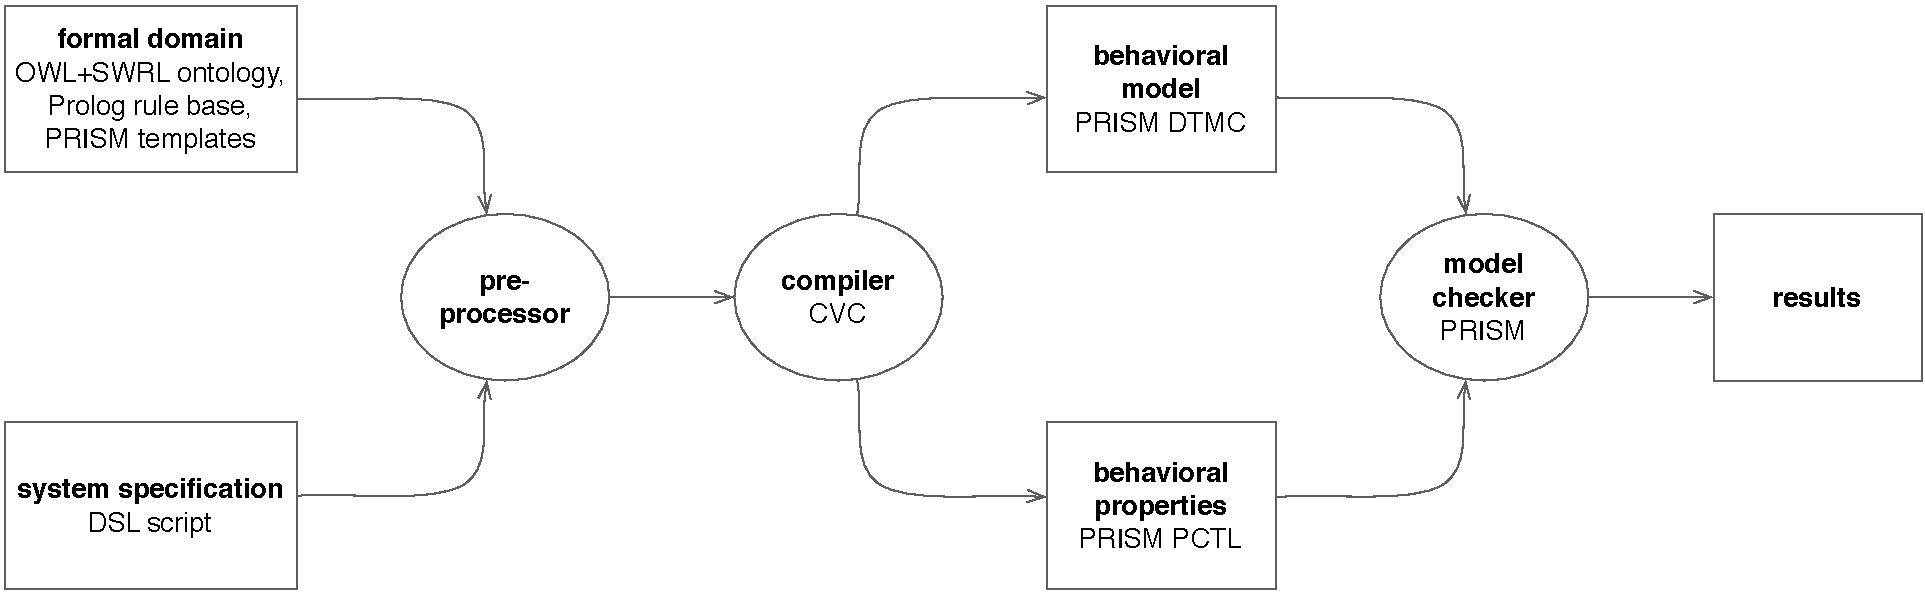
\includegraphics[width=\textwidth]{img/schematic.pdf}
\caption[Method and prototype schematic]{A high-level, domain-agnostic schematic of our method and prototype. Rectangular and oval shapes represent data and processes, respectively; and bold and normal text distinguishes method from prototype, respectively.}
\label{fig:method_and_prototype_schematic}
\end{figure}

\section{An Example Mission}
\label{sec:An_Example_Mission}

With our prototype, model builders use a domain-specific YAML dialect to encode mission plans comprising UAV \emph{assets} and the \emph{action workflows} assigned to those assets. The YAML code in Listing~\ref{lst:Mission_A} specifies Mission~A, an example mission that is representative of the~58 mission plans developed for this project.

\begin{figure}[ht]
\begin{lstlisting}[caption={YAML code for Mission~A},label=lst:Mission_A]
Action:
  TraversePathSegmentAction:
    - id: TPSA1
      duration: 60
      coordinates: [-118.27017, 34.04572,
        -118.27279, 34.04284]
    - id: TPSA2
      duration: 60
      coordinates: [-118.2739, 34.03928]
      preconditions: [TPSA1, TPSA3]
    - id: TPSA3
      duration: 60
      coordinates: [-118.26482, 34.03332,
        -118.27383, 34.03824]
    - id: TPSA4
      duration: 60
      coordinates: [-118.28204, 34.0376]
      preconditions: [TPSA3]
  PhotoSurveillanceAction:
    - id: PSA5
      duration: 50
      preconditions: [TPSA3]
Asset:
  Hummingbird:
    - id: H1
      actions: [TPSA1, TPSA2]
    - id: H2
      actions: [TPSA3, TPSA4, PSA5]
\end{lstlisting}
\end{figure}

Mission~A, which is illustrated in Figure~\ref{fig:example_mission}, comprises two \emph{Hummingbird} assets (lines~24--28 in Listing~\ref{lst:Mission_A}); a single \emph{photo surveillance action} (lines~19--22), which is a type of \emph{sensor action}; and four \emph{path segment traversal actions} (lines~2--18), which are \emph{kinetic actions}. A path segment traversal action instructs the executing UAV to traverse a path between two waypoints. For each such action, the latitudes and longitudes of the delineating waypoints are stored in an array and indexed in succession; in other words, the latitude of waypoint one is followed by the longitude of waypoint one, which is in turn followed by the latitude of waypoint two, etc. We note that the end coordinates of an action~\emph{a} constitute the start coordinates of an action~\emph{b} if~\emph{a} precedes~\emph{b}, and both~\emph{a} and~\emph{b} are assigned to the same asset; for example, the end coordinates of action \texttt{TPSA1} (line~6) constitute the implied start coordinates of action \texttt{TPSA2}, which succeeds \texttt{TPSA1} in the sequence of kinetic actions assigned to asset \texttt{H1} (line~26).

\begin{figure}[ht]
\centering
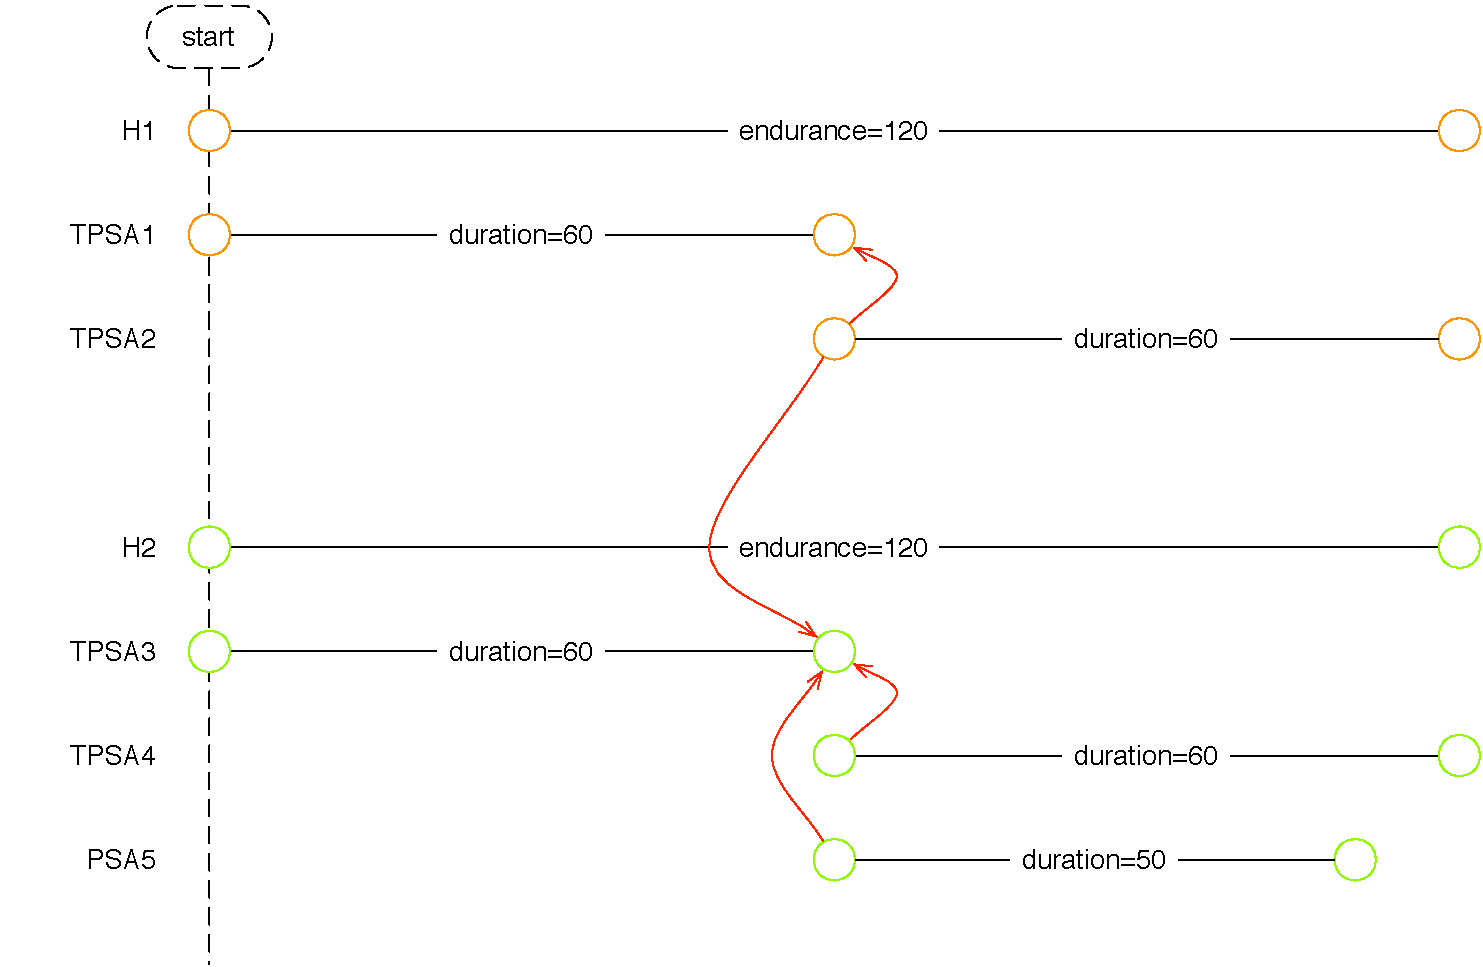
\includegraphics[scale=0.58]{img/example-mission.pdf}
\caption[A UAV mission example]{An illustration of Mission~A, with red arrows representing action dependencies and horizontal lines representing the passage of time. Color coded circles delineate the operation and execution of assets and actions, respectively, and group actions and the assets to which those actions are assigned.}
\label{fig:example_mission}
\end{figure}

With the exception of asset endurance, mission concepts specified in Listing~\ref{lst:Mission_A} correspond directly to the elements illustrated in Figure~\ref{fig:example_mission}. Asset endurance can be optionally omitted from mission specifications, and was therefore omitted for assets \texttt{H1} and \texttt{H2} in Mission~A, because the default endurance for Hummingbird assets is specified in an OWL+SWRL ontology, which will be presented in Chapter~\ref{chap:Domain_Modeling}. The following section describes the mechanism that integrates mission specifications with ontological knowledge.

\section{From Specification to Verification}
\label{sec:From_Specification_to_Verification}

For any given mission specification, a \emph{cascading verification compiler} (CVC) synthesizes both the DTMC and PCTL artifacts corresponding to that specification. Artifacts are synthesized as follows:

\begin{enumerate}

\item Mission specifications encoded in YAML are transformed by the CVC into ABox assertions. During this preprocessing phase, the CVC uses geographic coordinates from mission specifications, and data (pertaining to operational environments) from external sources, to perform geodetic calculations.\footnote{Geodetics is a branch of applied mathematics that deals with the size and shape of the Earth.} The equations that support these calculations are hard-coded in the CVC; for example, the compiler comprises geodesic equations that establish the occurrence, and calculate the duration, of threat area incursions committed by UAVs (these equations will be presented in Appendix~\ref{chap:Threat_Area_Calculations}). Geographic information resulting from preprocessing is integrated with the generated ABox.

\item We use Pellet, a sound and complete semantic reasoner~\cite{Sirin_2007}, to verify the generated ABox against the TBox defined by domain experts. In doing so, the reasoner ensures that mission constructs encoded in YAML are consistent with OWL+SWRL axioms. Inconsistencies between TBox and ABox signify an invalid mission specification, which causes the compilation process to terminate with an error. If consistency is deduced, then the reasoner proceeds to generate inferences from explicitly encoded domain knowledge; for example, if geodetic calculations establish the occurrence of a threat area incursion, then the asset committing that incursion is inferred to be a \emph{threatened asset}.

\item Inferred ontological knowledge is transformed by the CVC into Prolog facts. The compiler for SWI-Prolog---an open source implementation of Prolog~\cite{SWI_Prolog}---inputs the generated fact-base, and the Prolog rule-base defined by domain experts, and proceeds to generate inferences; for example, the last kinetic action in an action workflow is inferred to be a \emph{default terminal action}. The CVC uses Prolog inferences, in conjunction with explicit and inferred ontological knowledge, to synthesize DTMC and PCTL artifacts from predefined templates.

\end{enumerate}

PRISM inputs the synthesized artifacts, verifies the system model against its desired behavioral properties, and returns logical and probabilistic results from the verification. If the results are deemed acceptable by the model builder(s), then the mission can be scheduled for real-world execution (via some process that is outside the scope of our method).

In summary, cascading verification is a formal method that abstracts model checking for specific application domains. For a given domain of interest, experts in that domain implement a bespoke CVC once; and model builders use the implemented CVC to easily verify multiple system specifications.

We proceed to elaborate a subset of the UAV domain, which encompasses the concepts that constitute Mission~A.

\chapter{Domain Modeling}
\label{chap:Domain_Modeling}

This chapter describes the process of encoding domain knowledge in OWL+SWRL, Prolog, and DTMC and PCTL templates. The application of these technologies is illustrated with respect to the UAV domain and, in particular, Mission~A, the example mission presented in Section~\ref{sec:An_Example_Mission}.

The remainder of this chapter is structured as follows. Section~\ref{sec:Semantic_Modeling} uses OWL to formalize a subset of the UAV domain. The discussion is contextualized by case studies involving tactical and traffic surveillance missions, which are presented in Section~\ref{sec:Modeling_Tactical_Missions} and Section~\ref{sec:Modeling_Traffic_Surveillance_Missions}, respectively. Section~\ref{sec:Rule_Based_Modeling} uses SWRL to integrate complex relational structures into OWL, and Prolog to encode knowledge that can support effective reasoning with negation. Section~\ref{sec:Behavioral_Modeling} uses DTMC and PCTL formalisms to encode, respectively, probabilistic behavior and properties. DTMC and PCTL code is abstracted and presented in templates that support the synthesis of PRISM artifacts. Section~\ref{sec:Domain_Modeling_Related_Work} and Section~\ref{sec:Domain_Modeling_Summary} present related work and a summary of this chapter, respectively.

\section{Semantic Modeling}
\label{sec:Semantic_Modeling}

With cascading verification, domain experts use OWL+SWRL ontologies to formally define domain concepts and their relationships. For our prototype, we have developed a \emph{complex missions ontology} (CEMO) that formalizes a subset of the UAV domain. Domain concepts are integrated into a modular ontology architecture that supports flexible development and reuse~\cite{Bao_2006,Staab_2009}. The ontology development process utilized prominent Semantic Web technologies including the Prot\'{e}g\'{e} ontology editor, the Pellet reasoner and the Semantic Web Stack, which comprises OWL+SWRL\@.

\subsection{Building an OWL Ontology}
\label{sec:Building_an_OWL_Ontology}

Figure~\ref{fig:complex_missions_ontology} illustrates CEMO's class hierarchy, where each OWL class represents a grouping of individuals with similar characteristics~\cite{Bechhofer_2004}. Five classes---\texttt{Action}, \texttt{Area}, \texttt{Asset}, \texttt{Mission} and \texttt{Waypoint}---inherit directly from the built-in OWL class \texttt{Thing}, which represents the set of all individuals. (The built-in OWL class \texttt{Nothing} represents the empty set.) These concepts are accessible to all ontology modules that extend CEMO\@.

\begin{figure}[ht]
\centering
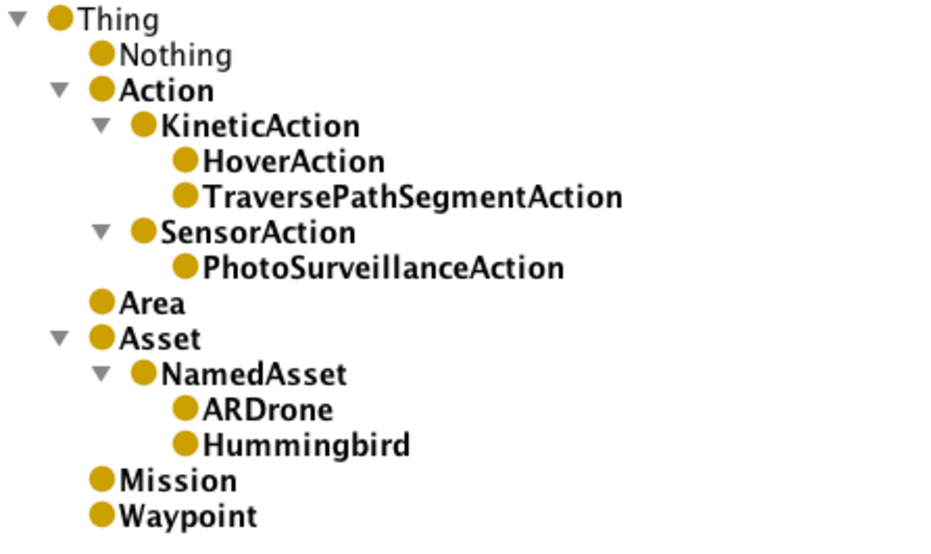
\includegraphics[scale=0.63]{img/cemo.pdf}
\caption[CEMO's class hierarchy]{CEMO's class hierarchy as presented by the Prot\'eg\'e ontology editor.}
\label{fig:complex_missions_ontology}
\end{figure}

The OWL code in Listing~\ref{lst:OWL_class_Asset} uses \emph{Manchester OWL syntax}---a human-friendly ontology representation language~\cite{Horridge_2006}---to formally defines class \texttt{Asset}, which is comprised in Mission~A\@. Lines~2--5 specify four OWL properties, which are constructs for describing relationships. In particular, an OWL property with specified \emph{domain} and \emph{range} links individuals from the domain to individuals or data values from the range. The two main OWL property types are \emph{object properties} and \emph{datatype properties}. The former describe relationships between two individuals while the latter describe relationships between individuals and data values.

\begin{lstlisting}[caption={OWL code for class \texttt{Asset}},label=lst:OWL_class_Asset]
Class: Asset
  SubClassOf: hasAction some KineticAction,
    hasCostValue some xsd:integer,
    hasEnduranceInSeconds some xsd:integer,
    hasSpeedInKilometersPerHour some xsd:integer
\end{lstlisting}

Lines~1 and~2 in Listing~\ref{lst:OWL_class_Asset} specify that every member of class \texttt{Asset} (the domain) must be associated with a member of class \texttt{KineticAction} (the range) via an instance of the object property \texttt{hasAction}. (For brevity, the reminder of this thesis will refer to \emph{property instances} simply as properties.) Members of class \texttt{Asset} are also associated with datatype properties describing asset cost, endurance and speed (lines~3--5).

Class \texttt{Asset} is extended by class \texttt{NamedAsset}, which is in turn extended by classes \texttt{ARDrone} and \texttt{Hummingbird}. The latter classes represent quadcopter UAVs manufactured by \href{http://ardrone2.parrot.com/usa/}{Parrot USA} and \href{http://www.asctec.de/}{Ascending Technologies}, respectively, that have informed our research. The OWL code in Listing~\ref{lst:OWL_class_Hummingbird} formally defines class \texttt{Hummingbird}, which is comprised in Mission~A\@.

\begin{figure}[ht]
\begin{lstlisting}[caption={OWL code for class \texttt{Hummingbird}},label=lst:OWL_class_Hummingbird]
Class: Hummingbird
  SubClassOf: NamedAsset,
    hasCostValue some xsd:integer[>= 5000],
    hasEnduranceInSeconds some xsd:integer[<= 120],
    hasSpeedInKilometersPerHour some xsd:integer[<= 50]
  DisjointWith: ARDrone
\end{lstlisting}
\end{figure}

Lines~3--5 in Listing~\ref{lst:OWL_class_Hummingbird} associate members of class \texttt{Hummingbird} with three datatype properties---\texttt{hasCostValue}, \texttt{hasEnduranceInSeconds} and \texttt{hasSpeedInKilometersPer\-Hour}. These properties are inherited from classes \texttt{NamedAsset} and, ultimately, \texttt{Asset}. Unlike class \texttt{Asset}, the ranges of the datatype properties that parameterize members of class \texttt{Hummingbird} restrict possible data values. Line~6 specifies that classes \texttt{ARDrone} and \texttt{Hummingbird} constitute \emph{disjoint} sets of individuals. Consequently, and appropriately, a member of class \texttt{ARDrone} cannot also be a member of class \texttt{Hummingbird}.

During a mission, assets execute actions that may be associated with other actions via \emph{preconditions}. An action~\emph{a} is a precondition to an action~\emph{b} if the end of~\emph{a} must precede the beginning of~\emph{b} in the sequence of actions that constitute an action workflow. Mission~A comprises three preconditions (lines~10, 18 and~22 in Listing~\ref{lst:Mission_A}), where each precondition relates actions assigned to the same asset. A fourth precondition (line~10) associates action \texttt{TPSA2} with action \texttt{TPSA3}, thereby coupling the behavior of the assets to which those actions are assigned (\texttt{H1} and~\texttt{H2}, respectively). CEMO encodes preconditions with the object property \texttt{hasPrecondition}, which is formally defined in Listing~\ref{lst:OWL_object_property_hasPrecondition}.

\begin{lstlisting}[caption={OWL code for the object property \texttt{hasPrecondition}},label=lst:OWL_object_property_hasPrecondition]
ObjectProperty: hasPrecondition
  Characteristics: Transitive
  Domain: Action
  Range: Action
  InverseOf: isPreconditionTo
\end{lstlisting}

Line~2 in Listing~\ref{lst:OWL_object_property_hasPrecondition} declares the object property \texttt{hasPrecondition} to be \emph{transitive}. Transitivity is one of several \emph{property characteristics} that can be used to qualify object properties. Given transitivity, if an action~\emph{a} is related via \texttt{hasPrecondition} to an action~\emph{b}, and~\emph{b} is related to an action~\emph{c} via the same property, then we can infer that~\emph{a} is related via \texttt{hasPrecondition} to~\emph{c}. In addition, \texttt{hasPrecondition} is inverted by the object property \texttt{isPreconditionTo} (line~5). The inverse relation between \texttt{hasPrecondition} and \texttt{isPreconditionTo} implies that if an action~\emph{a} is related via \texttt{hasPrecondition} to an action~\emph{b}, then~\emph{b} is related to~\emph{a} via \texttt{isPreconditionTo}. Figure~\ref{fig:transitive_properties} and Figure~\ref{fig:inverse_properties} illustrate transitivity and inversion, respectively.

\begin{figure}[ht]
\centering
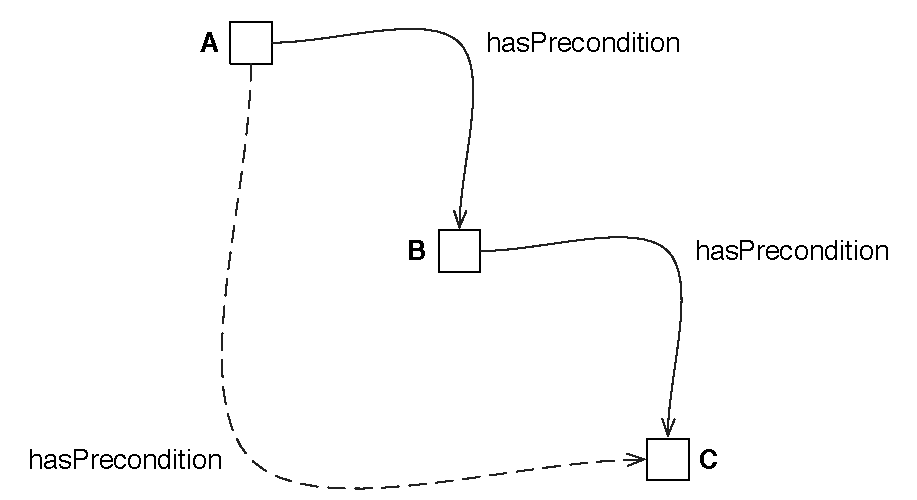
\includegraphics[scale=0.58]{img/transitive-properties.pdf}
\caption[Transitive properties]{An example of the transitive property characteristic that qualifies the object property \texttt{hasPrecondition}. The dashed line represents an inferred relationship.}
\label{fig:transitive_properties}
\end{figure}

\begin{figure}[ht]
\centering
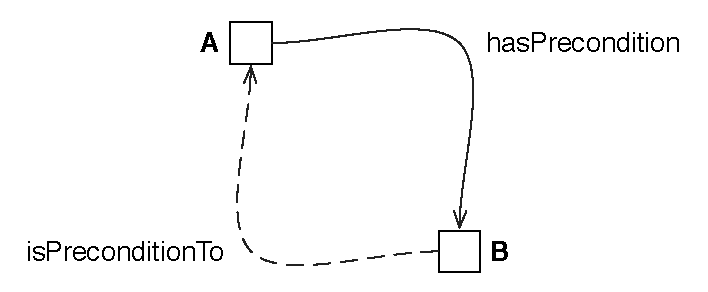
\includegraphics[scale=0.58]{img/inverse-properties.pdf}
\caption[Inverse properties]{An example of inversion with respect to the object properties \texttt{hasPrecondition} and \texttt{isPreconditionTo}. The dashed line represents an inferred relationship.}
\label{fig:inverse_properties}
\end{figure}

Because preconditions associate actions with other actions, class \texttt{Action} constitutes both the domain and range of the object property \texttt{hasPrecondition} (lines~3 and~4, respectively, in Listing~\ref{lst:OWL_object_property_hasPrecondition}). Class \texttt{Action} is extended by class \texttt{KineticAction}, whose members are associated with a data property describing action duration. Class \texttt{KineticAction} is in turn extended by classes \texttt{HoverAction} and \texttt{TraversePathSegment\-Action}. The OWL code in Listing~\ref{lst:OWL_class_TraversePathSegmentAction} formally defines class \texttt{TraversePathSegment\-Action}, which is comprised in Mission~A\@. Lines~3--4 in Listing~\ref{lst:OWL_class_TraversePathSegmentAction} specify that every member of class \texttt{TraversePathSegmentAction} must be associated via the object properties \texttt{hasStartPoint} and \texttt{hasEndpoint} with \texttt{Waypoint} individuals that designate the geographical start points and endpoints, respectively, of path segment traversal actions (hover actions are also designated geographically by waypoints).

\begin{lstlisting}[caption={OWL code for class \texttt{TraversePathSegmentAction}},label=lst:OWL_class_TraversePathSegmentAction]
Class: TraversePathSegmentAction
  SubClassOf: KineticAction,
    hasStartPoint some Waypoint,
    hasEndpoint some Waypoint
  DisjointWith: HoverAction
\end{lstlisting}

Class \texttt{Action} is also extended by class \texttt{SensorAction}, which is in turn extended by class \texttt{PhotoSurveillanceAction}. The OWL code in Listing~\ref{lst:OWL_class_PhotoSurveillanceAction} formally defines class \texttt{PhotoSurveillanceAction}, which is comprised in Mission~A\@.

\begin{lstlisting}[caption={OWL code for class \texttt{PhotoSurveillanceAction}},label=lst:OWL_class_PhotoSurveillanceAction]
Class: PhotoSurveillanceAction
  SubClassOf: SensorAction,
    hasDurationInSeconds some xsd:integer,
    hasPrecondition only Action
\end{lstlisting}

The preceding code contains the keywords \emph{some} (line~3) and \emph{only} (line~4), which represent, respectively, existential and universal restrictions in OWL\@. With regard to object properties:

\begin{itemize}

\item Existential restrictions describe classes of individuals that must participate in at least one relationship, along a specified property, with individuals that are members of a specified class~\cite{Horridge_2011}.

\item Universal restrictions describe classes of individuals that may, and can only, participate in relationships along a specified property with individuals that are members of a specified class.

\end{itemize}

\noindent Existential and universal restrictions, which can also be applied to datatype properties, are denoted in predicate logic by the existential ($\exists$) and universal ($\forall$) quantifiers, respectively.

\subsection{Modeling Tactical Missions}
\label{sec:Modeling_Tactical_Missions}

During tactical missions, assets may be required to commit threat area incursions, thereby compelling mission developers to consider the impact of asset \emph{survivability} on the probability of mission success. The United States Department of Defense (USDOD) defines survivability as ``the capability of a system \ldots\ to avoid or withstand a man-made hostile environment without suffering an abortive impairment in its ability to accomplish its designated mission.''~\cite{DoD_2001} To accommodate tactical mission requirements, we have developed a \emph{complex tactical missions ontology} (Tactical-CEMO) that extends CEMO\@.

Figure~\ref{fig:tactical_CEMO} illustrates Tactical-CEMO's multiple inheritance class hierarchy; for example, class \texttt{DirectThreatAreaHoverAction} extends classes \texttt{HoverAction} and \texttt{Threat\-AreaAction}. Classes describing tactical missions are highlighted in bold and thereby differentiate from classes encoded in CEMO\@. Used exclusively to support automated reasoning, tactical concepts are not available to mission developers via the YAML DSL\@.

\begin{figure}[ht]
\centering
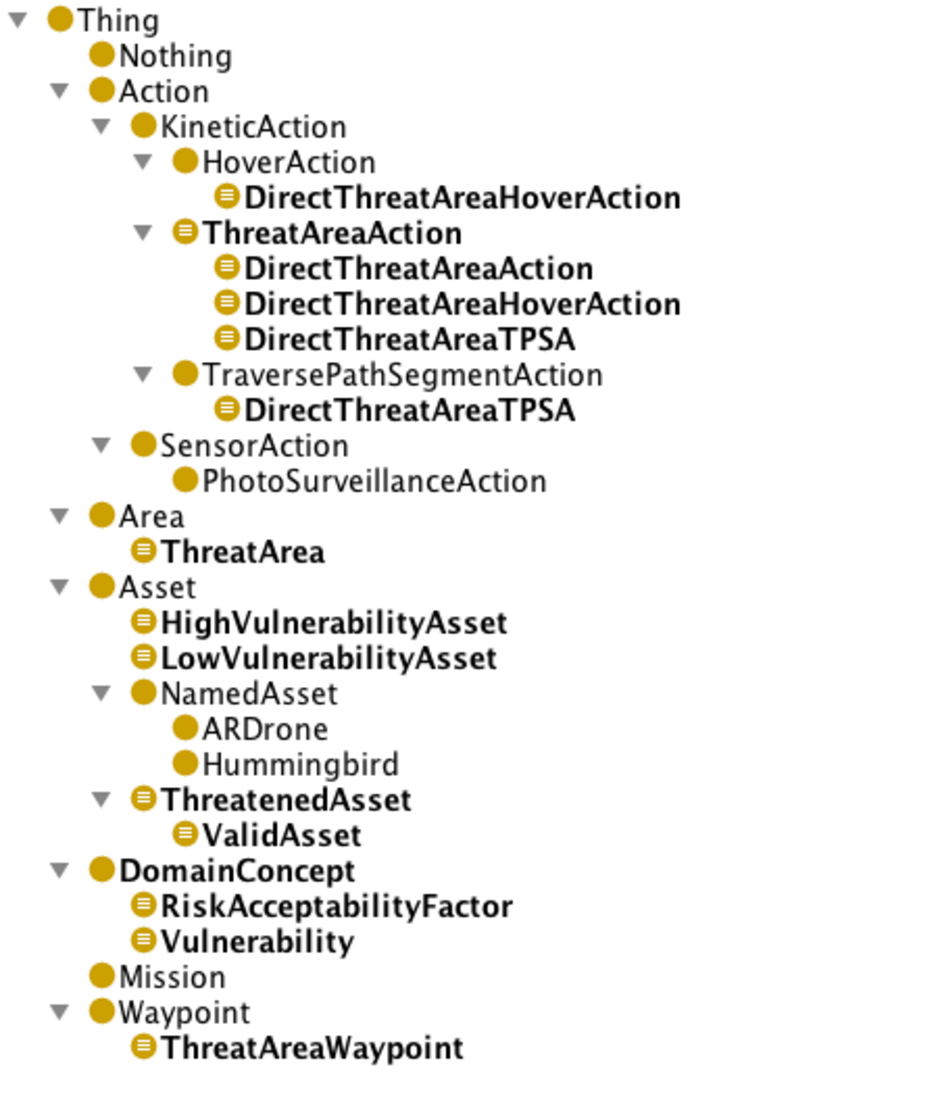
\includegraphics[scale=0.63]{img/tactical-cemo.pdf}
\caption[Tactical-CEMO's class hierarchy]{Tactical-CEMO's multiple inheritance class hierarchy as presented by the Prot\'eg\'e ontology editor.}
\label{fig:tactical_CEMO}
\end{figure}

We define class \texttt{ThreatArea} in Tactical-CEMO and specify that any waypoint related to a threat area be inferred, by Pellet or other semantic reasoners, a member of class \texttt{ThreatAreaWaypoint}. (The geographic information that relates waypoints to threat areas is determined by the CVC during preprocessing, as described in Chapter~\ref{chap:Method_Overview}.) To enable the inference of class membership, class \texttt{ThreatAreaWaypoint} must be \emph{defined} by domain experts using \emph{necessary and sufficient} conditions~\cite{Horridge_2011}. We contrast necessary and sufficient conditions with \emph{necessary} conditions, which describe all classes encoded in CEMO (as described in Section~\ref{sec:Building_an_OWL_Ontology}). These classes are known as \emph{primitive}, and cannot be used to infer class membership. For example, because class \texttt{Asset} is described using only necessary conditions, an individual that is a member of class \texttt{Asset} must satisfy those conditions. However, class membership cannot be inferred for any (random) individual that satisfies the conditions describing class \texttt{Asset}. Figure~\ref{fig:necessary_conditions} illustrates the type of reasoning supported by necessary conditions.

\begin{figure}[ht]
\centering
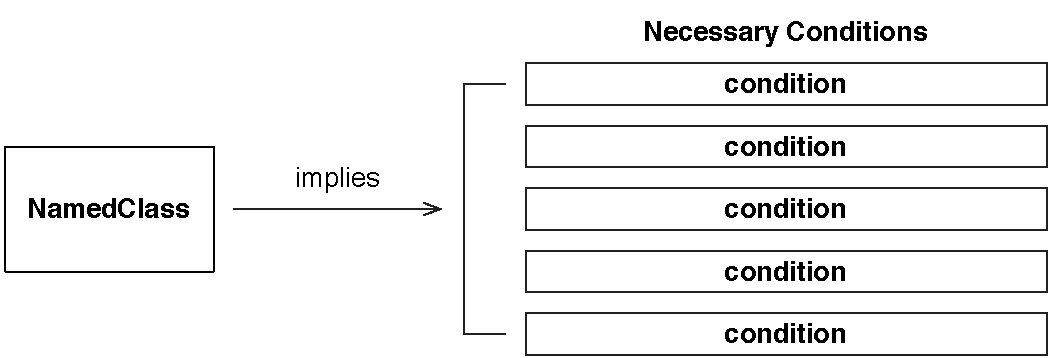
\includegraphics[scale=0.58]{img/necessary-conditions.pdf}
\caption[Primitive classes]{Necessary conditions, which describe primitive classes, cannot be used to infer class membership~\cite{Horridge_2011}. Contrast with Figure~\ref{fig:necessary_and_sufficient_conditions}, which illustrates inference underpinned by necessary and sufficient conditions.}
\label{fig:necessary_conditions}
\end{figure}

Unlike primitive classes, a \emph{defined class}, which is a class comprising necessary and sufficient conditions, can be used to infer class membership. For example, because class \texttt{ThreatAreaWaypoint} is defined using necessary and sufficient conditions, class membership can be inferred for any (random) individual that satisfies those conditions. As with primitive classes, the conditions comprised by class \texttt{ThreatAreaWaypoint} must be satisfied by its members. In other words, class \texttt{ThreatAreaWaypoint} is defined using conditions that are necessary for, and sufficient to infer, class membership. Figure~\ref{fig:necessary_and_sufficient_conditions} illustrates the type of reasoning supported by necessary and sufficient conditions. The OWL code in Listing~\ref{lst:OWL_class_ThreatAreaWaypoint} formally defines class \texttt{ThreatAreaWaypoint}, with the keyword \texttt{EquivalentTo} establishing necessary and sufficient conditions for that class.

\begin{figure}[ht]
\centering
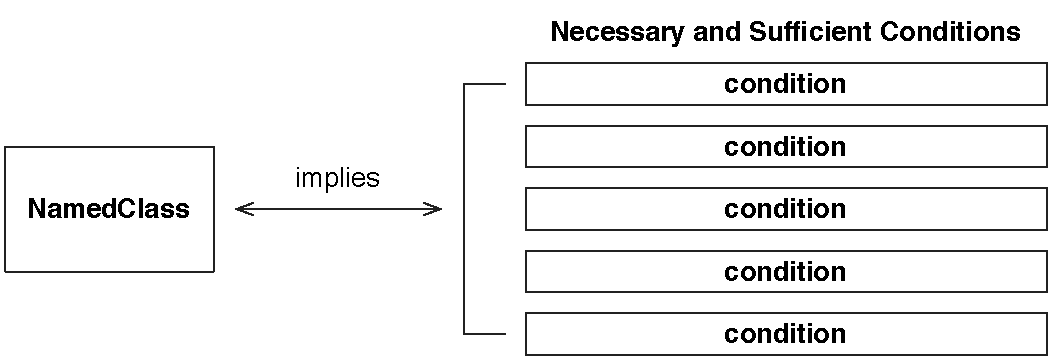
\includegraphics[scale=0.58]{img/necessary-and-sufficient-conditions.pdf}
\caption[Defined classes]{Necessary and sufficient conditions, which are comprised by defined classes, can be used to infer class membership~\cite{Horridge_2011}. Contrast with Figure~\ref{fig:necessary_conditions}, which illustrates inference underpinned by necessary conditions.}
\label{fig:necessary_and_sufficient_conditions}
\end{figure}

\begin{lstlisting}[caption={OWL code for class \texttt{ThreatAreaWaypoint}},label=lst:OWL_class_ThreatAreaWaypoint]
Class: ThreatAreaWaypoint
  EquivalentTo: Waypoint
    and (isWaypointOf some ThreatArea)
\end{lstlisting}

Since members of class \texttt{Waypoint} are associated with \texttt{HoverAction} and \texttt{Traverse\-PathSegmentAction} individuals (see Section~\ref{sec:Building_an_OWL_Ontology}), we specify that any kinetic action related to a threat area waypoint be inferred a member of class \texttt{ThreatAreaAction}. We assert the qualitative difference between \emph{threat area actions} that initiate or prolong an incursion and threat area actions that terminate an incursion, and specify that the former be inferred members of class \texttt{DirectThreatAreaAction}. We further assert the qualitative difference between \emph{direct threat area actions} (DTAAs) that execute exclusively, thereby endangering an asset seemingly without purpose, and those DTAAs that execute concurrently with one or more sensor actions. Given these assertions, we specify that assets with at least one assigned DTAA be inferred members of class \texttt{ThreatenedAsset}. We also specify that a threatened asset with assigned DTAAs be inferred a member of class \texttt{ValidAsset}, if at least one of those DTAAs executes concurrently with at least one sensor action assigned to the same asset. The OWL code in Listing~\ref{lst:OWL_class_ValidAsset} formally defines class \texttt{ValidAsset}.

\begin{lstlisting}[caption={OWL code for class \texttt{ValidAsset}},label=lst:OWL_class_ValidAsset]
Class: ValidAsset
  EquivalentTo: ThreatenedAsset
    and (hasAction some
      (SensorAction
        and (hasSibling some DirectThreatAreaAction)))
\end{lstlisting}

The preceding code contains a nested class expression that is disambiguated with parentheses. This class expression can be understood as follows: A member of class \texttt{ValidAsset} is equivalent to a threatened asset associated, via the object property \texttt{hasAction}, to a member of class \texttt{SensorAction} that is in turn associated, via the object property \texttt{hasSibling}, to a member of class \texttt{DirectThreatAreaAction}. The OWL code in Listing~\ref{lst:OWL_object_property_hasSibling} formally defines \texttt{hasSibling}.

\begin{figure}[ht]
\begin{lstlisting}[caption={OWL code for the object property \texttt{hasSibling}},label=lst:OWL_object_property_hasSibling]
ObjectProperty: hasSibling
  Characteristics: Asymmetric,
    Irreflexive
  Domain: SensorAction
  Range: KineticAction
\end{lstlisting}
\end{figure}

Lines~2 and~3 in Listing~\ref{lst:OWL_object_property_hasSibling} qualify the object property \texttt{hasSibling} with the asymmetric and irreflexive property characteristics, respectively (the transitive property characteristic was introduced in Section~\ref{sec:Building_an_OWL_Ontology}). Because \texttt{hasSibling} is asymmetric\footnote{While potentially counterintuitive, an asymmetric sibling relationship is nevertheless consistent in the context of our domain model.}, if an action~\emph{a} is related via \texttt{hasSibling} to an action~\emph{b}, then~\emph{b} cannot be related to~\emph{a} via the same property. Because \texttt{hasSibling} is irreflexive, if an action~\emph{a} is related via \texttt{hasSibling} to an action~\emph{b}, then~\emph{a} and~\emph{b} cannot be the same action. Figure~\ref{fig:asymmetric_and_irreflexive_properties} illustrates the asymmetric and irreflexive property characteristics that qualify \texttt{hasSibling}.

\begin{figure}[ht]
\centering
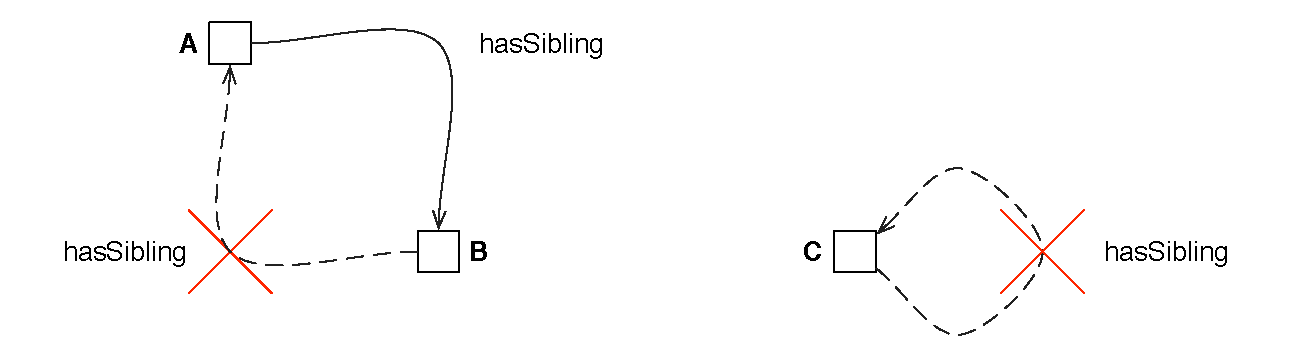
\includegraphics[scale=0.58]{img/asymmetric-irreflexive-properties.pdf}
\caption[Asymmetric and irreflexive properties]{An example of the asymmetric (left) and irreflexive (right) property characteristics that qualify the object property \texttt{hasSibling}. The dashed lines represent inferred relationships.}
\label{fig:asymmetric_and_irreflexive_properties}
\end{figure}

Classes \texttt{ThreatenedAsset} and \texttt{ValidAsset} provide an initial mission verification mechanism in the context of our method. Specifically, a mission specification is inconsistent if it contains threatened assets that are not also \emph{valid assets}. Once the validity of threatened assets has been inferred, the CVC synthesizes DTMC models that enable PRISM to compute the probability of survival for those assets. Accordingly, synthesized models encompass probabilities describing the \emph{vulnerability} of real-world assets. The USDOD defines vulnerability as ``the characteristic of a system that causes it to suffer a definite degradation \ldots\ [resulting from exposure] to a defined level of effects in a man-made hostile environment.''~\cite{DoD_2001} Vulnerability probabilities are derived from classes \texttt{HighVulnerabilityAsset} and \texttt{LowVulnerabilityAsset}, which extend class \texttt{Asset}. The OWL code in Listing~\ref{lst:OWL_class_HighVulnerabilityAsset} formally defines class \texttt{HighVulnerabilityAsset}.

\begin{figure}[ht]
\begin{lstlisting}[caption={OWL code for class \texttt{HighVulnerabilityAsset}},label=lst:OWL_class_HighVulnerabilityAsset]
Class: HighVulnerabilityAsset
  EquivalentTo: Asset
    and (hasCostValue some xsd:integer[<= 1000])
    and (hasSpeedInKilometersPerHour some xsd:integer[<= 20])
  SubClassOf:
    hasRiskAcceptabilityFactor value HighRiskAcceptabilityFactor,
    hasVulnerability value HighVulnerability
  DisjointWith: LowVulnerabilityAsset
\end{lstlisting}
\end{figure}

Similar to class \texttt{Hummingbird}, the ranges of the datatype properties that parameterize members of class \texttt{HighVulnerabilityAsset}, including \texttt{hasCostValue} and \texttt{hasSpeedIn\-KilometersPerHour} (lines~3 and~4, respectively, in Listing~\ref{lst:OWL_class_HighVulnerabilityAsset}), restrict possible datatype values. The datatype property \texttt{hasEnduranceInSeconds}, which is inherited from class \texttt{Asset} (line~2), is not calibrated in a similar manner. The decision to calibrate two of the three inherited datatype properties implies that the calibrated properties are more likely to impact asset vulnerability. We note that, unlike class \texttt{Hummingbird}, the datatype properties in Listing~\ref{lst:OWL_class_HighVulnerabilityAsset} establish necessary and sufficient conditions (lines~1--4), and thereby support the inference of membership for class \texttt{HighVulnerabilityAsset}.

Lines~6 and~7 in Listing~\ref{lst:OWL_class_HighVulnerabilityAsset} use the keyword \texttt{value} to declare \emph{hasValue} restrictions, which describe classes of individuals that must participate in at least one relationship, along a specified property, with a specific individual~\cite{Horridge_2011}. In particular, line~6 specifies that every member of class \texttt{HighVulnerabilityAsset} must be associated with the individual \texttt{HighRiskAcceptabilityFactor} via the object property \texttt{hasRiskAcceptability\-Factor} (the concept of \emph{risk acceptability} will be elaborated in Section~\ref{sec:Modeling_Risk_Acceptability}). Line~7 specifies that every member of class \texttt{HighVulnerabilityAsset} must be associated with the individual \texttt{HighVulnerability} via the object property \texttt{hasVulnerability}. The individuals \texttt{HighRiskAcceptabilityFactor} and \texttt{HighVulnerability} belong, respectively, to the \emph{enumerated classes} \texttt{RiskAcceptabilityFactor} and \texttt{Vulnerability}, which extend the generic class \texttt{DomainConcept}. An enumerated class is defined by listing precisely the individuals that are members of that class. The OWL code in Listing~\ref{lst:OWL_class_Vulnerability} formally defines class \texttt{Vulnerability}.

\begin{lstlisting}[caption={OWL code for class \texttt{Vulnerability}},label=lst:OWL_class_Vulnerability]
Class: Vulnerability
  EquivalentTo: DomainConcept
    and ({HighVulnerability, LowVulnerability})
  DisjointWith: RiskAcceptabilityFactor
\end{lstlisting}

Line~3 in Listing~\ref{lst:OWL_class_Vulnerability} specifies two individuals---\texttt{HighVulnerability} and \texttt{LowVul\-nerability}---that constitute class \texttt{Vulnerability}. The OWL code in Listing~\ref{lst:OWL_individual_HighVulnerability} formally defines the individual \texttt{HighVulnerability}, which is associated with a datatype property describing a double-precision number (line~3). The value of this number is used by the CVC to calculate probabilities that are ultimately integrated into DTMC models representing high vulnerability assets. These modules enable PRISM to compute the probability of survival for high vulnerability assets during threat area incursions. The synthesis process will be elaborated in Section~\ref{sec:Behavioral_Modeling}.

\begin{lstlisting}[caption={OWL code for the individual \texttt{HighVulnerability}},label=lst:OWL_individual_HighVulnerability]
Individual: HighVulnerability
  Types: Vulnerability
  Facts: hasDoubleValue 0.1
\end{lstlisting}

The double-precision number encapsulated by the individual \texttt{HighVulnerability} is the raison d'\^{e}tre for that individual's existence in our ontology. In other words, because datatype properties link classes to data ranges (for example, class \texttt{Hummingbird}) and individuals to data values, we were compelled to create classes of \emph{individuals} that could encapsulate risk acceptability and asset vulnerability \emph{values}. And because the number of individuals per class was finite, enumeration enabled us to explicitly declare the completeness of those classes, and thereby create a finite set of risk acceptability and asset vulnerability grades.

The preceding discussion regarding class \texttt{HighVulnerabilityAsset} applies equally to class \texttt{LowVulnerabilityAsset}, which is formally defined in Listing~\ref{lst:OWL_class_LowVulnerabilityAsset}. Datatype and object property ranges differentiate the two classes.

\begin{lstlisting}[caption={OWL code for class \texttt{LowVulnerabilityAsset}},label=lst:OWL_class_LowVulnerabilityAsset]
Class: LowVulnerabilityAsset
  EquivalentTo: Asset
    and (hasCostValue some xsd:integer[>= 3000])
    and (hasSpeedInKilometersPerHour some xsd:integer[<= 60])
  SubClassOf:
    hasRiskAcceptabilityFactor value LowRiskAcceptabilityFactor
    hasVulnerability value LowVulnerability,
  DisjointWith: HighVulnerabilityAsset
\end{lstlisting}

\subsection{Modeling Traffic Surveillance Missions}
\label{sec:Modeling_Traffic_Surveillance_Missions}

Having investigated tactical missions comprising threat area incursions, we considered a second case study involving traffic surveillance missions. In this scenario, which is conceptually similar to work presented by Heintz et al.~\cite{Heintz_2007}, deployed UAVs are required to monitor freeway traffic and notify subscribers if traffic speeds exceed minimum and nominal thresholds. To accommodate traffic surveillance mission requirements, we have developed a \emph{complex traffic surveillance missions ontology} (Traffic-CEMO) that extends CEMO\@.

Figure~\ref{fig:traffic_CEMO} illustrates Traffic-CEMO's class hierarchy. Classes describing traffic sur\-veillance missions are highlighted in bold, and thereby differentiate from classes encoded in CEMO\@. Also highlighted in bold are classes defined in CEMO that have been declared disjoint from classes defined in Traffic-CEMO\@. Used mainly to support automated reasoning, traffic surveillance concepts are generally not available to mission developers via the YAML DSL\@. Concepts available to mission developers will be highlighted in the analysis that follows.

\begin{figure}[ht]
\centering
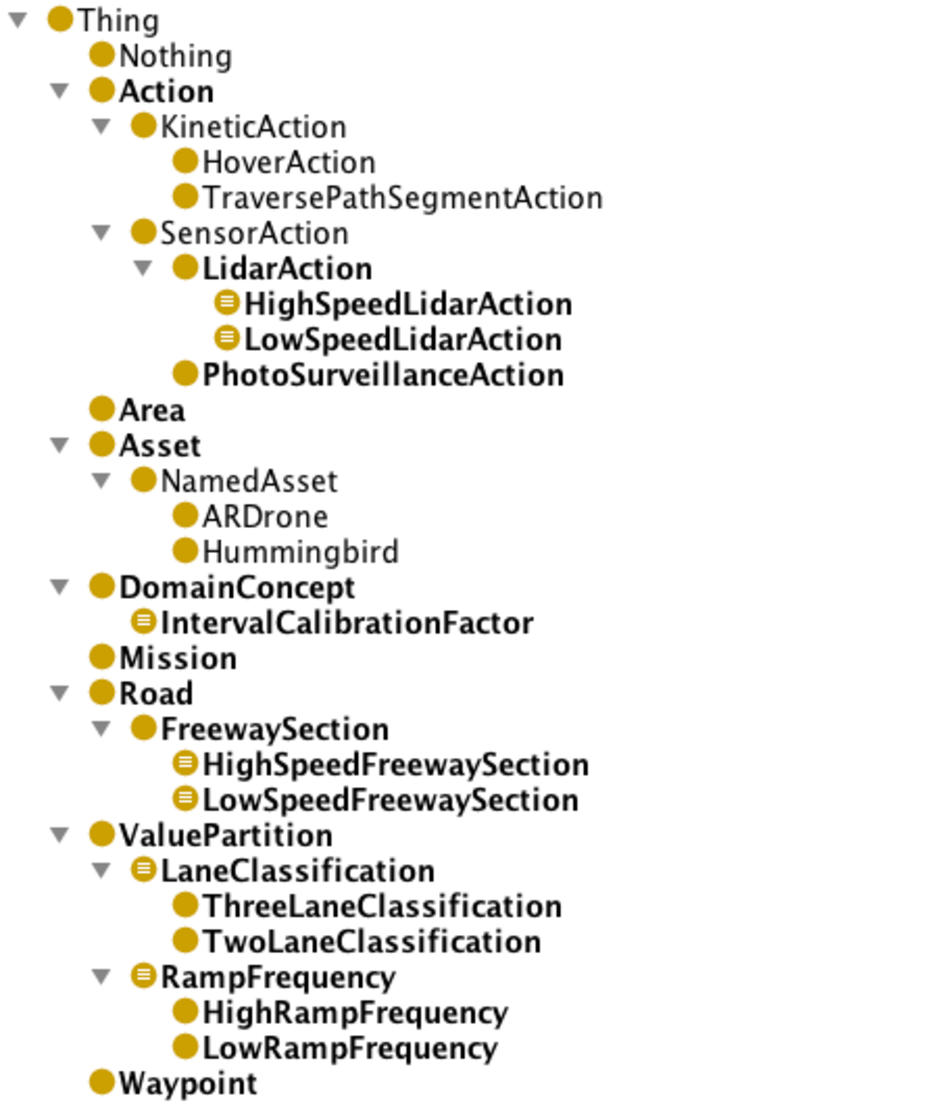
\includegraphics[scale=0.63]{img/traffic-cemo.pdf}
\caption[Traffic-CEMO's class hierarchy]{Traffic-CEMO's class hierarchy as presented by the Prot\'eg\'e ontology editor.}
\label{fig:traffic_CEMO}
\end{figure}

We define class \texttt{FreewaySection} in Traffic-CEMO and specify that two-lane freeway sections with high access ramp frequency be inferred, by Pellet or other semantic reasoners, members of \texttt{FreewaySection} subclass \texttt{LowSpeedFreewaySection}. We also specify that three-lane freeway sections with low access ramp frequency be inferred members of \texttt{FreewaySection} subclass \texttt{HighSpeedFreewaySection}. These inferred relationships formalize the correlation between off-ramp over-saturation and freeway bottlenecks that disrupt traffic discharge rates~\cite{Cassidy_2002}. The OWL code in Listing~\ref{lst:OWL_class_FreewaySection} formally defines class \texttt{FreewaySection}.

\begin{lstlisting}[caption={OWL code for class \texttt{FreewaySection}},label=lst:OWL_class_FreewaySection]
Class: FreewaySection
  SubClassOf: Road,
    approachesMinimumSpeed some xsd:double,
    exceedsMinimumSpeed some xsd:double,
    exceedsNominalSpeed some xsd:double,
    hasLaneClassification some LaneClassification,
    hasRampFrequency some RampFrequency
\end{lstlisting}

Line~3 in Listing~\ref{lst:OWL_class_FreewaySection} associates members of class \texttt{FreewaySection} with the datatype property \texttt{approachesMinimumSpeed}, which describes the potential for minimum traffic speeds to be approached during the operation of freeway sections. The datatype properties \texttt{exceedsMinimumSpeed} (line~4) and \texttt{exceedsNominalSpeed} (line~5) likewise describe the potential for minimum and nominal traffic speeds, respectively, to be exceeded during the operation of freeway sections. Lines~6 and~7 specify that every member of class \texttt{FreewaySection} must be associated, via the object properties \texttt{hasLaneClassification} and \texttt{hasRampFrequency}, with members of classes \texttt{LaneClassification} and \texttt{RampFre\-quency}, respectively. These classes extend class \texttt{ValuePartition}, which represents the \emph{value partition} design pattern~\cite{Horridge_2011}.

We use value partitions to describe the concepts of \emph{lane classification} and on/off \emph{ramp frequency}, and to restrict the range of possible values for those concepts to an exhaustive list of mutually exclusive choices. For example, class \texttt{LaneClassification} restricts the range of the object property \texttt{hasLaneClassification} to classes \texttt{TwoLaneClassifica\-tion} and \texttt{ThreeLaneClassification}. The OWL code in Listing~\ref{lst:OWL_class_LaneClassification} formally defines class \texttt{LaneClassification}.

\begin{lstlisting}[caption={OWL code for class \texttt{LaneClassification}},label=lst:OWL_class_LaneClassification]
Class: LaneClassification
  EquivalentTo: TwoLaneClassification
    or ThreeLaneClassification
  SubClassOf: ValuePartition
  DisjointWith: RampFrequency
\end{lstlisting}

Lines~1--3 in Listing~\ref{lst:OWL_class_LaneClassification} specify a \emph{covering axiom}. This type of axiom comprises a set of classes that \emph{cover} a common superclass by virtue of their union; for example, \texttt{LaneClassification} subtypes \texttt{TwoLaneClassification} and \texttt{ThreeLaneClassifi\-cation} form a union (lines~2 and~3) that covers their common superclass. We note that the union of classes \texttt{TwoLaneClassification} and \texttt{ThreeLaneClassification} establishes necessary and sufficient conditions for class \texttt{LaneClassification} (necessary and sufficient conditions were described in Section~\ref{sec:Modeling_Tactical_Missions}). The OWL code in Listing~\ref{lst:OWL_class_TwoLaneClassification} formally defines class \texttt{TwoLaneClassification}.

\begin{lstlisting}[caption={OWL code for class \texttt{TwoLaneClassification}},label=lst:OWL_class_TwoLaneClassification]
Class: TwoLaneClassification
  SubClassOf: LaneClassification
  DisjointWith: ThreeLaneClassification
\end{lstlisting}

Line~3 in Listing~\ref{lst:OWL_class_TwoLaneClassification} specifies that classes \texttt{TwoLaneClassification} and \texttt{ThreeLane\-Classification} constitute disjoint sets of individuals. Because class \texttt{LaneClassifica\-tion} is \emph{covered} by the union of its two subclasses, and because those subclasses are disjoint, a member of class \texttt{LaneClassification} must also be a member of either \texttt{TwoLaneClassification} or \texttt{ThreeLaneClassification}. As with enumeration, which was described in Section~\ref{sec:Modeling_Tactical_Missions}, value partitions enabled us to create a finite set of possible values (in this case, lane classification and ramp frequency grades). The value partitions that describe lane classification and ramp frequency are used to parameterize \texttt{FreewaySection} subtypes including classes \texttt{LowSpeedFreewaySection} and \texttt{HighSpeed\-FreewaySection}. The OWL code in Listing~\ref{lst:OWL_class_HighSpeedFreewaySection} formally defines the latter class.

\begin{figure}[ht]
\begin{lstlisting}[caption={OWL code for class \texttt{HighSpeedFreewaySection}},label=lst:OWL_class_HighSpeedFreewaySection]
Class: HighSpeedFreewaySection
  EquivalentTo: FreewaySection
    and (hasLaneClassification some ThreeLaneClassification)
    and (hasRampFrequency some LowRampFrequency)
  SubClassOf: approachesMinimumSpeed some xsd:double[>= 0.2],
    exceedsMinimumSpeed some xsd:double[>= 0.9],
    exceedsNominalSpeed some xsd:double[>= 0.5]
  DisjointWith: LowSpeedFreewaySection
\end{lstlisting}
\end{figure}

Lines~1--4 in Listing~\ref{lst:OWL_class_HighSpeedFreewaySection} use value partitions to establish necessary and sufficient conditions, and thereby support the inference of membership for class \texttt{HighSpeedFreeway\-Section}. Unlike class \texttt{FreewaySection}, the ranges of the datatype properties that parameterize members of class \texttt{HighSpeedFreewaySection} (lines~5--7) restrict possible data values. These data values specify probabilities for traffic speed fluctuations during the operation of high-speed freeway sections. Traffic speed fluctuations affect the optimal surveillance of freeway traffic by airborne \emph{light detection and ranging} (LIDAR) systems.

LIDAR is an optical remote sensing technology that can observe targets from a distance of 15 kilometers (in air) with sub-millimeter resolution~\cite{Piracha_2010}. The integration of LIDAR systems into rotary wing UAV platforms could enable, for example, a single hovering UAV with a five kilometer altitude ceiling to monitor traffic over an area spanning approximately 630 square kilometers. In the context of an urban environment, LIDAR-equipped UAVs offer a flexible and optimizable alternative to land-based cameras for the simultaneous surveillance of multiple freeway sections. The OWL code in Listing~\ref{lst:OWL_class_LidarAction} models the concept of LIDAR systems by formally defining class \texttt{LidarAction} as a sensor action subtype.

\begin{lstlisting}[caption={OWL code for class \texttt{LidarAction}},label=lst:OWL_class_LidarAction]
Class: LidarAction
  SubClassOf: SensorAction,
    hasIntervalInSeconds some xsd:integer,
    hasIntervalCalibrationFactor some IntervalCalibrationFactor,
    isConcurrentWith some HoverAction
  DisjointWith: PhotoSurveillanceAction
\end{lstlisting}

The object property \texttt{hasIntervalCalibrationFactor} (line~4 in Listing~\ref{lst:OWL_class_LidarAction}) links LIDAR actions with the individuals \texttt{HighIntervalCalibrationFactor} and \texttt{LowInter\-valCalibrationFactor}, which constitute the enumerated class \texttt{IntervalCalibration\-Factor}. Members of class \texttt{IntervalCalibrationFactor} are associated with a datatype property describing an integer. The value of this integer, which is ultimately integrated into DTMC models that simulate LIDAR actions, calibrates intervals between LIDAR readings. LIDAR intervals are specified by mission developers with a construct from our DSL; the interval type that verifies mission plans is specified by the datatype property \texttt{hasIntervalInSeconds} (line~5). Every member of class \texttt{LidarAction} is also associated, via the object property \texttt{isConcurrentWith} (line~3), with a \texttt{HoverAction} individual. This relationship is specified by mission developers via the YAML DSL\@.

Class \texttt{LidarAction} is extended by class \texttt{HighSpeedLidarAction}, which is formally defined by the OWL code in Listing~\ref{lst:OWL_class_HighSpeedLidarAction}. \texttt{LidarAction} subtype individuals are associated with members of class \texttt{HighSpeedFreewaySection} via the object property \texttt{monitors} (line~3). Given the necessary and sufficient conditions established in Listing~\ref{lst:OWL_class_HighSpeedLidarAction} (lines~1--3), LIDAR actions that monitor \emph{high-speed freeway sections} are inferred members of class \texttt{HighSpeedLidarAction}. Thus \texttt{FreewaySection} subtypes support inferences that determine the classification of \texttt{LidarAction} individuals. The object property \texttt{monitors}, which encompasses the concurrency relationship specified by mission developers, will be elaborated in Section~\ref{sec:Rule_Based_Modeling}.

\begin{lstlisting}[caption={OWL code for class \texttt{HighSpeedLidarAction}},label=lst:OWL_class_HighSpeedLidarAction]
Class: HighSpeedLidarAction
  EquivalentTo: LidarAction
    and (monitors some HighSpeedFreewaySection)
  SubClassOf: hasIntervalCalibrationFactor value HighIntervalCalibrationFactor
  DisjointWith: LowSpeedLidarAction
\end{lstlisting}

Line~4 in Listing~\ref{lst:OWL_class_HighSpeedLidarAction} links \texttt{HighSpeedLidarAction} individuals with a \emph{high interval calibration factor}, which is integrated into DTMC models representing \emph{high-speed LIDAR actions}. Thus \texttt{LidarAction} classifications support the synthesis of DTMC artifacts that model the behavior of LIDAR action individuals. The discussion regarding class \texttt{HighSpeedLidarAction} applies equally to class \texttt{LowSpeedLidarAction}, which is formally defined in Listing~\ref{lst:OWL_class_LowSpeedLidarAction}. Object property ranges differentiate the two classes.

\begin{lstlisting}[caption={OWL code for class \texttt{LowSpeedLidarAction}},label=lst:OWL_class_LowSpeedLidarAction]
Class: LowSpeedLidarAction
  EquivalentTo: LidarAction
    and (monitors some LowSpeedFreewaySection)
  SubClassOf: hasIntervalCalibrationFactor value LowIntervalCalibrationFactor
  DisjointWith: HighSpeedLidarAction
\end{lstlisting}

Appendix~\ref{chap:Ontology} presents CEMO, Tactical-CEMO and Traffic-CEMO in their entirety.

\subsection{An Overview}

Section~\ref{sec:Semantic_Modeling} exploits OWL to formalize a subset of the UAV domain. With respect to the OWL constructs presented in Section~\ref{sec:OWL_SWRL_and_Prolog}: Listing~\ref{lst:OWL_class_ThreatAreaWaypoint} uses the equivalence predicate \texttt{EquivalentTo} to establish necessary and sufficient conditions for class \texttt{ThreatArea\-Waypoint}. Listing~\ref{lst:OWL_class_Hummingbird} uses the primitive \texttt{DisjointWith} to specify that classes \texttt{ARDrone} and \texttt{Hummingbird} constitute disjoint sets. And Listing~\ref{lst:OWL_class_Vulnerability} uses enumeration to describe class \texttt{Vulnerability}. These and other OWL-based modeling methods described throughout Section~\ref{sec:Semantic_Modeling} support the expressive representation of knowledge by domain experts.

OWL also supports the efficient reasoning afforded by Pellet. Two strands of reasoning are particularly compelling because they span multiple classes and relationships. Tactical-CEMO comprises the inferred concepts \texttt{DirectThreatAreaAction} and \texttt{ValidAsset}; these concepts support the synthesis or PRISM code from templates, which will be presented in Section~\ref{sec:Modeling_Survivability} and Section~\ref{sec:Modeling_Risk_Acceptability}. Traffic-CEMO also comprises inferred concepts including \texttt{HighSpeedFreewaySection} and \texttt{HighSpeedLidarAction}, which support the synthesis of PRISM code from templates presented in Section~\ref{sec:Modeling_Traffic_Surveillance}. The OWL-based inferences described throughout Section~\ref{sec:Semantic_Modeling} enable the CVC to generate low-level system models and their desired behavioral properties from high-level system specifications encoded by model builders.

\section{Rule-Based Modeling}
\label{sec:Rule_Based_Modeling}

OWL is a powerful knowledge representation formalism, but expressive and reasoning limitations constrain its utility; for example, OWL cannot model \emph{cross-cutting actions}. We consider an action \emph{a} to be cross-cutting if~\emph{a} is a precondition to an action~\emph{b}, and~\emph{b} is assigned to an asset that is different from the asset to which~\emph{a} is assigned. By this definition, action \texttt{TPSA3} in Mission~A is a \emph{cross-cutting kinetic action}. The OWL code in Listing~\ref{lst:OWL_class_CrossCuttingKineticAction} presents an incomplete definition of class \texttt{CrossCuttingKineticAction}.

\begin{lstlisting}[caption={OWL code for class \texttt{CrossCuttingKineticAction}},label=lst:OWL_class_CrossCuttingKineticAction]
Class: CrossCuttingKineticAction
  EquivalentTo: KineticAction
    and (isActionOf some Asset)
    and (hasPrecondition some
      (Action
        and (isActionOf some Asset)))
\end{lstlisting}

The definition in Listing~\ref{lst:OWL_class_CrossCuttingKineticAction} is lacking because the asset in line~3 cannot be differentiated from the asset in line~6. The SWRL code in Listing~\ref{lst:SWRL_rule_CrossCuttingKineticAction} uses the built-in OWL property \texttt{differentFrom} to appropriately define class \texttt{CrossCuttingKineticAction} (question mark prefixes denote variables). The OWL code in line~1 provides a rudimentary definition for the \texttt{CrossCuttingKineticAction} concept, which is augmented by the rule in lines 3--12.

\begin{figure}[ht]
\begin{lstlisting}[caption={OWL+SWRL code for rule \texttt{CrossCuttingKineticAction}},label=lst:SWRL_rule_CrossCuttingKineticAction]
Class: CrossCuttingKineticAction

Rule:
    KineticAction(?a),
    KineticAction(?b),
    Asset(?x),
    Asset(?y),
    hasAction(?x, ?a),
    hasAction(?y, ?b),
    hasPrecondition(?b, ?a),
    DifferentFrom(?x, ?y)
  -> CrossCuttingKineticAction(?a)
\end{lstlisting}
\end{figure}

The SWRL rule in Listing~\ref{lst:SWRL_rule_CrossCuttingKineticAction} augments the definition of an OWL class. Listing~\ref{lst:SWRL_rule_monitors} uses a SWRL rule to augment the OWL object property \texttt{monitors}, which supports inferences described in Section~\ref{sec:Modeling_Traffic_Surveillance_Missions}. Lines~1--5 formally define \texttt{monitors} as an asymmetric and irreflexive object property with domain and range the classes \texttt{LidarAction} and \texttt{FreewaySection}, respectively (similar definitions have been introduced throughout this chapter). Line~14 specifies that a LIDAR action~\emph{?l} (defined in line~10) monitors a freeway section~\emph{?f} (defined in line~8) if the hover action~\emph{?h} (defined in line~9) that executes concurrently with~\emph{?l} (as specified in line~13) is associated with a waypoint~\emph{?w} (as specified in line~11) that also delineates~\emph{?f} (as specified in line~12).

\begin{lstlisting}[caption={OWL+SWRL code for rule \texttt{monitors}},label=lst:SWRL_rule_monitors]
ObjectProperty: monitors
  Characteristics: Asymmetric,
    Irreflexive
  Domain: LidarAction
  Range: FreewaySection

Rule:
    FreewaySection(?f),
    HoverAction(?h),
    LidarAction(?l),
    hasWaypoint(?f, ?w),
    hasWaypoint(?h, ?w),
    isConcurrentWith(?l, ?h)
  -> monitors(?l, ?f)
\end{lstlisting}

SWRL rules extend the expressive power of OWL; but like OWL, SWRL cannot reason effectively with negation. Rules that must reason with negation are therefore encoded in Prolog. Domain knowledge is negated during the ontology development process if Pellet reasoning with respect to that knowledge is deemed unattainable. The Prolog code in Listing~\ref{lst:Prolog_rule_terminal} formally defines rule \texttt{terminal}, which comprises three negated atoms (an atom is the basic building block of a Prolog rule). Rule \texttt{terminal} encapsulates both explicit and inferred ontological knowledge; explicit knowledge is encoded with the atom \texttt{has\_action} (line~2), while the three negated atoms (lines~3--5) encode knowledge inferred by Pellet.

\begin{lstlisting}[caption={Prolog code for rule \texttt{terminal}},label=lst:Prolog_rule_terminal]
terminal(X) :-
    has_action(A, X),
    not(is_precondition_to(X, _)),
    not(single_action_asset(A)),
    not(zero_action_asset(A)).
\end{lstlisting}

The transition of inferred knowledge from OWL to Prolog can be illustrated with the atom \texttt{is\_precondition\_to} (line~3 in Listing~\ref{lst:Prolog_rule_terminal}). The OWL code in Listing~\ref{lst:OWL_object_property_isPreconditionTo} formally defines the object property \texttt{isPreconditionTo}, a relationship that inverts the object property \texttt{hasPrecondition}. This inversion constitutes a Pellet inference (as described in Section~\ref{sec:Semantic_Modeling}).

\begin{lstlisting}[caption={OWL code for the object property \texttt{isPreconditionTo}},label=lst:OWL_object_property_isPreconditionTo]
ObjectProperty: isPreconditionTo
  InverseOf: hasPrecondition
  (*\ldots*)
\end{lstlisting}

Mission~A comprises several instances of the DSL construct \texttt{preconditions} (lines~10, 18 and~22 in Listing~\ref{lst:Mission_A}). The CVC transforms knowledge contained in this construct into knowledge encoded as property \texttt{hasPrecondition}. Knowledge inferred by Pellet with respect to \texttt{hasPrecondition}, via the inverted property \texttt{isPreconditionTo}, is transformed by the CVC into knowledge encoded with the atom \texttt{is\_precondition\_to}, which in turn supports SWI-Prolog inferences.

Appendix~\ref{chap:Ontology} and Appendix~\ref{chap:Prolog_Knowledge_Base} present, respectively, the SWRL and Prolog rule-bases in their entirety.

\subsection{An Overview}

Section~\ref{sec:Rule_Based_Modeling} exploits SWRL to overcome OWL limitations and encode complex relational structures. SWRL rules in Listing~\ref{lst:SWRL_rule_CrossCuttingKineticAction} and Listing~\ref{lst:SWRL_rule_monitors} augment class \texttt{CrossCutting\-KineticAction} and the object property \texttt{monitors}, respectively. The inferred concept \texttt{CrossCuttingKineticAction} supports PRISM code synthesis via a process that will be described in Chapter~\ref{chap:Cascading_Verification}. In conjunction with several inferred concepts, including \texttt{HighSpeedFreewaySection} and \texttt{HighSpeedLidarAction}, the object property \texttt{monitors} supports the synthesis of PRISM code from templates, which will be presented in Section~\ref{sec:Modeling_Traffic_Surveillance}.

Prolog is used to overcome OWL+SWRL limitations and encode knowledge that can support effective reasoning with negation. Listing~\ref{lst:Prolog_rule_terminal} and Listing~\ref{lst:OWL_object_property_isPreconditionTo} illustrate composite FOL reasoning, which is reasoning supported by multiple and integrated FOL-based systems, with the transition of inferred knowledge from OWL to Prolog. The process that leverages composite reasoning to synthesize PRISM code will be described in Chapter~\ref{chap:Cascading_Verification}.

\section{Behavioral Modeling}
\label{sec:Behavioral_Modeling}

OWL+SWRL and Prolog are appropriate formalisms for encoding semantic and rule-based knowledge. Likewise, the state-based PRISM modeling language is an appropriate formalism for encoding behavioral knowledge as DTMC models. The PRISM language can thus form the basis for reusable DTMC templates.

The code in Listing~\ref{lst:DTMC_asset_module_template} uses string interpolation, which is denoted by the code snippet \texttt{\#\{ \ldots\ \}}, to encapsulate parameters in the context of a DTMC template for asset modules. The \emph{module} is a fundamental PRISM language construct. The asset module template encodes knowledge that describes the behavior of the \texttt{Asset} concept encoded in CEMO\@.

\begin{lstlisting}[caption={DTMC template for asset modules},label=lst:DTMC_asset_module_template]
module #{asset.class}#{asset.id}
  e#{asset.id} : [0..#{asset.endurance}] init #{asset.endurance};
  (*\colorbox{yellow!25}{FOR action IN asset.kinetic\_actions DO}*)
  [#{(*{\color{blue}action.type}*)}] e#{asset.id}>0 & d#{action.id}>0
      -> (e#{asset.id}'=e#{asset.id}-1);
  (*\colorbox{yellow!25}{END}*)
  [#{(*{\color{blue}asset.last\_action.type}*)}] e#{asset.id}=0 | d#{(*{\color{purple}asset.last\_action.id}*)}=0
      -> true;
endmodule
\end{lstlisting}

A module definition contains \emph{variables} and \emph{commands}. Asset module states are stored in variable \texttt{e\#\{asset.id\}} (lines~2, 4, 5 and~7 in Listing~\ref{lst:DTMC_asset_module_template}), which represents asset endurance. Line~2 declares \texttt{e\#\{asset.id\}} to be an integer variable with range \texttt{[0..\#\{asset.endurance\}]}. The upper limit for the range is derived from \texttt{asset.en\-durance}, which also initializes \texttt{e\#\{asset.id\}} (as denoted by the keyword \texttt{init}).

Asset behavior is formalized with two or more commands, where each command assumes the form:

\begin{quote}
$[action]\:guard \rightarrow P(update_1) : update_1 + \ldots + P(update_n) : update_n;$
\end{quote}

\noindent A command becomes \emph{enabled} for execution when its \emph{guard} is satisfied by a specific model state; for example, lines~4 and~5 in Listing~\ref{lst:DTMC_asset_module_template} specify a command that becomes enabled when action duration, which is denoted by variable \texttt{d\#\{action.id\}}, \emph{and} asset endurance exceed zero. Commands encompass one or more updates, where each \emph{update} transitions a module, with a given probability, from one state to the next. A probability of one is assumed, and can therefore be omitted, for commands with single updates. Each command may be labeled with an \emph{action}, which forces two or more modules to transition states simultaneously (i.e., to synchronize).

Lines~3 and~6 in Listing~\ref{lst:DTMC_asset_module_template} use meta-code, which is highlighted with yellow background, to define a for loop. The form assumed by each for loop is

\begin{quote}
\begin{lstlisting}[frame=none,numbers=none]
(*\colorbox{yellow!25}{FOR var IN collection DO}*) body (*\colorbox{yellow!25}{END}*)
\end{lstlisting}
\end{quote}

\noindent where \texttt{var} denotes a variable and \texttt{collection} denotes a collection of objects. Each asset module command generated by the for loop in Listing~\ref{lst:DTMC_asset_module_template} represents the execution of a kinetic action. The \texttt{true} keyword in the last command (line~8) denotes the end of execution for a specific module. This type of command prevents deadlocks that are inconsequential to mission correctness from terminating the verification process with an error.

Arguments for the parameters in Listing~\ref{lst:DTMC_asset_module_template} are derived from explicit and inferred domain knowledge. Specifically, arguments for \texttt{asset.class} (line~1) and \texttt{asset.id} (lines~1, 2, 4, 5 and~7) are derived from mission plans; arguments for \texttt{asset.endurance} (line~2) are derived from explicit domain knowledge encoded in CEMO; and arguments for \texttt{action.type} (line~4), \texttt{asset.last\_action.type} (line~7) and \texttt{asset.last\_action.id} (line~7) are derived from knowledge inferred by Pellet and the Prolog compiler (via a process that will be described in Chapter~\ref{chap:Cascading_Verification}). Listing~\ref{lst:DTMC_asset_module_template} uses blue text to highlight parameters that receive as arguments domain-specific knowledge encoded by domain experts and derived from inferences. Purple text highlights parameters that receive as arguments mission-specific knowledge encoded by mission developers and also derived from inferences. This color coding scheme will be used for the remainder of Chapter~\ref{chap:Domain_Modeling}.

Mission properties are encoded in PRISM's property specification language, which subsumes several probabilistic temporal logics including PCTL, CSL and LTL\@. The code in Listing~\ref{lst:PCTL_action_duration_template} formally defines a mission property template. This generic property queries the probability that an action with identifier \texttt{action.id} will deplete its duration---as denoted by the assertion \texttt{d\#\{action.id\}=0}---and thereby complete its execution. An ellipsis indicates the potential for synthesized properties to comprise multiple assertions. Arguments for the parameter \texttt{action.id} are derived from knowledge inferred by Pellet and the Prolog compiler (via a process that will be described in Chapter~\ref{chap:Cascading_Verification}).

\begin{lstlisting}[caption={PCTL template for action duration},label=lst:PCTL_action_duration_template]
P=? [ F d#{(*{\color{purple}action.id}*)}=0 (*\ldots\hspace{1.8mm}*)]
\end{lstlisting}

\subsection{Modeling Survivability}
\label{sec:Modeling_Survivability}

Asset module commands comprise single updates that omit probabilities. The code in Listing~\ref{lst:DTMC_asset_survivability_template} formally defines a template for asset survivability modules, which contain commands with multiple updates. Survivability modules enable PRISM to calculate the probability of survival for \texttt{ValidAsset} individuals with respect to the threat area actions executed by each asset (valid assets were described in Section~\ref{sec:Modeling_Tactical_Missions}). Module states are stored in the boolean variable \texttt{a\#\{asset.id\}d} (defined in line~9 and used in lines~11--14), which represents the destruction of the asset with identifier \texttt{asset.id}. Command updates transition survivability modules from one state to the next. The probability of execution for each update is derived from the parameter \texttt{asset.vulnerability} (lines~12 and~13). Current vulnerability values are arbitrary, and should eventually be calculated from real-world data related to asset capabilities, terrain types and weather conditions.

\begin{figure}[ht]
\begin{lstlisting}[caption={DTMC template for asset survivability},label=lst:DTMC_asset_survivability_template]
(*\colorbox{yellow!25}{FOR action IN asset.threat\_area\_actions DO}*)
const int start#{(*{\color{purple}action.id}*)} = #{(*{\color{purple}action.start}*)};
const int finish#{(*{\color{purple}action.id}*)} = #{(*{\color{purple}action.finish}*)};
formula actn#{(*{\color{purple}action.id}*)}_tai = d#{(*{\color{purple}action.id}*)}>finish#{(*{\color{purple}action.id}*)} &
    d#{(*{\color{purple}action.id}*)}<=start#{(*{\color{purple}action.id}*)};
(*\colorbox{yellow!25}{END}*)

module #{(*{\color{purple}asset.class}*)}#{(*{\color{purple}asset.id}*)}_Survivability
  a#{(*{\color{purple}asset.id}*)}d : bool init false;
  (*\colorbox{yellow!25}{FOR action IN asset.threat\_area\_actions DO}*)
  [#{(*{\color{blue}action.type}*)}] !a#{(*{\color{purple}asset.id}*)}d & actn#{(*{\color{purple}action.id}*)}_tai
      -> #{1-(*{\color{purple}asset.vulnerability}*)}:(a#{(*{\color{purple}asset.id}*)}d'=false) +
         #{(*{\color{purple}asset.vulnerability}*)}:(a#{(*{\color{purple}asset.id}*)}d'=true);
  [#{(*{\color{blue}action.type}*)}] a#{(*{\color{purple}asset.id}*)}d | !actn#{(*{\color{purple}action.id}*)}_tai
      -> true;
  (*\colorbox{yellow!25}{END}*)
endmodule
\end{lstlisting}
\end{figure}

Lines~1 and~6 in Listing~\ref{lst:DTMC_asset_survivability_template} use meta-code to define a for loop that generates one \emph{formula} with identifier \texttt{actn\#\{action.id\}\_tai} (defined in line~4 and used in lines~11 and~14) per each action assigned to the asset in the loop header (the formula is a PRISM language construct used to avoid code duplication). Each formula specifies an overlap between the prosecution of a threat area incursion and the execution of a threat area action with identifier \texttt{action.id} (threat area actions were described in Section~\ref{sec:Modeling_Tactical_Missions}). This overlap is delineated by variables \texttt{start\#\{action.id\}} and \texttt{finish\#\{action.id\}} (defined in lines~2 and~3, respectively), which are assigned geographic information calculated by the CVC during preprocessing (as described in Chapter~\ref{chap:Method_Overview}).

The constructs \texttt{a\#\{asset.id\}d} and \texttt{actn\#\{action.id\}\_tai} combine to form logical expressions, including a logical conjunction and disjunction (lines~11 and~14, respectively), that constitute the guards in the asset survivability module. When these expressions are considered in union, their logical truth values, which are highlighted in Table~\ref{tab:asset_survivability_module_truth_table}, clarify asset behavior and susceptibility during threat area incursions. Specifically, a valid asset exists in one of the following disjoint states:

\begin{itemize}

\item \emph{not} destroyed and prosecuting a threat area incursion, whereby the logical conjunction is true;

\item destroyed, as a consequence of prosecuting a threat area incursion, or \emph{not} prosecuting a threat area incursion, whereby the logical disjunction is true.

\end{itemize}

\begin{table}[ht]
	\arrayrulecolor{Gray}
	\renewcommand*\arraystretch{1.3}
	\begin{tabularx}{\textwidth}{
			>{\centering\arraybackslash}X|
			>{\centering\arraybackslash}X|
			>{\centering\arraybackslash}X|
			>{\centering\arraybackslash}X
		}
		$d$ & $tai$ & $!d \wedge tai$ & $d \vee !tai$\\
		\hline
		true & true & false & \cellcolor{green!65}true\\
		\hline
		true & false & false & \cellcolor{green!65}true\\
		\hline
		false & true & \cellcolor{green!65}true & false\\
		\hline
		false & false & false & \cellcolor{green!65}true\\
	\end{tabularx}
	\caption[Asset survivability truth table]{A truth table for asset survivability guards, with variables \texttt{a\#\{asset.id\}d} and \texttt{actn\#\{action.id\}\_tai} in Listing~\ref{lst:DTMC_asset_survivability_template} represented by variables \emph{d} and \emph{tai}, respectively.}
	\label{tab:asset_survivability_module_truth_table}
\end{table}

Arguments for the parameters in Listing~\ref{lst:DTMC_asset_survivability_template} are derived from explicit and inferred domain knowledge. Specifically, arguments for \texttt{action.id} (lines~4, 5, 11 and~14), \texttt{asset.class} (line~8) and \texttt{asset.id} (lines~8, 9 and~11--14) are derived from mission plans; arguments for \texttt{asset.vulnerability} (lines~12 and~13) are derived from knowledge inferred by Pellet; arguments for \texttt{action.start} (line~2), \texttt{action.finish} (line~3) are derived from geodetic calculations and knowledge inferred by Pellet; and arguments for \texttt{action.type} (lines~11 and~14) are derived from knowledge inferred by Pellet and the Prolog compiler.

The generic property in Listing~\ref{lst:PCTL_asset_survivability_template} queries the probability that an asset with identifier \texttt{asset.id} will not be destroyed during its prosecution of threat area incursions. This mission property makes explicit the intuitive correlation between asset survivability and mission correctness.

\begin{lstlisting}[caption={PCTL template for asset survivability},label=lst:PCTL_asset_survivability_template]
P=? [ F !a#{(*{\color{purple}asset.id}*)}d (*\ldots\hspace{1.8mm}*)]
\end{lstlisting}

\subsection{Modeling Risk Acceptability}
\label{sec:Modeling_Risk_Acceptability}

We assert that, during threat area incursions, mission correctness is contingent on asset survivability \emph{and} risk acceptability. As described in Section~\ref{sec:Modeling_Tactical_Missions}, a threat area action that initiates or prolongs an incursion is inferred a member of class \texttt{DirectThreat\-AreaAction}. This inference triggers the synthesis of PRISM code that calculates a \emph{risk acceptability factor} (RAF) for the threat area incursion comprising the inferred DTAA\@. Each RAF value quantifies the risk for a specific threat area incursion, with RAF values of zero and one indicating high- and low-risk incursions, respectively. A RAF numerator represents the duration of concurrent execution between sensor actions and DTAAs during a threat area incursion; the denominator represents the aggregate duration of DTAA executions during that incursion.

The code in Listing~\ref{lst:DTMC_risk_acceptability_template} formally defines a template that enables PRISM to calculate risk acceptability with respect to the threat area incursions prosecuted by a \texttt{ValidAsset} individual. For a given asset, RAF values quantifying the incursions prosecuted by that asset are aggregated by the formula with identifier \texttt{raf\#\{asset.id\}} (line~39). Numerator and denominator for this formula are derived, respectively, from the constructs \texttt{sad\#\{asset.id\}} and \texttt{tkad\#\{asset.id\}}.

\begin{figure}[!ht]
\begin{lstlisting}[caption={DTMC template for risk acceptability},label=lst:DTMC_risk_acceptability_template]
(*\colorbox{yellow!25}{FOR action IN asset.direct\_threat\_area\_actions DO}*)
const int start#{(*{\color{purple}action.id}*)} = #{(*{\color{purple}action.start}*)};
const int finish#{(*{\color{purple}action.id}*)} = #{(*{\color{purple}action.finish}*)};
formula actn#{(*{\color{purple}action.id}*)}_tai = d#{(*{\color{purple}action.id}*)}>finish#{(*{\color{purple}action.id}*)} &
    d#{(*{\color{purple}action.id}*)}<=start#{(*{\color{purple}action.id}*)};
formula duration#{(*{\color{purple}action.id}*)} = start#{(*{\color{purple}action.id}*)} - finish#{(*{\color{purple}action.id}*)};
(*\colorbox{yellow!25}{END}*)

formula tkad#{(*{\color{purple}asset.id}*)} =
    (*\colorbox{yellow!25}{FOR action IN asset.direct\_threat\_area\_actions DO}*)
    duration#{(*{\color{purple}action.id}*)}
    + (*\colorbox{yellow!25}{IF action != asset.direct\_threat\_area\_actions.last}*)
    (*;*) (*\colorbox{yellow!25}{IF action == asset.direct\_threat\_area\_actions.last}*)
    (*\colorbox{yellow!25}{END}*)

module SensorActionCounter#{(*{\color{purple}asset.id}*)}
  sad#{(*{\color{purple}asset.id}*)} : [0..tkad#{(*{\color{purple}asset.id}*)}] init 0;
  (*\colorbox{yellow!25}{FOR action IN asset.direct\_threat\_area\_actions DO}*)
  [#{(*{\color{blue}action.type}*)}] actn#{(*{\color{purple}action.id}*)}_tai &
      (
          (*\colorbox{yellow!25}{FOR sensor\_action IN asset.sensor\_actions DO}*)
          r#{(*{\color{purple}sensor\_action.id}*)}
          | (*\colorbox{yellow!25}{IF sensor\_action != asset.sensor\_actions.last}*)
          (*\colorbox{yellow!25}{END}*)
      (*)*) &
      sad#{(*{\color{purple}asset.id}*)}<tkad#{(*{\color{purple}asset.id}*)}
      -> (sad#{(*{\color{purple}asset.id}*)}'=sad#{(*{\color{purple}asset.id}*)}+1);
  [#{(*{\color{blue}action.type}*)}] !actn#{(*{\color{purple}action.id}*)}_tai |
      !(
          (*\colorbox{yellow!25}{FOR sensor\_action IN asset.sensor\_actions DO}*)
          r#{(*{\color{purple}sensor\_action.id}*)}
          | (*\colorbox{yellow!25}{IF sensor\_action != asset.sensor\_actions.last}*)
          (*\colorbox{yellow!25}{END}*)
      (*)*)
      -> true;
  (*\colorbox{yellow!25}{END}*)
endmodule

formula raf#{(*{\color{purple}asset.id}*)} = sad#{(*{\color{purple}asset.id}*)} / tkad#{(*{\color{purple}asset.id}*)};
\end{lstlisting}
\end{figure}

Listing~\ref{lst:DTMC_risk_acceptability_template} uses a sensor action counter module (lines~16--37) to calculate the duration of concurrent execution between sensor actions and DTAAs during threat area incursions prosecuted by an asset with identifier \texttt{asset.id}. Module states are stored in variable \texttt{sad\#\{asset.id\}} (defined in line~17 and used in lines~26, 27 and~39), which is incremented by command updates. Lines~18 and~36 use meta-code to define an outer for loop that generates two commands per each DTAA assigned to the asset in the loop header. Guards for these commands encapsulate the constructs \texttt{actn\#\{action.id\}\_tai} and \texttt{r\#\{sensor\_action.id\}}.

The formula identifier \texttt{actn\#\{action.id\}\_tai} in Listing~\ref{lst:DTMC_risk_acceptability_template} (defined in line~4 and used in lines~19 and~28) represents the execution of a kinetic action during the prosecution of a threat area incursion. In the context of a sensor action counter module, the scope of formula \texttt{actn\#\{action.id\}\_tai} is limited by the outer for loop. Specifically, the outer loop generates only those identifiers associated with the execution of DTAAs (as dictated by the loop header), which constitute a subset of threat area actions assigned to the asset in the loop header.

Variable \texttt{r\#\{sensor\_action.id\}} (lines~22 and~31 in Listing~\ref{lst:DTMC_risk_acceptability_template}) couples the behavior of each sensor action counter module to the state of a sensor action module representing the execution of a sensor action with identifier \texttt{action.id}. Each counter module command is associated with a for loop (lines 21--24 and 30--33) that generates one such variable per each sensor action assigned to the asset in the loop header. Two or more variables form a logical disjunction with operands generated by an if statement (lines~23 and~32). The form assumed by each if statement is

\begin{quote}
\begin{lstlisting}[frame=none,numbers=none]
code (*\colorbox{yellow!25}{IF expression}*)
\end{lstlisting}
\end{quote}

\noindent where the \texttt{code} is executed if (and only if) the \texttt{expression} evaluates to something other than \texttt{false} or \texttt{nil}.

The constructs \texttt{actn\#\{action.id\}\_tai} and \texttt{r\#\{sensor\_action.id\}} combine to form logical expressions, including a logical conjunction and disjunction (lines~19--25 and~28--34, respectively, in Listing~\ref{lst:DTMC_risk_acceptability_template}), that constitute the guards in the sensor action counter module. When these expressions are considered in union, their logical truth values, which are highlighted in Table~\ref{tab:sensor_action_counter_module_truth_table}, clarify the conditions that increment variable \texttt{sad\#\{as\-set.id\}}. Specifically, and in accordance with its specification as described above, the RAF numerator is incremented during the prosecution of a threat area incursion, and the concurrent execution of a direct threat area action and at least one sensor action, whereby the logical conjunction is true. The execution of the update in the second command prevents inconsequential deadlocks (as described in Section~\ref{sec:Behavioral_Modeling}), whereby the logical disjunction is true. We note that the expression in line~26 prevents variable \texttt{sad\#\{asset.id\}} from exceeding its upper limit. This expression, which is required by the PRISM language, does not alter the essence of the logical truth values presented in Table~\ref{tab:sensor_action_counter_module_truth_table}.

\begin{table}[ht]
	\arrayrulecolor{Gray}
	\renewcommand*\arraystretch{1.3}
	\begin{tabularx}{\textwidth}{
			>{\centering\arraybackslash}X|
			>{\centering\arraybackslash}X|
			>{\centering\arraybackslash}X|
			>{\centering\arraybackslash}X
		}
		$tai$ & $r$ & $tai \wedge r$ & $!tai \vee !r$\\
		\hline
		true & true & \cellcolor{green!65}true & false\\
		\hline
		true & false & false & \cellcolor{green!65}true\\
		\hline
		false & true & false & \cellcolor{green!65}true\\
		\hline
		false & false & false & \cellcolor{green!65}true\\
	\end{tabularx}
	\caption[Risk acceptability truth table]{A truth table for sensor action counter guards, with variables \texttt{actn\#\{action.id\}\_tai} and \texttt{r\#\{sensor\_action.id\}} in Listing~\ref{lst:DTMC_risk_acceptability_template} represented by variables~\emph{tai} and~\emph{r}, respectively. Variable~\emph{r} may also subsume a logical disjunction comprising two or more instances of variable \texttt{r\#\{sensor\_action.id\}}.}
	\label{tab:sensor_action_counter_module_truth_table}
\end{table}

Lines~1 and~7 in Listing~\ref{lst:DTMC_risk_acceptability_template} use meta-code to define a for loop that generates one formula with identifier \texttt{duration\#\{action.id\}} (line~6) per each action assigned to the asset in the loop header. Each formula uses variables \texttt{start\#\{action.id\}} and \texttt{finish\#\{action.id\}} (lines~2 and~3, respectively) to calculate the duration of overlap between the execution of a DTAA with identifier \texttt{action.id} and the prosecution of a threat area incursion by the asset to which that DTAA is assigned. Given its function as the RAF denominator, the formula identifier \texttt{tkad\#\{asset.id\}} represents the aggregate duration of DTAA executions during incursions prosecuted by the asset with identifier \texttt{asset.id}. Formula \texttt{tkad\#\{asset.id\}} (lines~9--14) comprises a for loop that increments the RAF denominator by generating the formula identifier \texttt{duration\#\{action.id\}} as an addition operand once per each action executed by the asset in the loop header.

RAF values resulting from the execution of synthesized PRISM code are verified against a RAF threshold value, which is specified in Tactical-CEMO and integrated by the CVC into synthesized mission properties. The generic property in Listing~\ref{lst:PCTL_risk_acceptability_template} queries the probability that the specified RAF value exceeds 60 percent. This threshold is encapsulated by the individual \texttt{LowRiskAcceptabilityFactor}, which belongs to the enumerated class \texttt{RiskAcceptabilityFactor} described in Section~\ref{sec:Modeling_Tactical_Missions}. Current threshold values are arbitrary, and should eventually be calculated from real-world data related to operational assessments.

\begin{figure}[ht]
\begin{lstlisting}[caption={PCTL template for risk acceptability},label=lst:PCTL_risk_acceptability_template]
P=? [ F raf#{(*{\color{purple}asset.id}*)}>0.6 (*\ldots\hspace{1.8mm}*)]
\end{lstlisting}
\end{figure}

Arguments for the parameters in Listing~\ref{lst:DTMC_risk_acceptability_template} are derived from explicit and inferred domain knowledge. Specifically, arguments for \texttt{action.id} (lines~2--6, 11, 19 and~28), \texttt{asset.id} (lines~9, 16, 17, 26, 27 and~39) and \texttt{sensor\_action.id} (lines~22 and~31) are derived from mission plans; arguments for \texttt{action.start} (line~2), \texttt{action.finish} (line~3) are derived from geodetic calculations and knowledge inferred by Pellet; and arguments for \texttt{action.type} (lines~19 and~28) are derived from knowledge inferred by Pellet and the Prolog compiler.

\subsection{Modeling Traffic Surveillance}
\label{sec:Modeling_Traffic_Surveillance}

Section~\ref{sec:Modeling_Traffic_Surveillance_Missions} describes a case study whereby LIDAR-equipped UAVs monitor freeway traffic and notify subscribers if traffic speed exceeds specified thresholds. Traffic speed fluctuations in turn affect the optimal surveillance of freeway traffic by monitoring assets. Specifically, when traffic speed descends below the nominal speed threshold, and thereby approaches the minimum speed threshold, of a freeway section~\emph{fs}, the sample rate of the LIDAR action~\emph{la} monitoring~\emph{fs} is increased by a factor equal to the calibration value associated with the conjunction of~\emph{la} and~\emph{fs}. Increased LIDAR sample rates afford fine-grained traffic control (via some process that is outside the scope of our method), which is assumed to be an appropriate mechanism for mitigating traffic congestion and bottlenecks.

Conversely, when traffic speed ascends above the nominal speed threshold, and is thereby distanced from the minimum speed threshold, of freeway section~\emph{fs}, the sample rate of~\emph{la} is decreased by a factor equal to the calibration value associated with the conjunction of~\emph{la} and~\emph{fs}. Decreased LIDAR sample rates afford coarse-grained traffic control, which is assumed to be acceptable during periods of decreased freeway traffic. LIDAR calibration can thus optimize the surveillance of multiple freeway sections by a single UAV\@.

In this context, we consider the following mission scenario:

\begin{enumerate}

\item Traffic speed exceeds the nominal speed threshold of freeway section~\emph{fs}.

\item The system optimizes its surveillance operation by decreasing the sample rate of~\emph{la} with respect to~\emph{fs}.

\item Subsequently, and during what is now a prolonged~\emph{la} interval, traffic speed descends rapidly below the minimum speed threshold of~\emph{fs}.

\end{enumerate}

\noindent Steps~2 and~3 in this scenario highlight potentially conflicting mission requirements. The system must achieve optimized performance with limited resources. Concurrently, to manage freeway traffic in real-time, the system must disseminate timely (and potentially low-latency) information from ISR assets to human and software traffic control agents. The latter requirement could presumably be compromised if~\emph{la} remains inactive for a considerable period of time following the occurrence of step~3.

Listing~\ref{lst:DTMC_traffic_surveillance_template} formally defines a template that enables PRISM to quantify probabilistically the correlation between decreased LIDAR sample rates and increased latency in the dissemination of information related to traffic speed fluctuations. Lines~27 and~41 use meta-code to define a for loop that generates one freeway section module with identifier \texttt{FreewaySection\#\{section.id\}} (line~28) per each freeway section assigned to the asset in the loop header (freeway sections are assigned to specific assets via inferences supported by the object property \texttt{monitors}, which was described in Section~\ref{sec:Modeling_Traffic_Surveillance_Missions} and Section~\ref{sec:Rule_Based_Modeling}). Freeway section modules enable PRISM to simulate traffic speed fluctuations for high- and low-speed freeways. Module states representing disjoint traffic speed intervals are stored in variable \texttt{spd\#\{section.id\}} (defined in line~29 and used in lines~14, 19 and~30--39). Three intervals describe minimum (denoted by the integer~0), nominal (1) and greater than nominal (2) traffic speeds.

\begin{figure}[!ht]
\begin{lstlisting}[caption={DTMC template for traffic surveillance},label=lst:DTMC_traffic_surveillance_template]
(*\colorbox{yellow!25}{FOR action IN asset.lidar\_actions DO}*)
const int i#{action.id} = #{action.interval};
const int icf#{action.id} = #{(*{\color{blue}action.interval\_calibration\_factor}*)};
formula ci#{action.id} = nse#{action.id}
    ? i#{action.id} * icf#{action.id}
    : i#{action.id};

module LidarAction#{action.id}
  r#{action.id} : [0..#{action.concurrent_action.duration}] init 0;
  nse#{action.id} : bool init false;
  [#{(*{\color{blue}action.concurrent\_action.type}*)}]
      mod(d#{action.concurrent_action.id}, ci#{action.id})=0 &
      r#{action.id}<#{action.concurrent_action.duration} &
      spd#{(*{\color{blue}action.section.id}*)}=2
      -> (r#{action.id}'=r#{action.id}+1) & (nse#{action.id}'=true);
  [#{(*{\color{blue}action.concurrent\_action.type}*)}]
      mod(d#{action.concurrent_action.id}, ci#{action.id})=0 &
      r#{action.id}<#{action.concurrent_action.duration} &
     !spd#{(*{\color{blue}action.section.id}*)}=2
      -> (r#{action.id}'=r#{action.id}+1) & (nse#{action.id}'=false);
  [#{(*{\color{blue}action.concurrent\_action.type}*)}]
     !mod(d#{action.concurrent_action.id}, ci#{action.id})=0
      -> true;
endmodule
(*\colorbox{yellow!25}{END}*)

(*\colorbox{yellow!25}{FOR section IN asset.freeway\_sections DO}*)
module FreewaySection#{section.id}
  spd#{section.id} : [0..2] init 1;
  [#{(*{\color{blue}section.action.concurrent\_action.type}*)}] spd#{section.id}=0
      -> #{1-(*{\color{blue}section.exceeds\_minimum\_speed}*)}:(spd#{section.id}'=0) +
         #{(*{\color{blue}section.exceeds\_minimum\_speed}*)}:(spd#{section.id}'=1);
  [#{(*{\color{blue}section.action.concurrent\_action.type}*)}] spd#{section.id}=1
      -> #{(*{\color{blue}section.approaches\_minimum\_speed}*)}:(spd#{section.id}'=0) +
         #{1-((*{\color{blue}section.exceeds\_nominal\_speed}*) + (*{\color{blue}section.approaches\_minimum\_speed}*))}:(spd#{section.id}'=1) +
         #{(*{\color{blue}section.exceeds\_nominal\_speed}*)}:(spd#{section.id}'=2);
  [#{(*{\color{blue}section.action.concurrent\_action.type}*)}] spd#{section.id}=2
      -> #{1-(*{\color{blue}section.exceeds\_nominal\_speed}*)}:(spd#{section.id}'=1) +
         #{(*{\color{blue}section.exceeds\_nominal\_speed}*)}:(spd#{section.id}'=2);
endmodule
(*\colorbox{yellow!25}{END}*)
\end{lstlisting}
\end{figure}

Command updates transition freeway section modules from one state to the next as follows: The first command derives the probability of transitioning from minimum to nominal speed via the parameter \texttt{section.exceeds\_minimum\_speed} (line~32 in Listing~\ref{lst:DTMC_traffic_surveillance_template}). The negation of this parameter determines the probability of maintaining minimum speed (line~31).

The second command derives the probability of transitioning from nominal to minimum speed via the parameter \texttt{section.approaches\_minimum\_speed} (line~34 in Listing~\ref{lst:DTMC_traffic_surveillance_template}); the probability of transitioning from nominal to greater than nominal speed is derived via the parameter \texttt{section.exceeds\_nominal\_speed} (line~36). The sum of these parameters is negated to determine the probability of maintaining nominal speed (line~35).

The third command derives the probability of maintaining greater than nominal speed via the parameter \texttt{section.exceeds\_nominal\_speed} (line~39 in Listing~\ref{lst:DTMC_traffic_surveillance_template}). The negation of this parameter determines the probability of transitioning from greater than nominal to nominal speed (line~38). Arguments for \texttt{section.approaches\_minimum\_speed}, \texttt{section.exceeds\_minimum\_speed} and \texttt{section.exceeds\_nominal\_speed} are derived via inferences from explicit domain knowledge encoded in CEMO (as described in Section~\ref{sec:Modeling_Traffic_Surveillance_Missions}). Current probabilities are arbitrary, and should eventually be calculated from real-world data related to freeway surveillance operations.

Lines~1 and~25 in Listing~\ref{lst:DTMC_traffic_surveillance_template} use meta-code to define a for loop that generates one LIDAR action module with identifier \texttt{LidarAction\#\{action.id\}} (line~8) per each LIDAR action assigned to the asset in the loop header. Module states are stored in variables \texttt{r\#\{action.id\}} (defined in line~9 and used in lines~13, 15, 18 and~20) and \texttt{nse\#\{action.id\}} (defined in line~10 and used in lines~4, 15 and~20). The former variable represents LIDAR readings; for any given LIDAR action, the latter variable represents a transition to greater than nominal traffic speed for the freeway section monitored by that action.

Line~9 in Listing~\ref{lst:DTMC_traffic_surveillance_template} declares \texttt{r\#\{action.id\}} to be an integer variable with range \texttt{[0..\#\{action.concurrent\_action.duration\}]}. This variable is incremented by updates in two commands (lines~11--20), which represent the execution of LIDAR actions; a third command uses the \texttt{true} keyword (line~23) to represent execution intervals. Each command is enabled, either primarily or exclusively, by a modulo operation (lines~12, 17 and~22) between the constructs \texttt{d\#\{action.concurrent\_action.id\}} and \texttt{ci\#\{action.id\}}.

Variable \texttt{d\#\{action.concurrent\_action.id\}} (lines~12, 17 and~22 in Listing~\ref{lst:DTMC_traffic_surveillance_template}) represents the duration of the hover action that executes concurrently with the LIDAR action represented by variable \texttt{action}; formula \texttt{ci\#\{action.id\}} (lines~4--6) calibrates the sample rate of this LIDAR action with variables \texttt{i\#\{action.id\}} (defined in line~2 and used in lines~5 and~6) and \texttt{icf\#\{action.id\}} (defined in line~3 and used in line~5). Specifically, the LIDAR action interval \texttt{i\#\{action.id\}} is calibrated by the interval calibration factor \texttt{icf\#\{action.id\}} (as described in Section~\ref{sec:Modeling_Traffic_Surveillance_Missions}) when \texttt{nse\#\{action.id\}==true}, i.e., when traffic speed exceeds the nominal speed threshold of the freeway section monitored by the LIDAR action with identifier \texttt{action.id}. Variable \texttt{nse\#\{action.id\}} is updated, by the same commands that update \texttt{r\#\{action.id\}}, when variable \texttt{spd\#\{section.id\}} transitions between values representing minimum/nominal and greater than nominal traffic speeds. The commands that update variables \texttt{r\#\{ac\-tion.id\}} and \texttt{nse\#\{action.id\}} comprise expressions to prevent \texttt{r\#\{action.id\}} from exceeding its upper limit (lines~13 and~18). These expressions, which are required by the PRISM language, do not alter the essence of the functionality afforded by LIDAR action modules.

Listing~\ref{lst:DTMC_traffic_surveillance_template} labels all commands with actions that synchronize the execution of PRISM modules. Synchronization has been used throughout Section~\ref{sec:Behavioral_Modeling} to accurately model tightly-coupled units of behavior including LIDAR actions and the freeway sections monitored by those actions. The relationship between modeling accuracy and synchronization will be elaborated in Chapter~\ref{chap:Cascading_Verification}.

Arguments for the parameters in Listing~\ref{lst:DTMC_traffic_surveillance_template} are derived from explicit and inferred domain knowledge. Specifically, arguments for \texttt{action.id} (lines~2--6, 8--10, 12, 13, 15, 17, 18, 20 and~22), \texttt{action.interval} (line~2), \texttt{action.concurrent\_action.duration} (lines~9, 13 and~18) and \texttt{action.concurrent\_action.id} (lines~12, 17 and~22) are derived from mission plans; arguments for \texttt{action.interval\_calibration\_factor} (line~3), \texttt{ac\-tion.section.id} (lines~14 and~19), \texttt{section.exceeds\_minimum\_speed} (lines~31 and~32), \texttt{section.approaches\_minimum\_speed} (lines~34 and~35) and \texttt{section.exceeds\_nomi\-nal\_speed} (lines~35, 36, 38 and~39) are derived from knowledge inferred by Pellet; arguments for \texttt{action.concurrent\_action.type} (lines~11, 16 and~21) and \texttt{section.ac\-tion.concurrent\_action.type} (lines~30, 33 and~37) are derived from knowledge inferred by Pellet and the Prolog compiler; and arguments for \texttt{section.id} (lines~28--39) are derived from explicit domain knowledge encoded in Traffic-CEMO\@.

Lines~1 and~5 in Listing~\ref{lst:PCTL_traffic_surveillance_template} use meta-code to define a for loop that generates one property per each LIDAR action assigned to the asset in the loop header. Each property comprises a conjunction of three assertions, which verify the mission scenario described in the beginning of this section and reproduced below.

\begin{enumerate}

\item According to the assertion in line~2, traffic speed exceeds the nominal speed threshold of a freeway section that is monitored by the LIDAR action with identifier \texttt{action.id}.

\item Given the assertion in line~2, the system optimizes its surveillance operation by decreasing the sample rate of the monitoring LIDAR action.

\item The assertion in line~3 denotes that traffic speed descends below the minimum speed threshold of the freeway section with identifier \texttt{action.section.id}; in conjunction, the assertion in line~4 denotes that traffic speed decent occurs while the monitoring LIDAR action is in the process of what is now a prolonged (as a consequence of step~2) interval.

\end{enumerate}

\begin{lstlisting}[caption={PCTL template for traffic surveillance},label=lst:PCTL_traffic_surveillance_template]
(*\colorbox{yellow!25}{FOR action IN asset.lidar\_actions DO}*)
P=? [ F nse#{action.id} &
        spd#{(*{\color{blue}action.section.id}*)}=0 &
       !mod(d#{action.concurrent_action.id}, ci#{action.id})=0(*\hspace{1.8mm}*)]
(*\colorbox{yellow!25}{END}*)
\end{lstlisting}

We note that the generic property encoded in Listing~\ref{lst:PCTL_traffic_surveillance_template} is the raison d'\^{e}tre for the existence of variable \texttt{nse\#\{action.id\}}. The DTMC template in Listing~\ref{lst:DTMC_traffic_surveillance_template} declares and updates several occurrences of \texttt{nse\#\{action.id\}}, which is used by the formula \texttt{ci\#\{action.id\}}. In this context, \texttt{nse\#\{action.id\}} duplicates data stored in, and could therefore be replaced by, variable \texttt{spd\#\{section.id\}}. But the PCTL template uses \texttt{nse\#\{action.id\}} (as an assertion) to verify the sequence of steps that constitute the traffic surveillance mission scenario. In particular, \texttt{nse\#\{action.id\}} is used in conjunction with the assertion \texttt{spd\#\{action.section.id\}=0} to verify that traffic speed exceeds the nominal speed threshold, and \emph{subsequently} descends below the minimum speed threshold, of a specific freeway section.

The artifacts presented in this section enable PRISM to verify the occurrence of what is presumably a compromising scenario for traffic surveillance missions. This scenario is underpinned by three assertions, which signify failure of a LIDAR-based surveillance system to disseminate traffic speed data in a timely manner. Two assertions (lines~3 and~4 in Listing~\ref{lst:PCTL_traffic_surveillance_template}) verify the occurrence of the scenario unless traffic speed decent and reaction to that descent by the monitoring LIDAR action occur simultaneously (i.e., in the same time-step). Future work could extend PRISM artifacts to verify the occurrence of the scenario unless reaction to traffic speed decent by the monitoring LIDAR action occurs within a specified timeframe, whereby, for example, reaction time after calibration does not exceed reaction time before calibration. This type of analysis will probably afford more valuable and pertinent insight into the impact of the compromising scenario on mission correctness. Future work could also develop models and properties to analyze the surveillance of multiple freeway sections by a single LIDAR action. Additional limitations and potential for future work will be considered in Chapter~\ref{chap:Conclusions_and_Future_Work}.

These considerations do not diminish the utility of the current model: PRISM uses artifacts that encode Mission~5b, one of the~58 mission plans supporting the evaluation in Chapter~\ref{chap:Evaluation}, to verify the occurrence of the scenario described above with probabilities of approximately 0.651 and 0.625 for high- and low-speed freeway sections, respectively. PRISM verifies the occurrence of a similar scenario, but one that does \emph{not} calibrate LIDAR actions, with probabilities of approximately 0.468 and 0.525 for high- and low-speed freeway sections, respectively. These results quantify the intuitive correlation between decreased LIDAR sample rates and increased latency in the dissemination of information related to traffic speed fluctuations. Latency resulting from calibration is on average 1.391 and 1.19 times greater than latency sans calibration for high- and low-speed freeway sections, respectively. Assessing the impact of increased latency on traffic control and traffic discharge rates is beyond the scope of this thesis.

Appendix~\ref{chap:PRISM_Templates} presents DTMC and PCTL templates in their entirety. Output from these templates, and additional probabilistic results, will be presented in Chapter~\ref{chap:Cascading_Verification}.

\subsection{An Overview}

Section~\ref{sec:Behavioral_Modeling} exploits PRISM's model and property specification languages to formally define DTMC and PCTL templates, respectively. PRISM templates support the synthesis of system models and the behavioral properties that need to be verified with respect to those models. The synthesis process receives data from a variety of heterogeneous sources including system specifications; explicit knowledge formalized in CEMO, and Tactical- and Traffic-CEMO; inferred knowledge derived exclusively from Pellet-based reasoning; and inferred knowledge derived from composite, Pellet- and Prolog-based, reasoning. Inferences are generated from domain- and mission-specific knowledge encoded by domain experts and mission developers, respectively.

Templates presented in Section~\ref{sec:Modeling_Survivability} enable PRISM to calculate the probability of survival for valid assets. Each valid asset executes one or more direct threat area actions during the prosecution of a threat area incursion. PRISM quantifies the inherent risk for each incursion with synthesized code from the templates presented in Section~\ref{sec:Modeling_Risk_Acceptability}. The synthesis of PRISM code from survivability and risk acceptability templates is supported, in part, by the inferred concepts \texttt{DirectThreatAreaAction} and \texttt{ValidAsset}, which are formalized in Tactical-CEMO\@.

Section~\ref{sec:Modeling_Traffic_Surveillance} presents templates that enable PRISM to quantify the dynamic relationship between LIDAR actions and the freeway sections monitored by those actions. The synthesis of PRISM code from traffic surveillance templates is supported, in part, by the inferred concepts \texttt{HighSpeedFreewaySection} and \texttt{HighSpeedLidarAction}, and the inferred object property \texttt{monitors}, which are formalized in Traffic-CEMO\@.

\section{Related Work}
\label{sec:Domain_Modeling_Related_Work}

The work presented thus far has been broadly concerned with the (loose) integration of OWL+SWRL and Prolog, and with multi-dimensional, i.e., semantic, rule-based and behavioral, modeling in the context of the UAV domain. The following sections describe related work for each activity.

\subsection{Integrating OWL and Prolog}

\c{S}ensoy et al.\ integrate DL- and LP-based reasoning by embedding ontological terms---including classes, properties and individuals---in logic programs; the interpretation of ontological axioms is delegated to a semantic reasoner during the execution of those programs~\cite{Sensoy_2011}. The resulting method, which retains the expressivity of both OWL and Prolog, has been used to support resource determination and allocation by intelligent agents~\cite{Sensoy_2012}. With respect to the UAV domain, the method has been used by de Mel et al.\ to develop a solution for sensor assignment during ISTAR missions~\cite{De_Mel_2013}.

Matzner and Hitzler achieve DL-LP integration with a Prolog extension based on any-world semantics that uses special atoms to query the DL-reasoner KAON2~\cite{Matzner_2007}. Programs written in this language are transformed to standard LP programs encoded in SWI-Prolog. Papadakis et al.\ transform OWL ontologies to SWI-Prolog code via subject-predicate-object triplets~\cite{Papadakis_2011}. Samuel et al.\ achieve a similar transformation---from OWL+SWRL to Prolog---via a combination of XSLT templates and Prolog rules, which are used to enforce OWL primitives~\cite{Samuel_2008}. With their work, Samuel et al.\ claim to address OWL-LP integration issues related to, for example, class disjointness and enumeration that are considered unsolvable by Volz et al~\cite{Volz_2003}. Obrst et al.\ use the resulting method to rapidly integrate \emph{command-and-control} (C2) systems with new sources of information~\cite{Obrst_2010}.

The algorithm presented by Zombori transforms a TBox encoded with the description logic $\mathcal{SHIQ}$ to a set of first-order clauses~\cite{Zombori_2008}. Luk\'{a}csy and Szeredi incorporate this algorithm into a reasoning system named DLog, which generates Prolog programs from first-order clauses~\cite{Lukacsy_2009a}. Extensions to DLog introduce optimization techniques including partial evaluation, which avoids the execution of unary predicates with uninstantiated arguments~\cite{Lukacsy_2008}; and parallel query execution~\cite{Lukacsy_2009b}.

Almendros-Jim\'{e}nez uses Prolog as a query language for OWL~\cite{Almendros_Jimenez_2011}. Each query, which is encoded as a Prolog goal, retrieves data and meta-data from a given ontology. Conversely, Elenius uses OWL+SWRL to generate queries for XSB Prolog, an open source implementation of the Prolog language~\cite{Elenius_2012}. Both approaches are limited to a subset of OWL\@.

As mentioned in Chapter~\ref{chap:Background}, this thesis does not claim a contribution to the state of the art in OWL-LP integration. We have nevertheless developed a composite inference mechanism that is distinct from related work. This mechanism is perhaps most compatible with the method presented by \c{S}ensoy et al. Similarities include the delineation of OWL and Prolog with respect to the syntactic features and reasoning capabilities afforded by each language. But our mechanism executes semantic and Prolog-based reasoning in strict succession while \c{S}ensoy et al.\ interlace semantic reasoning with the execution of Prolog programs. Related work that either transforms ontological axioms to Prolog code~\cite{Papadakis_2011,Samuel_2008,Lukacsy_2009a}, or uses ontological axioms to query Prolog (or vice versa)~\cite{Almendros_Jimenez_2011,Elenius_2012}, is even further removed from our implementation of composite reasoning.

\subsection{Modeling the UAV Domain}

The technologies presented throughout this chapter have been used in related work to model aspects of the UAV domain. De Mel et al.\ and Preece et al.\ describe ontologies for UAV-based ISTAR missions~\cite{De_Mel_2013,Preece_2008}. Schumann et al.\ use OWL to formalize civilian-oriented UAV missions comprising a combination of three possible goals: loitering, path traversal and search~\cite{Ferraro_2012}. Valente et al.\ exploit OpenCyc, a general purpose knowledge base, to create ontologies for military UAV missions~\cite{Valente_2005}. Schlenoff and Messina have developed a \emph{robot ontology} that supports urban \emph{search and rescue} (S\&R) efforts by the U.S. Department of Homeland Security (DHS). The ontology encodes concepts that model \emph{aerial robots} including \emph{high altitude loiter robots}, \emph{ledge access robots} and \emph{rooftop payload drop robots}~\cite{Schlenoff_2005}.

In a more general context of robotics, Amigoni and Arrigoni Neri use an ontology to achieve resource determination and allocation with respect to a multi-robot system and its assigned tasks~\cite{Amigoni_2005}. Chella et al.\ describe a spatial ontology that models robotic knowledge regarding indoor office environments~\cite{Chella_2002}. Ontologies are exploited by Schlenoff et al.\ to enhance the navigation capabilities of autonomous vehicles~\cite{Schlenoff_2003}. Gavshin and Shumik transform ontological knowledge into executable robot control code~\cite{Gavshin_2011}.

Bohn models search and destroy missions as a pursuer-evader game, where pursuing UAVs attempt to locate evasive targets~\cite{Bohn_2007}. Model checking is subsequently used to generate strategies that are favorable for pursuers, when those strategies exist. Webster et al.\ apply model checking to the verification of high-level decision making by autonomous UASs in civilian airspace~\cite{Webster_2011}. Basic and more advanced UAS control systems are modeled with PROMELA and the autonomous agent language Gwendolen, respectively. The models are verified by Spin and the agent model checker AJPF against air traffic regulations issued by the UK Civil Aviation Authority.

Jeyaraman et al.\ use Kripke semantics to model cooperative search underpinned by Dubins paths\footnote{A Dubins path is the shortest path with bounded curvature between two points in the Euclidean plane.}~\cite{Jeyaraman_2005}. Kripke semantics are also used by Sirigineedi et al.\ to model UAV behavior during the execution of a distributed control strategy, where assets cooperate to monitor a road network~\cite{Sirigineedi_2011}. The latter model is verified by the model checker SMV against mission properties expressed in CTL\@.

Our modeling effort overlaps, to some extent, with related work presented in this section. CEMO formally defines hover and path segment traversal actions, which are similar (if not equivalent) to the loitering and path traversal goals described by Schumann et al. Tactical- and Traffic-CEMO encode military- and civilian-oriented mission concepts, respectively, and thereby resemble ontologies that formalize ISTAR and S\&R missions~\cite{De_Mel_2013,Preece_2008,Schlenoff_2005}. But unlike related work aimed at enhancing UAV capabilities~\cite{Schlenoff_2003,Bohn_2007}, we use semantic and behavioral models to verify the correctness of UAV mission plans. And unlike Gavshin and Shumik, we transform ontological (and other) knowledge into PRISM code.

Ultimately, the divergence between our work and that of others is most compelling at the intersection of semantic and behavioral modeling. This divergence will be highlighted in Chapter~\ref{chap:Cascading_Verification}.

\section{Summary}
\label{sec:Domain_Modeling_Summary}

This chapter is necessarily extensive. We exploit five formalisms---including knowledge representation languages (OWL and SWRL), a logic programming language (Prolog), a behavioral modeling language (PRISM DTMC), and a property specification language (PRISM PCTL)---to model a non-trivial application domain; in doing so, a subset of that domain is encoded precisely and from multiple perspectives. Syntactic and semantic features of each formalism, and the inherent limitations of OWL+SWRL, are described in the context of two case studies (involving tactical and traffic surveillance missions) and a running example (Mission~A).

When encoded with different technologies, domain concepts serve to integrate those technologies and thereby highlight a core thesis contribution. Integrated technologies form the stack that constitutes our prototype implementation of the cascading verification method. This stack can be demarcated into three principal groups: OWL+SWRL, Prolog, and PRISM DTMC and PCTL\@. A loose integration of OWL+SWRL and Prolog produces strands of composite reasoning that are traced throughout this chapter. Composite inferences, and explicit knowledge encoded by domain experts and mission developers, converge to support the synthesis of system models and behavioral properties for probabilistic model checking.

The formalisms and modeling techniques that constitute our method and prototype are involved and diverse. At present, model builders are forced to develop system models with relatively low-level modeling languages. Model builders must also engage with at least some aspects of semantic modeling as they endeavor to integrate complex domain knowledge into the model checking process. The intersection of low-level modeling languages and complex domain knowledge is evidently a formidable challenge in the development of system models and their desired behavioral properties. This challenge can be mitigated with cascading verification, which leverages formal domain knowledge to support the probabilistic analysis of multiple system specifications. We proceed to elaborate our method.

\chapter{Cascading Verification}
\label{chap:Cascading_Verification}

Cascading verification combines the technologies described in Chapter~\ref{chap:Domain_Modeling} to enhance the abstraction level of model and property specifications, and the effectiveness of probabilistic model checking; our prototype implementation of cascading verification combines these technologies to support the probabilistic verification of UAV mission plans. This chapter describes the prototype by tracing verification from high-level mission specifications to probabilistic model checking with PRISM\@. As with Chapter~\ref{chap:Domain_Modeling}, cascading verification is illustrated with respect to Mission~A, the example mission presented in Section~\ref{sec:An_Example_Mission}.

The remainder of this chapter is structured as follows. Section~\ref{sec:High_Level_Specifications_in_YAML} presents the YAML DSL used by model builders to encode mission plans and the geographic data associated with those plans. Section~\ref{sec:Verification_with_Semantic_Reasoning} describes the transformation of mission specifications into ABox assertions, and the verification of those assertions via automated semantic reasoning. Section~\ref{sec:Verification_with_Semantic_Reasoning} also describes inferred ontological knowledge, which is generated via automated reasoning from explicitly encoded domain knowledge. Section~\ref{sec:Classification_with_Prolog} describes the transformation of explicit and inferred ontological knowledge into Prolog facts, and the Prolog inferences resulting from those facts. Explicit domain knowledge---encoded in OWL+SWRL and Prolog---and knowledge inferred via composite reasoning is used by our prototype to synthesize DTMC and PCTL artifacts, which are presented in Section~\ref{sec:Synthesized_Models_and_Properties}. This section also presents results from the probabilistic model checking underpinned by synthesized artifacts. The technologies and implemented components that constitute our prototype are presented in Section~\ref{sec:Implementation}. Our work is related to semantic model checking, which is presented in Section~\ref{sec:Cascading_Verification_Related_Work}. This chapter is summarized in Section~\ref{sec:Cascading_Verification_Summary}.

\section{High-Level Specifications in YAML}
\label{sec:High_Level_Specifications_in_YAML}

With cascading verification, model builders use a DSL to encode high-level system specifications. In the context of our prototype, model builders use YAML to encode mission plans and the geographic data associated with those plans. The prototype comprises a domain-specific YAML dialect that is consistent with the domain concepts formalized in CEMO\@. Consistency is enforced when mission specifications are transformed by the CVC into ABox assertions, and verified via semantic reasoning with respect to the TBox defined by domain experts.

To better illustrate the YAML DSL, which specifies Mission~A, we have encoded a schema definition in the Kwalify schema language~\cite{Kuwata_2011}. This schema is partially defined in Listing~\ref{lst:partial_schema_definition}.

\begin{figure}[ht]
\begin{lstlisting}[caption={Partial schema definition for the YAML DSL},label=lst:partial_schema_definition]
type: map
required: yes
mapping:
  "Action":
    type: map
    required: yes
    mapping:
      "HoverAction":
      (*\ldots*)
      "LidarAction":
      (*\ldots*)
      "PhotoSurveillanceAction":
      (*\ldots*)
      "TraversePathSegmentAction":
      (*\ldots*)
  "Asset":
    type: map
    required: yes
    mapping:
      "ARDrone":
      (*\ldots*)
      "Hummingbird":
      (*\ldots*)
\end{lstlisting}
\end{figure}

The Kwalify schema language is itself a dialect of YAML\@. Lines~1--3 in Listing~\ref{lst:partial_schema_definition} declare a YAML mapping, which is a primary logical structure in a YAML document (lines~5--7 and~17--19 declare similar data structures). The Kwalify keyword \texttt{required} is used in lines~2, 6 and~18 to denote constraints on each of the declared mappings.

According to Listing~\ref{lst:partial_schema_definition}, the YAML DSL affords mission developers two top-level elements---\texttt{Action} and \texttt{Asset} (declared in lines~4 and~16, respectively)---that must be specified for each mission. The former contains four optional elements---\texttt{HoverAction}, \texttt{LidarAction}, \texttt{PhotoSurveillanceAction} and \texttt{TraversePathSegmentAction} (declared in lines~8--14)---while the latter contains optional elements \texttt{ARDrone} and \texttt{Hummingbird} (declared in lines~20 and~22, respectively). The YAML code in Listing~\ref{lst:DSL_element_Hummingbird} specifies the DSL element \texttt{Hummingbird}.

\begin{figure}[ht]
\begin{lstlisting}[caption={Schema definition for the DSL element \texttt{Hummingbird}},label=lst:DSL_element_Hummingbird]
"Hummingbird":
  type: seq
  sequence:
    - type: map
      required: yes
      mapping:
        "id":
          type: int
          required: yes
        "endurance":
          type: int
        "actions":
          type: seq
          required: yes
          sequence:
            - type: int
\end{lstlisting}
\end{figure}

Lines~2 and~3 in Listing~\ref{lst:DSL_element_Hummingbird} declare a YAML sequence, which is a primary logical structure in a YAML document (lines~13--15 declare a similar data structure). According to Listing~\ref{lst:DSL_element_Hummingbird}, the element \texttt{Hummingbird} contains the required element \texttt{id} and the optional element \texttt{endurance} (declared in lines~7 and~10, respectively), both of which assume values of type \texttt{int}. The element \texttt{Hummingbird} also contains the required element \texttt{actions} (declared in line~12), which is a sequence of \texttt{int} values that identify actions assigned to a specific \texttt{Hummingbird} asset. The elements \texttt{actions} and \texttt{endurance} correspond, respectively, to the object property \texttt{hasAction} and the datatype property \texttt{hasEnduranceInSeconds} encoded in Listing~\ref{lst:OWL_class_Asset}.

Appendix~\ref{chap:DSL_Schema} presents a complete schema definition for the YAML DSL\@.

\section{Verification with Semantic Reasoning}
\label{sec:Verification_with_Semantic_Reasoning}

Mission specifications encoded in YAML are transformed by the CVC into ABox assertions. During this preprocessing phase, geodesic equations use geographic coordinates (described in Section~\ref{sec:An_Example_Mission}) and threat area data from external sources to calculate supplementary geographic information. For example, if the boundary of a threat area is intersected by a flightpath, then the traverse path segment action corresponding to that flightpath is classified as a threat area action. Geodesic equations can be used to establish threat area incursions in this manner because both flightpath and threat area boundary are defined by \emph{great circles}.\footnote{A great circle is the intersection of the Earth's surface with a plane passing through the center of the Earth. The concepts that underpin geodesic equations will be elaborated in Appendix~\ref{chap:Threat_Area_Calculations}.}

Pellet verifies the generated ABox against the TBox defined by domain experts. Inconsistencies between TBox and ABox signify an invalid mission specification; for example, an asset that does not execute at least one kinetic action would be inconsistent with respect to the definition of class \texttt{Asset} presented in Section~\ref{sec:Semantic_Modeling}. The OWL code in Listing~\ref{lst:OWL_individual_H1} formally defines a valid ABox individual with identifier~\texttt{H1}, which corresponds to the identifier of the Hummingbird asset specified in Mission~A.

\begin{figure}[ht]
\begin{lstlisting}[caption={OWL code for the individual \texttt{H1}},label=lst:OWL_individual_H1]
Individual: H1
  Types: Hummingbird
  Facts: hasAction TPSA1,
    hasAction TPSA2
\end{lstlisting}
\end{figure}

Asset~\texttt{H1} is related via the object property \texttt{hasAction} to actions~\texttt{TPSA1} and~\texttt{TPSA2} (lines~3 and~4, respectively, in Listing~\ref{lst:OWL_individual_H1}). Mission~A specifies that action~\texttt{TPSA1} is a precondition to action~\texttt{TPSA2} (line~10 in Listing~\ref{lst:Mission_A}). Because preconditions associate actions with other actions, a precondition would be inconsistent, with respect to the definition of the object property \texttt{hasPrecondition} presented in Section~\ref{sec:Semantic_Modeling}, if it associated individuals that were not members of class \texttt{Action}. The OWL code in Listing~\ref{lst:OWL_individuals_TPSA1_TPSA2} specifies two valid ABox individuals with identifiers~\texttt{TPSA1} and~\texttt{TPSA2}, where~\texttt{TPSA2} is related to~\texttt{TPSA1} via \texttt{hasPrecondition} (line~6). Figure~\ref{fig:semantic_verification} illustrates elements of semantic verification with respect to the actions \texttt{TPSA1} and \texttt{TPSA2}, and the object property \texttt{hasPrecondition}. As a valid ABox individual, action \texttt{TPSA2} inherits from the built-in OWL class \texttt{Thing}, which is highlighted with red text (an invalid individual would inherit from the built-in OWL class \texttt{Nothing}).

\begin{figure}[ht]
\begin{lstlisting}[caption={OWL code for the individuals \texttt{TPSA1} and \texttt{TPSA2}},label=lst:OWL_individuals_TPSA1_TPSA2]
Individual: TPSA1
  Types: TraversePathSegmentAction

Individual: TPSA2
  Types: TraversePathSegmentAction
  Facts: hasPrecondition TPSA1
\end{lstlisting}
\end{figure}

\begin{figure}[ht]
\centering
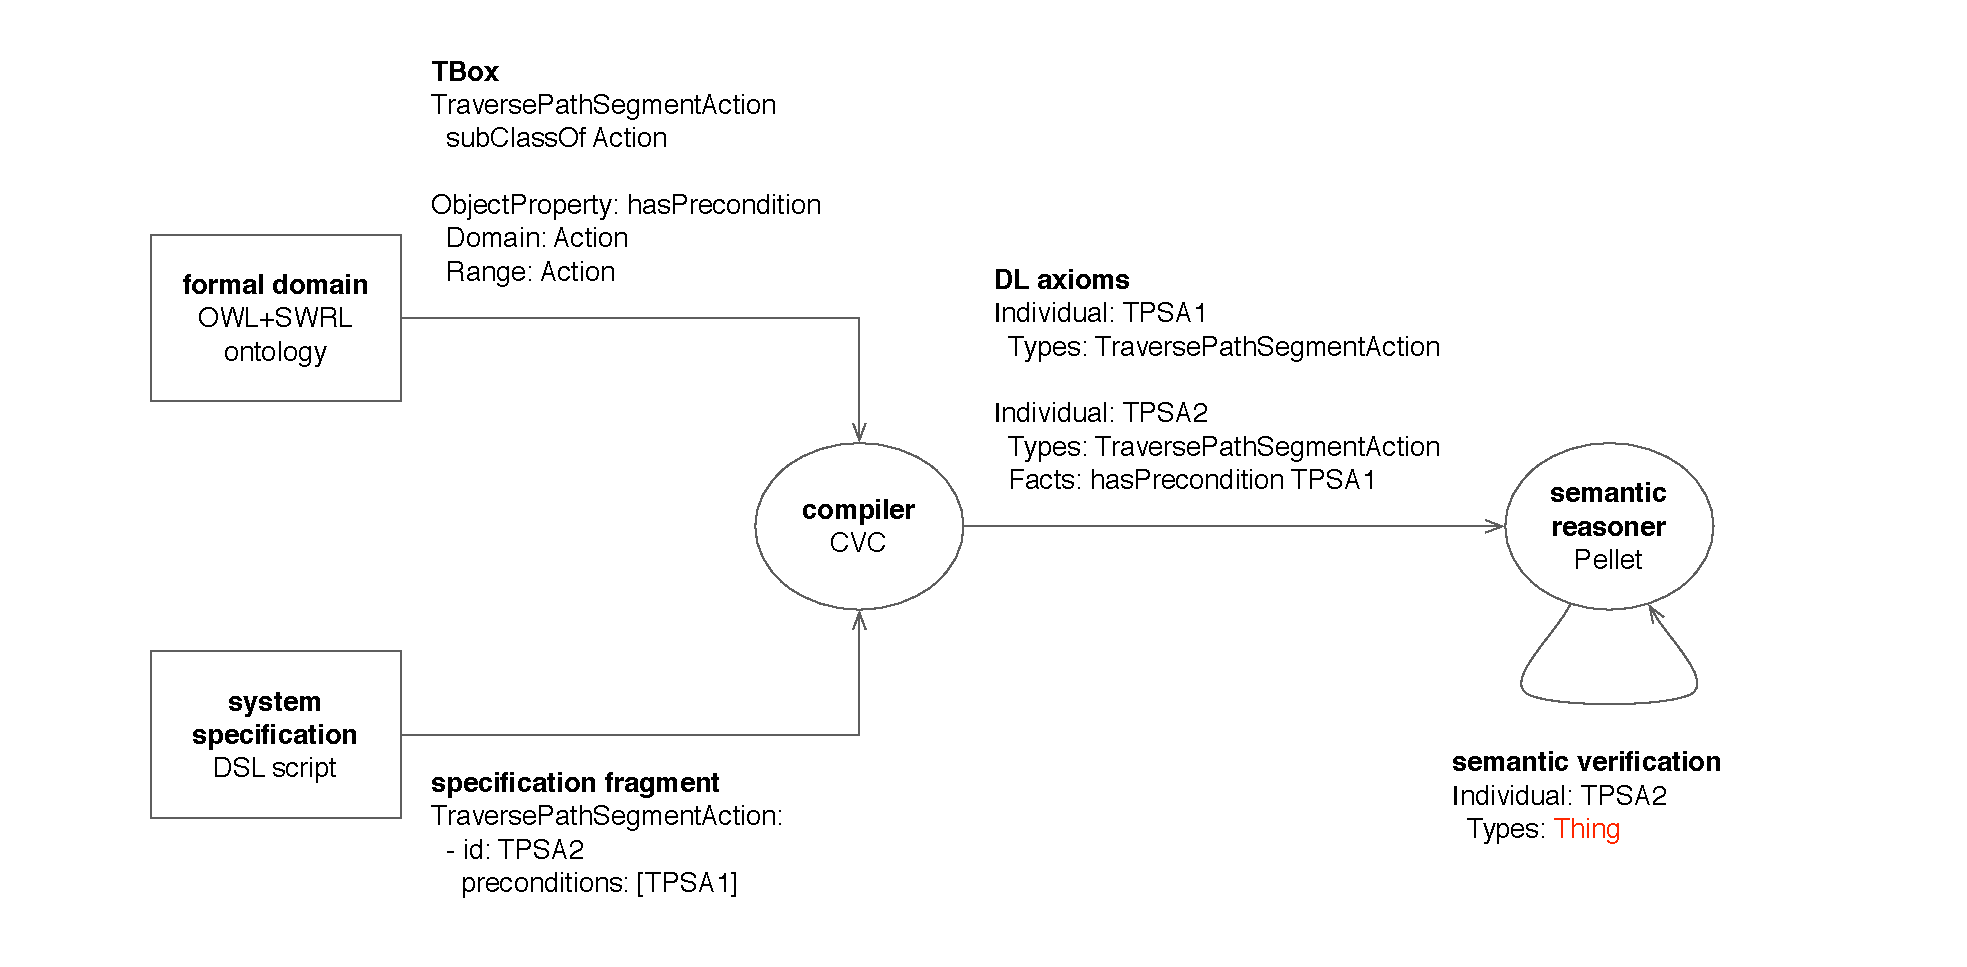
\includegraphics[width=\textwidth]{img/semantic-verification.pdf}
\caption[Semantic verification]{Elements of semantic verification with respect to the actions \texttt{TPSA1} and \texttt{TPSA2}, and the object property \texttt{hasPrecondition}.}
\label{fig:semantic_verification}
\end{figure}

With ABox consistency deduced, Pellet proceeds to generate inferences by, for example, reasoning about \emph{realization}, which determines the direct types of each individual. Realization-based inferences were described in Section~\ref{sec:Modeling_Tactical_Missions} with the classification of a specific kinetic action as a DTAA, and the resultant classification of the asset to which that action was assigned as a valid asset. As an example of realization with respect to Mission~A, let us assume a threat area action classification for action \texttt{TPSA4} (via the preprocessing phase described above). Given this assumption, Pellet would infer action \texttt{TPSA4} to be a DTAA because start point and endpoint of \texttt{TPSA4} are members of classes \texttt{Waypoint} (the start point of action \texttt{TPSA4} is the endpoint of action \texttt{TPSA3}, which is not a threat area action) and \texttt{ThreatAreaWaypoint}, respectively. Asset~\texttt{H2} would consequently be inferred a valid asset (since~\texttt{H2} executes at least one sensor action, namely \texttt{PSA5}, during the incursion).

Appendix~\ref{chap:Ontology} presents the generated ABox for Mission~A.

\section{Classification with Prolog}
\label{sec:Classification_with_Prolog}

Some Pellet inferences are transformed by the CVC into Prolog rules; for example, the Prolog rule \texttt{terminal} comprises knowledge inferred by Pellet (as described in Section~\ref{sec:Rule_Based_Modeling}). The Prolog code in Listing~\ref{lst:Prolog_rule_terminal_constrained_observer} formally defines rule \texttt{terminal\_constrain\-ed\_observer}, which encapsulates the atom \texttt{terminal}.

\begin{figure}[ht]
\begin{lstlisting}[caption={Prolog code for rule \texttt{terminal\_constrained\_observer}},label=lst:Prolog_rule_terminal_constrained_observer]
terminal_constrained_observer(X) :-
  constrained_observer(X),
  terminal(X).
\end{lstlisting}
\end{figure}

SWI-Prolog classifies each kinetic action with respect to the relationships that exist between it and other kinetic actions. For example, an action that is the last kinetic action to be executed by an asset, and has as precondition at least one cross-cutting kinetic action, is classified by SWI-Prolog as a \texttt{terminal\_constrained\_observer} (cross-cutting actions were introduced in Section~\ref{sec:Rule_Based_Modeling}). Figure~\ref{fig:composite_reasoning} illustrates elements of composite semantic- and Prolog-based reasoning with respect to the actions \texttt{TPSA1} and \texttt{TPSA2}; the inferred object property \texttt{isPreconditionTo} presented in Section~\ref{sec:Rule_Based_Modeling}; and the rule \texttt{terminal\_constrained\_observer}.

\begin{figure}[ht]
\centering
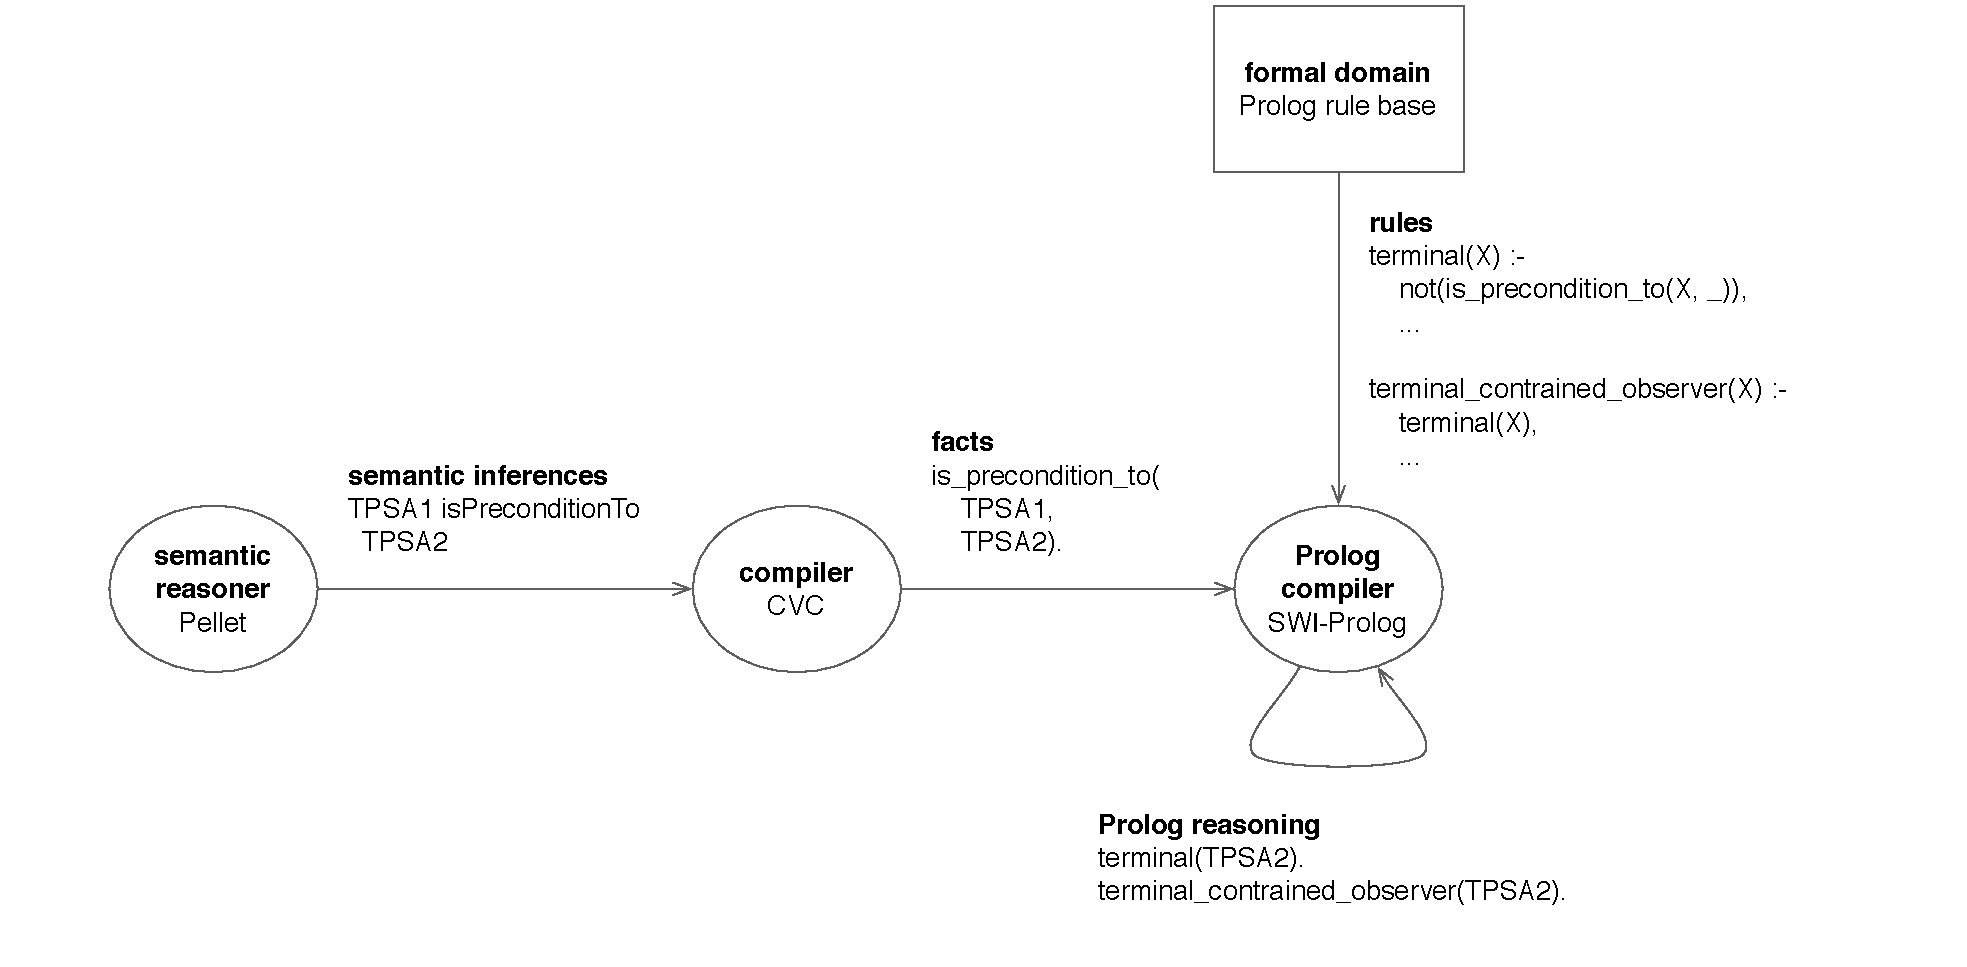
\includegraphics[width=\textwidth]{img/composite-reasoning.pdf}
\caption[Composite reasoning]{Elements of composite semantic- and Prolog-based reasoning with respect to the actions \texttt{TPSA1} and \texttt{TPSA2}; the inferred object property \texttt{isPreconditionTo} presented in Section~\ref{sec:Rule_Based_Modeling}; and the rule \texttt{terminal\_constrained\_observer}.}
\label{fig:composite_reasoning}
\end{figure}

The classification of a kinetic action affects the composition of the PRISM module for the asset to which that action is assigned; for example, the classification of action \texttt{TPSA2} in Mission~A as a \texttt{terminal\_constrained\_observer} affects the PRISM module corresponding to asset~\texttt{H1}. Affected asset module constructs include the action label of the command associated with \texttt{TPSA2} (recall that each asset module command is associated with a specific kinetic action) and, potentially, the action label of the last module command (see inferred arguments in Section~\ref{sec:Behavioral_Modeling}). Kinetic action classifications also generate mission properties; for example, as the last kinetic action to be executed by an asset, the successful execution of a \texttt{terminal\_constrained\_observer} is a desired mission property because it guarantees the successful execution of all preceding actions.

Table~\ref{tab:kinetic_action_classifications} highlights the impact of kinetic action classifications with respect to synthesized DTMC and PCTL constructs. For example, the action label of the asset module command associated with a \texttt{default} classification would assume the value of the identifier assigned to the classified action (as denoted by the dot notation); the action label of the command associated with a \texttt{terminal\_constrained\_observer} classification would assume the identifier of the asset to which the classified action is assigned; and, given the notation in Listing~\ref{lst:PCTL_action_duration_template}, the identifier of the property associated with a \texttt{terminal\_constrained\_observer} classification would assume the value of the identifier assigned to the classified action. Not applicable (n/a) and \texttt{null} values in Table~\ref{tab:kinetic_action_classifications} denote classifications that either do not affect the synthesis of a specific action label, or synthesize an empty action label, respectively. Thus Prolog inferences affect the synthesis of action labels, which in turn impact module synchronization (as described in Section~\ref{sec:Behavioral_Modeling}) and, ultimately, the verification results returned by PRISM\@.

\begin{sidewaystable}
	\centering
	\arrayrulecolor{Gray}
	\renewcommand*\arraystretch{1.3}
	\begin{tabular}{ l | l l | l }
		& \multicolumn{2}{ c | }{\textbf{DTMC asset module}} & \multicolumn{1}{ c }{\textbf{PCTL}}\\
		kinetic action classification & action label & last action label & property id\\
		\hline
		\texttt{default} & \texttt{action.id} & n/a & n/a\\
		\texttt{default\_singleton} & \texttt{action.id} & \texttt{null} & \texttt{action.id}\\
		\texttt{default\_terminal} & \texttt{action.id} & \texttt{null} & \texttt{action.id}\\
		\texttt{subject\_precondition} & \texttt{primary\_asset.id} & n/a & n/a\\
		\texttt{observer\_precondition} & \texttt{primary\_asset.id} & n/a & n/a\\
		\texttt{constrained\_subject} & \texttt{primary\_asset.id} & n/a & n/a\\
		\texttt{leading\_subject} & \texttt{action.id} & n/a & n/a\\
		\texttt{singleton\_subject} & \texttt{primary\_asset.id} & \texttt{primary\_asset.id} & n/a\\
		\texttt{terminal\_subject} & \texttt{primary\_asset.id} & \texttt{primary\_asset.id} & n/a\\
		\texttt{default\_observer} & \texttt{action.id} & n/a & n/a\\
		\texttt{terminal\_observer} & \texttt{action.id} & \texttt{null} & \texttt{action.id}\\
		\texttt{terminal\_constrained\_observer} & \texttt{action.asset.id} & \texttt{action.asset.id} & \texttt{action.id}\\
		\texttt{observer\_and\_constrained\_subject} & \texttt{primary\_asset.id} & n/a & n/a\\
		\texttt{observer\_and\_singleton\_subject} & \texttt{primary\_asset.id} & \texttt{primary\_asset.id} & n/a\\
		\texttt{observer\_and\_terminal\_subject} & \texttt{primary\_asset.id} & \texttt{primary\_asset.id} & n/a\\
		\texttt{subject\_constraint} & \texttt{primary\_asset.id} & n/a & n/a\\
		\texttt{terminal\_subject\_constraint} & \texttt{primary\_asset.id} & \texttt{primary\_asset.id} & \texttt{action.id}\\
	\end{tabular}
	\captionsetup{width=0.7\textwidth}
	\caption[Kinetic action classifications for DTMC and PCTL constructs]{Kinetic action classifications, which are ultimately derived via Prolog inferences, and their impact on synthesized DTMC and PCTL constructs associated with classified actions.}
	\label{tab:kinetic_action_classifications}
\end{sidewaystable}

For several kinetic action classifications, action labels assume the identifier of a \emph{primary asset} (as illustrated in Table~\ref{tab:kinetic_action_classifications}), which may be different from the asset to which a classified action is assigned. The behavioral modeling process described in Section~\ref{sec:Behavioral_Modeling} was guided by two concerns. Our primary goal was to develop template models and properties that could support the verification of multiple and variable UAV mission plans. It was also our intention to accurately model domain processes and thereby achieve the greatest possible confidence in the resulting verification process. To mimic real-world asset behavior, module executions were loosely coupled and synchronizations limited to occur on an as-needed basis. But this approach is not appropriate for modeling cross-cutting actions, which must be verified with temporal precision to ensure kinetic action workflow continuity during asset operations (this issue will be elaborated in Chapter~\ref{chap:Evaluation}). The conflict between modeling and analytical accuracy occurs because enabled DTMC commands are executed by PRISM with equal probability~\cite{PRISM_2010}. Lack of native scheduling precision necessitates the synchronization of all modules representing concepts related to cross-cutting actions. The required synchronization is achieved with the designation, via Prolog inferences, of a single primary asset whose identifier is assumed by the action labels associated with cross-cutting actions.

The Prolog code in Listing~\ref{lst:Prolog_rule_primary_asset} formally defines rule \texttt{primary\_asset}, which encapsulates inferred ontological knowledge encoded with the atoms \texttt{observer\_asset} (line~2), \texttt{observed\_asset} (line~4) and \texttt{observes} (lines~6 and~7). Rule \texttt{primary\_asset} formalizes the concept of a primary asset as an \emph{observer asset} (i.e., an asset observing other assets) that is either not itself observed by, or participates in a symmetric observer relationship with, another asset (a symmetric relationship is the opposite of the asymmetric relationship described in Section~\ref{sec:Modeling_Tactical_Missions}).

\begin{figure}[ht]
\begin{lstlisting}[caption={Prolog code for rule \texttt{primary\_asset}},label=lst:Prolog_rule_primary_asset]
primary_asset(A) :-
    observer_asset(A),
    (
        not(observed_asset(A));
        (
            observes(A, B),
            observes(B, A)
        (*)*)
    (*).*)
\end{lstlisting}
\end{figure}

Lines~1--3 in Listing~\ref{lst:OWL_class_ObserverAsset} formally define class \texttt{ObserverAsset}, which extends class \texttt{Asset}. Every member of class \texttt{ObserverAsset} must be associated via the object property \texttt{hasAction} with a member of class \texttt{Observer}. Lines~5 and~6 formally define the OWL class \texttt{Observer}, which is augmented by a synonymous SWRL rule (lines~8--13). Rule \texttt{Observer} formalizes the concept of an \emph{observer action} as an action that observes cross-cutting actions via preconditions. Given the domain knowledge encoded in Listing~\ref{lst:OWL_class_ObserverAsset}, an observer asset can be described more precisely as an asset that observes other assets via an assigned action that has as precondition a cross-cutting action. Conversely, an \emph{observed asset} is an asset observed by other assets via an assigned cross-cutting action. Class \texttt{ObservedAsset}, which formalizes the observed asset concept, is encoded in a similar manner to class \texttt{ObserverAsset}. Knowledge inferred by Pellet with respect to \texttt{ObserverAsset} and \texttt{ObservedAsset} is transformed by the CVC into knowledge encoded with the Prolog atoms \texttt{observer\_asset} and \texttt{observed\_asset}, respectively.

\begin{figure}[ht]
\begin{lstlisting}[caption={OWL+SWRL code for class \texttt{ObserverAsset}},label=lst:OWL_class_ObserverAsset]
Class: ObserverAsset
  EquivalentTo: Asset
    and (hasAction some Observer)

Class: Observer
  SubClassOf: Action

Rule:
    hasAction(?a, ?x),
    hasAction(?b, ?y),
    hasPrecondition(?y, ?x),
    DifferentFrom (?a, ?b)
  -> Observer(?y)
\end{lstlisting}
\end{figure}

Listing~\ref{lst:OWL_object_property_observes} formally defines the object property \texttt{observes} (lines~1--5), which is augmented by a synonymous SWRL rule (lines~7--12). Rule \texttt{observes} uses the cross-cutting action relationship (lines~8--11) to underpin an asset-oriented subject-observer relationship. Knowledge inferred by Pellet with respect to the OWL concept \texttt{observes} is transformed by the CVC into knowledge encoded with the Prolog atom \texttt{observes}, which is used in the context of rule \texttt{primary\_asset} to formalize a symmetric observer relationship. In conjunction with the observed and observer asset concepts, the \emph{observes} concept supports SWI-Prolog inferences with respect to \texttt{primary\_asset}, which in turn supports kinetic action classifications.

\begin{figure}[ht]
\begin{lstlisting}[caption={OWL+SWRL code for the object property \texttt{observes}},label=lst:OWL_object_property_observes]
ObjectProperty: observes
  Characteristics: Asymmetric,
    Irreflexive
  Domain: Asset
  Range: Asset

Rule:
    hasAction(?a, ?x),
    hasAction(?b, ?y),
    hasPrecondition(?y, ?x),
    DifferentFrom (?a, ?b)
  -> observes(?a, ?b)
\end{lstlisting}
\end{figure}

Rule \texttt{primary\_asset} enables Prolog to discover the assets with assigned cross-cutting actions that have temporal precedence in a workflow of related actions. Such a workflow may comprise one or, given the symmetric observer relationship encapsulated in \texttt{primary\_asset}, multiple primary assets. The action label identifier resulting from a single primary asset guarantees the synchronization of all modules representing concepts related to cross-cutting actions. Synchronization is also guaranteed with multiple primary assets when a single identifier is chosen randomly from the candidate set. We note that a single mission plan comprising multiple independent action workflows could be verified by PRISM without the need for synchronization between the actions that constitute those workflows.

The primary asset mechanism may be perceived as an obfuscated method for achieving what is in essence a random result, at least with respect to a subset of the mission space. But primary assets support an inference-based selection process that is conceptually compatible with the methods that derive the remaining action- and asset-based identifiers in Table~\ref{tab:kinetic_action_classifications}. And while this mechanism fails to eliminate randomness during the identifier selection process, it performs better than random by eliminating and minimizing randomness for mission plans comprising one or more primary assets, respectively. It is of course entirely possible for the primary asset concept, and the reasoning that it affords, to be extended or repurposed in subsequent versions of our prototype. In any case, these concerns apply neither to our method nor our prototype as a whole, but rather to a small subset of the domain model that constitutes our prototype.

As a prelude to the following section, which presents synthesized PRISM artifacts, Table~\ref{tab:Mission_A_classifications} lists kinetic action classifications for the path segment traversal actions specified in Mission~A (top), and the impact of each classification on the synthesized DTMC and PCTL constructs associated with the classified action (bottom).

\newcommand{\true}{\textcolor{green}{true}}
\newcommand{\false}{\textcolor{red}{false}}

\begin{table}[ht]
	\arrayrulecolor{Gray}
	\renewcommand*\arraystretch{1.3}
	\begin{tabularx}{\textwidth}{
			>{\raggedright\hsize=0.56\hsize}X|
			>{\centering\hsize=0.11\hsize}X
			>{\centering\hsize=0.11\hsize}X
			>{\centering\hsize=0.11\hsize}X
			>{\centering\hsize=0.11\hsize}X
		}
		& \texttt{TPSA1} & \texttt{TPSA2} & \texttt{TPSA3} & \texttt{TPSA4}\tabularnewline
		\hline
		\texttt{default} & \false & \false & \false & \false\tabularnewline
		\texttt{default\_singleton} & \false & \false & \false & \false\tabularnewline
		\texttt{default\_terminal} & \false & \false & \false & \false\tabularnewline
		\texttt{subject\_precondition} & \false & \false & \false & \false\tabularnewline
		\texttt{observer\_precondition} & \true & \false & \false & \false\tabularnewline
		\texttt{constrained\_subject} & \false & \false & \true & \false\tabularnewline
		\texttt{leading\_subject} & \false & \false & \false & \false\tabularnewline
		\texttt{singleton\_subject} & \false & \false & \false & \false\tabularnewline
		\texttt{terminal\_subject} & \false & \false & \false & \false\tabularnewline
		\texttt{default\_observer} & \false & \false & \false & \false\tabularnewline
		\texttt{terminal\_observer} & \false & \false & \false & \false\tabularnewline
		\texttt{terminal\_constrained\_observer} & \false & \true & \false & \false\tabularnewline
		\texttt{observer\_and\_constrained\_subject} & \false & \false & \false & \false\tabularnewline
		\texttt{observer\_and\_singleton\_subject} & \false & \false & \false & \false\tabularnewline
		\texttt{observer\_and\_terminal\_subject} & \false & \false & \false & \false\tabularnewline
		\texttt{subject\_constraint} & \false & \false & \false & \false\tabularnewline
		\texttt{terminal\_subject\_constraint} & \false & \false & \false & \true\tabularnewline
		\hline\hline
		asset module action label & \texttt{H1} & \texttt{H1} & \texttt{H1} & \texttt{H1}\tabularnewline
		asset module last action label & n/a & \texttt{H1} & n/a & \texttt{H1}\tabularnewline
		property id & n/a & \texttt{TPSA2} & n/a & \texttt{TPSA4}\tabularnewline
	\end{tabularx}
	\caption[Kinetic action classifications for Mission~A]{Kinetic action classifications for the path segment traversal actions specified in Mission~A (top), and the impact of each classification on the synthesized DTMC and PCTL constructs associated with the classified action (bottom).}
	\label{tab:Mission_A_classifications}
\end{table}

\section{Synthesized Models and Properties}
\label{sec:Synthesized_Models_and_Properties}

The CVC uses explicit and inferred domain knowledge to synthesize DTMC and PCTL artifacts from predefined templates; for example, the asset module template presented in Section~\ref{sec:Behavioral_Modeling} underpins the synthesis of one module per each asset in Mission~A\@. The PRISM code in Listing~\ref{lst:PRISM_asset_module_code} specifies a synthesized asset module corresponding to asset~\texttt{H2}, where the commands in lines~3 and~4 represent, respectively, the execution of actions~\texttt{TPSA3} and~\texttt{TPSA4} assigned to~\texttt{H2}.

\begin{figure}[ht]
\begin{lstlisting}[caption={PRISM asset module code},label=lst:PRISM_asset_module_code]
module Hummingbird2
  e2 : [0..120] init 120;
  [H1] e2>0 & d3>0 -> (e2'=e2-1);
  [H1] e2>0 & d4>0 -> (e2'=e2-1);
  [H1] e2=0 | d4=0 -> true;
endmodule
\end{lstlisting}
\end{figure}

As a consequence of the realization-based inferences described in Section~\ref{sec:Verification_with_Semantic_Reasoning}, the CVC synthesizes an asset survivability module to calculate the probability of survival for~\texttt{H2} (as described in Section~\ref{sec:Modeling_Survivability}). The PRISM code in Listing~\ref{lst:PRISM_asset_survivability_code} specifies the synthesized survivability module corresponding to asset~\texttt{H2}, where variable~\texttt{a2d} (lines~6--8) represents the asset's destruction.

\begin{figure}[ht]
\begin{lstlisting}[caption={PRISM asset survivability code},label=lst:PRISM_asset_survivability_code]
const int start4 = 60;
const int finish4 = 0;
formula actn4_tai = d4>finish4 & d4<=start4;

module Hummingbird2_Survivability
  a2d : bool init false;
  [H1] !a2d & (*\hspace{1.8mm}*)actn4_tai -> 0.99:(a2d'=false) + 0.01:(a2d'=true);
  [H1] (*\hspace{1.8mm}*)a2d | !actn4_tai -> true;
endmodule
\end{lstlisting}
\end{figure}

The CVC also synthesizes PRISM code to calculate a RAF value for the threat area incursion prosecuted by asset~\texttt{H2} (as described in Section~\ref{sec:Modeling_Risk_Acceptability}). The PRISM code in Listing~\ref{lst:PRISM_risk_acceptability} specifies the synthesized sensor action counter module corresponding to asset~\texttt{H2}. Variables \texttt{start4}, \texttt{finish4} and \texttt{actn4\_tai} in Listing~\ref{lst:PRISM_risk_acceptability} are declared in Listing~\ref{lst:PRISM_asset_survivability_code}.

\begin{figure}[ht]
\begin{lstlisting}[caption={PRISM risk acceptability code},label=lst:PRISM_risk_acceptability]
formula duration4 = start4 - finish4;

formula tkad2 = duration4;

module SensorActionCounter2
  sad2 : [0..tkad2] init 0;
  [H1] (*\hspace{1.8mm}*)actn4_tai &(*\hspace{1.8mm}*) (r5) & sad2<tkad2 -> (sad2'=sad2+1);
  [H1] !actn4_tai | !(r5) -> true;
endmodule

formula raf2 = sad2 / tkad2;
\end{lstlisting}
\end{figure}

At the conclusion of the synthesis process, the DTMC artifact that models Mission~A is verified against a set of synthesized PCTL properties. The PRISM code in Listing~\ref{lst:PRISM_mission_property} specifies a synthesized property for Mission~A\@. This property comprises variables~\texttt{d2} and~\texttt{d4}, which represent the durations of~\texttt{TPSA2} and~\texttt{TPSA4}, respectively; variable \texttt{a2d}, described above; and variable~\texttt{raf2}, which represents the RAF value for the threat area incursion committed by asset~\texttt{H2}. The property need not comprise variables to represent the durations of~\texttt{TPSA1} and~\texttt{TPSA3} because these actions precede~\texttt{TPSA2} and~\texttt{TPSA4}, respectively. In other words, the successful execution of~\texttt{TPSA1} is implied by the successful execution of~\texttt{TPSA2} (this implication is denoted by the classification of \texttt{TPSA2} as a \texttt{terminal\_constrained\_observer}), etc.

\begin{figure}[ht]
\begin{lstlisting}[caption={PRISM mission property code},label=lst:PRISM_mission_property]
P=? [ F d2=0 & d4=0 & !a2d & raf2>0.6(*\hspace{1.8mm}*)]
\end{lstlisting}
\end{figure}

Given the property in Listing~\ref{lst:PRISM_mission_property}, the probability of success for Mission~A is calculated by PRISM to be approximately 0.299. In particular, the verification of Mission~A assigns variables~\texttt{d2} and~\texttt{d4} with values of zero; variable~\texttt{!a2d} is assigned a probability of approximately 0.299; and variable~\texttt{raf2} is assigned a value of approximately 0.833.

\section{Implementation}
\label{sec:Implementation}

We have implemented several of the components that constitute our prototype. The ontology described in Section~\ref{sec:Semantic_Modeling} and Section~\ref{sec:Rule_Based_Modeling} was implemented in OWL+SWRL\@. The Prolog rule-base described in Section~\ref{sec:Rule_Based_Modeling} was implemented in SWI-Prolog. The DTMC and PCTL templates presented in Section~\ref{sec:Behavioral_Modeling} were implemented in the programming language Ruby (version 1.9.3). And the DSL described in Section~\ref{sec:High_Level_Specifications_in_YAML} was implemented in YAML, which is particularly compatible with Ruby. Because of its powerful reflective and meta-programming capabilities, Ruby affords our prototype flexibility to substitute the current YAML DSL with a more expressive mission specification language, if so required~\cite{Flanagan_2008,Perrotta_2010}.

In developing the prototype, we leveraged open source software including Pellet 2.2.0, PRISM 4.1 and the Prot\'{e}g\'{e} ontology editor (version 4.1.0). While integration, testing and extension of implemented components is currently ongoing, completed work was sufficient to support an evaluation, which is presented in Chapter~\ref{chap:Evaluation}.

\section{Related Work}
\label{sec:Cascading_Verification_Related_Work}

Cascading verification can be considered a form of semantic model checking, which has been studied exclusively in the context of the Web service domain.

Narayanan and McIlraith encode Web service capability descriptions and behavioral properties with DAML-S and Petri net formalisms, respectively~\cite{Narayanan_2002}. DAML-S is a DAML+OIL ontology for describing Web services. For any given Web service, an implemented system generates the Petri net corresponding to the DAML-S description of that service. The resulting net is used by KarmaSIM, a modeling and simulation environment, to perform various analysis techniques including reachability analysis and deadlock detection.

The model checking algorithm presented by Di Pietro et al.\ uses a DL-based ontology to formalize the Web service domain~\cite{Di_Pietro_2012}. The behavior of each Web service is modeled as a \emph{state transition system} (STS), while behavioral requirements are encoded with CTL\@. Both STS and CTL formalisms are extended with semantic annotations. For any given Web service, the algorithm generates a finite STS corresponding to the annotated description of that service. The resulting model is verified with model checking. The same algorithm is used by Boaro et al.\ to verify Web service security requirements~\cite{Boaro_2010}.

Oghabi et al.\ use OWL-S, an OWL ontology that supersedes DAML-S, to describe Web service behavior~\cite{Oghabi_2011}. For any given Web service, an implemented system generates a PRISM model corresponding to the OWL-S description of that service. The resulting model is verified with PRISM\@. Ankolekar et al.\ translate OWL-S process models to equivalent PROMELA models, which are verified with the SPIN model checker~\cite{Ankolekar_2005}. Liu et al.\ extend OWL-S with multiple annotation layers for specifying Web service flow properties including temporal constraints~\cite{Liu_2008}. Annotated OWL-S models are transformed to corresponding \emph{time constraint Petri net} (TCPN) models, which are verified with model checking. Lomuscio and Solanki express OWL-S process models with the \emph{interpreted systems programming language} (ISPL)~\cite{Lomuscio_2009}. ISPL is the system description language for MCMAS, a symbolic model checker tailored to the verification of multi-agent systems. In this context, Web services and Web service compositions are viewed as agents and multi-agent systems, respectively.

Our method is perhaps most compatible with the work presented by Oghabi et al. Similarities include the motivation to verify stochastic behavior and the development of a system that synthesizes PRISM models from OWL knowledge. But unlike our prototype, the system developed by Oghabi et al.\ does not synthesize behavioral properties, nor does it exploit inferred knowledge to support the synthesis of DTMC artifacts. Inferred knowledge is utilized in other work including that of Narayanan and McIlraith, Di Pietro et al.\ and Boaro et al. But existing work is exclusively concerned with the verification of Web services, and does not address the expressive and reasoning limitations that constrain OWL\@. The work presented in this thesis is (to our knowledge) unique because it addresses semantic model checking limitations, and applies the resulting method to a novel domain.

\section{Summary}
\label{sec:Cascading_Verification_Summary}

Chapter~\ref{chap:Domain_Modeling} describes the technologies and modeling methods that underpin cascading verification; in this chapter, we describe the actual verification process, which involves several stages of reasoning and analysis. The process begins when model builders use a high-level DSL to encode system specifications. A compiler uses automated reasoning to verify the consistency between each specification and formalized domain knowledge encoded in OWL+SWRL and Prolog. If consistency is deduced, then explicit and inferred domain knowledge is used by the compiler to synthesize a system model and behavioral properties from template code. PRISM subsequently verifies the model against the properties.

At its core, this chapter exposes the composite inference mechanism that underpins our method and prototype. Composite reasoning encompasses Pellet- and Prolog-based inference services; the former include consistency checking and realization with respect to an OWL+SWRL ontology, while the latter involve query resolution with respect to a knowledge base comprising rules and facts. Prolog-based inferences enable our prototype to classify kinetic actions, and thereby calibrate the synthesis of PRISM modules related to those actions. Our implementation of composite reasoning is illustrated with several examples in the context of Mission~A, which is assumed to involve the prosecution of a threat area incursion. The discussion in this chapter thus utilizes the tactical case study introduced in Section~\ref{sec:Modeling_Tactical_Missions}.

By tracing cascading verification from system specifications to probabilistic model checking, we describe a prototype greater than the sum of its parts, i.e., a prototype that integrates technologies presented in Chapter~\ref{chap:Domain_Modeling} to improve the correctness of UAV mission plans. The following chapter quantifies this improvement.

\chapter{Evaluation}
\label{chap:Evaluation}

We assert that by enhancing the abstraction level of model and property specifications, cascading verification also enhances the effectiveness of probabilistic model checking. To validate this assertion, we will demonstrate that, as an implementation of cascading verification for the UAV domain, the prototype presented in this thesis benefits mission developers by simplifying the verification of UAV mission plans, and by augmenting PRISM's verification capabilities. Ultimately, we aim to show that our prototype benefits mission developers by improving the correctness of UAV mission specifications. We will also evaluate the portability of cascading verification, i.e., the usability of our method in the context of different application domains.

The remainder of this chapter is structured as follows. Section~\ref{sec:Evaluation_Methods_and_Metrics} describes the methodologies and metrics that underpin the evaluation of our method and prototype. Limitations and threats to the validity of the evaluation are presented in Section~\ref{sec:Threats_to_Validity}. This chapter is summarized in Section~\ref{sec:Evaluation_Summary}.

\section{Evaluation Methods and Metrics}
\label{sec:Evaluation_Methods_and_Metrics}

This evaluation focuses on a single project, and assesses the effects of change prior to large-scale implementation and deployment. Case studies therefore constitute an appropriate evaluation method~\cite{Kitchenham_1995}. Importantly, case studies 1) avoid scalability issues associated with the evaluation of software-engineering tools and methods, and 2) support high-level assessments, which are desirable for wide-ranging process changes. The evaluation was not affected by ancillary budgetary, scheduling and staffing issues.

\subsection{Abstraction}

Because it was unfeasible to involve practitioners in the evaluation of our prototype's utility, we opted instead for a metrics-based analysis of~58 mission plans. These plans were based on real-world mission scenarios developed independently by DARPA and DRDC~\cite{DARPA,Youngson_2004}. We evaluated our approach by comparing the LOC and numbers of lexical tokens required to specify missions in YAML against the LOC and tokens in the combined DTMC and PCTL code synthesized by the CVC\@. On average, our prototype synthesizes PRISM code that is 3.127 and 4.490 times greater than the size of YAML input with regard to LOC and tokens, respectively. (The standard deviations were 52.4\% and 95.4\%, respectively.) These results provide preliminary evidence of non-trivial reduction in the effort required to produce mission models and properties.

Table~\ref{tab:mission_metrics} lists metric values for a subset of the~58 mission plans. This subset represents the full range of observed PRISM-to-YAML ratios. (Appendix~\ref{chap:Mission_Verification_Artifacts} contains verification artifacts---including mission specifications encoded in YAML, synthesized DTMC and PCTL artifacts, and PRISM results---for the mission plans presented in Table~\ref{tab:mission_metrics}.)

\begin{table}[ht]
	\arrayrulecolor{Gray}
	\renewcommand*\arraystretch{1.3}
	\begin{tabularx}{\textwidth}{
			>{\centering\hsize=0.08\hsize}X|
			>{\centering\hsize=0.14\hsize}X
			>{\centering\hsize=0.14\hsize}X|
			>{\centering\hsize=0.14\hsize}X
			>{\centering\hsize=0.14\hsize}X|
			>{\centering\hsize=0.18\hsize}X
			>{\centering\hsize=0.18\hsize}X
		}
		& \multicolumn{2}{ c | }{YAML} &
			\multicolumn{2}{ c | }{PRISM} &
			\multicolumn{2}{ c }{PRISM-to-YAML ratio}\tabularnewline
		id & LOC & tokens & LOC & tokens & LOC & tokens\tabularnewline
		\hline
		1a & 9 & 31 & 22 & 104 & 244.4\% & 335.5\%\tabularnewline
		1d & 12 & 45 & 32 & 169 & 266.7\% & 375.6\%\tabularnewline
		1g & 15 & 59 & 36 & 218 & 240.0\% & 369.5\%\tabularnewline
		2a & 18 & 70 & 45 & 255 & 250.0\% & 364.3\%\tabularnewline
		2b & 18 & 72 & 52 & 277 & 288.9\% & 384.7\%\tabularnewline
		2e & 23 & 97 & 57 & 331 & 247.8\% & 341.2\%\tabularnewline
		2g & 25 & 105 & 77 & 457 & 308.0\% & 435.2\%\tabularnewline
		2j & 23 & 98 & 76 & 443 & 330.4\% & 452.0\%\tabularnewline
		2m & 26 & 112 & 91 & 558 & 350.0\% & 498.2\%\tabularnewline
		2p & 26 & 114 & 91 & 562 & 350.0\% & 493.0\%\tabularnewline
		2r & 25 & 109 & 84 & 468 & 336.0\% & 429.4\%\tabularnewline
		2u & 28 & 123 & 94 & 533 & 335.7\% & 433.3\%\tabularnewline
		2v & 28 & 123 & 99 & 583 & 353.6\% & 474.0\%\tabularnewline
		2w & 31 & 137 & 111 & 666 & 358.1\% & 486.1\%\tabularnewline
		2x & 31 & 137 & 111 & 666 & 358.1\% & 486.1\%\tabularnewline
		3a & 12 & 42 & 32 & 158 & 266.7\% & 376.2\%\tabularnewline
		3e & 15 & 56 & 45 & 252 & 300.0\% & 450.0\%\tabularnewline
		3h & 16 & 61 & 42 & 227 & 262.5\% & 372.1\%\tabularnewline
		3k & 18 & 70 & 60 & 357 & 333.3\% & 510.0\%\tabularnewline
		3o & 18 & 72 & 60 & 373 & 333.3\% & 518.1\%\tabularnewline
		4a & 21 & 94 & 39 & 267 & 185.7\% & 284.0\%\tabularnewline
		4b & 21 & 94 & 73 & 513 & 347.6\% & 545.7\%\tabularnewline
		4d & 25 & 110 & 100 & 707 & 400.0\% & 642.7\%\tabularnewline
		4f & 28 & 124 & 111 & 788 & 396.4\% & 635.5\%\tabularnewline
		5a & 23 & 92 & 58 & 329 & 252.2\% & 357.6\%\tabularnewline
		5b & 23 & 92 & 104 & 744 & 452.2\% & 808.7\%\tabularnewline
	\end{tabularx}
	\caption[Mission plan metric values]{Metric values for representative mission plans.}
	\label{tab:mission_metrics}
\end{table}

We observe that tactical missions (4b, 4d and~4f in Table~\ref{tab:mission_metrics}) and traffic surveillance missions (5a and~5b) generate more LOC and tokens than \emph{standalone mission plans}, which are mission plans underpinned exclusively by CEMO and thereby not associated with the more specialized subdomains encoded in Tactical- and Traffic-CEMO\@. Specifically, tactical mission plans generate PRISM code that is on average 3.933 and 5.992 times greater than the size of YAML input with regard to LOC and tokens, respectively. (The standard deviations were 24.0\% and 59.2\%, respectively.) Mission~5b generates PRISM code that is 4.522 and 8.087 times greater than the size of YAML input with regard to LOC and tokens, respectively. Because the effort required to synthesize PRISM code is proportional to the effort required to synthesize the LOC and tokens that constitute the code, tactical and traffic surveillance mission plans result in added value for mission developers. This observation suggests that, with respect to tactical missions, the utility of our prototype is proportional to the threat level associated with any given mission plan. More broadly, increased LOC and token output suggests that the utility of cascading verification may be proportional to the amount of automated reasoning required to synthesize pertinent artifacts, a conclusion that justifies our motivation to augment model checking with formalized domain knowledge.

\subsection{Effectiveness}

Because it cannot account for the intricate syntax of the PRISM language, a LOC- and token-based analysis offers limited insight into the inherent complexity of model and property specifications. We investigate complexity further by considering \emph{behavioral modeling errors} specific to the PRISM language that can be eliminated with the automated synthesis of PRISM artifacts (at least for the segment of the mission space that we have explored thus far). These errors are significant, perhaps more so than the errors uncovered during the model checking process, because they can mislead mission developers by causing PRISM to verify erroneous mission plans.

In the context of the PRISM language and the PRISM models created for this project:

\begin{itemize}

\item\emph{Inconsistent variable errors} occur when PRISM variables are inconsistent in value with corresponding variables in mission specifications; for example, the duration of an action specified in YAML should be consistent in value with the local variable of the PRISM module corresponding to that action.\footnote{Action duration in the context of behavioral modeling was described in Section~\ref{sec:Behavioral_Modeling}.}

\item\emph{Command action errors} occur when command actions, which affect module synchronization, are incorrect across two or more modules.

\item\emph{Command probability errors} occur when commands are annotated with probabilities that fail to accurately reflect the system being modeled; for example, the probabilities encapsulated in an asset survivability module should accurately reflect the vulnerability of the asset corresponding to that module.\footnote{Asset survivability was described in Section~\ref{sec:Modeling_Tactical_Missions}.}

\item\emph{Command update errors} occur when command updates, which affect module behavior, are incomplete or incorrect. For example, an incomplete update could fail to couple the modules corresponding to an asset and the action assigned to that asset; an incorrect update could couple modules corresponding to an asset and an action assigned to a different asset.

\end{itemize}

We also consider mission specification errors that are beyond the scope of PRISM's verification capabilities. These \emph{domain-specific errors} are detected by either Pellet or the SWI-Prolog compiler during the synthesis process. We have identified 28 domain-specific errors, across six error classes, that impact the correctness of UAV missions. In the context of the OWL language and CEMO:

{
\parindent=0em

\newcommand{\myindent}[1]{\hangindent=2em\emph{#1}}

\myindent{Disjoint class errors} occur when individuals are declared in system specifications to be instances of incompatible classes; for example, a hover action can also be a kinetic action, but not a sensor action. This error type affects mission correctness by ambiguating mission constructs for humans and, potentially, computers. Construct ambiguity could, for example, cause humans to confuse action subtypes and thereby develop mission plans comprising one or more sensor actions and zero kinetic actions; without appropriate verification, automated processes could subsequently attempt to deploy erroneous missions that violate asset constraints related to the execution of kinetic actions (as described in Section~\ref{sec:Semantic_Modeling}). The OWL statements in Listing~\ref{lst:disjoint_classes} formally define disjoint classes that can cause domain-specific errors.

\begin{lstlisting}[caption={Disjoint class statements specified in OWL},label=lst:disjoint_classes]
Action DisjointWith Asset
ARDrone DisjointWith Hummingbird
HoverAction DisjointWith TraversePathSegmentAction
HoverAction DisjointWith LidarAction
HoverAction DisjointWith PhotoSurveillanceAction
TraversePathSegmentAction DisjointWith LidarAction
TraversePathSegmentAction DisjointWith PhotoSurveillanceAction
LidarAction DisjointWith PhotoSurveillanceAction
\end{lstlisting}

\myindent{Existential restriction errors} occur when individuals fail to participate in mandatory relationships, as specified by the OWL keyword \texttt{some}; for example, every asset must execute at least one kinetic action. The OWL statements in Listing~\ref{lst:existential_restrictions_in_OWL} formally define existential restrictions that can cause domain-specific errors. Because of OWA, which was described in Section~\ref{sec:OWL_SWRL_and_Prolog}, OWL-based reasoning cannot conclude the absence of a mandatory relationship from the absence of knowledge about that relationship. Consequently, existential restriction errors are detected exclusively by the SWI-Prolog compiler. The Prolog rules in Listing~\ref{lst:existential_restrictions_in_Prolog} encompass atoms that correspond to the existential restrictions in Listing~\ref{lst:existential_restrictions_in_OWL}.

\begin{figure}[ht]
\begin{lstlisting}[caption={Existential restriction statements specified in OWL},label=lst:existential_restrictions_in_OWL]
Asset hasAction some KineticAction
Asset hasEnduranceInSeconds some int
HoverAction hasWaypoint some Waypoint
KineticAction hasDurationInSeconds some int
LidarAction hasIntervalInSeconds some int
LidarAction isConcurrentWith some HoverAction
Mission hasAsset some Asset
PhotoSurveillanceAction hasDurationInSeconds some int
TraversePathSegmentAction hasEndpoint some Waypoint
TraversePathSegmentAction hasStartPoint some Waypoint
\end{lstlisting}
\end{figure}

\begin{figure}[ht]
\begin{lstlisting}[caption={Existential restrictions encompassed in Prolog rules},label=lst:existential_restrictions_in_Prolog]
invalid_asset(A) :-
    zero_action_asset(A);
    not(has_endurance_in_seconds(A, _)).

invalid_hover_action(H) :-
    invalid_kinetic_action(H);
    not(has_waypoint(H, _)).

invalid_kinetic_action(K) :-
    not(has_duration_in_seconds(K, _)).

invalid_lidar_action(L) :-
    not(has_interval_in_seconds(L, _));
    not(is_concurrent_with(L, _)).

invalid_mission(M) :-
    not(has_asset(M, _)).

invalid_photo_surveillance_action(P) :-
    not(has_duration_in_seconds(P, _)).

invalid_traverse_path_segmentAction(T) :-
    invalid_kinetic_action(T);
    not(has_endpoint(T, _));
    not(has_start_point(T, _)).
\end{lstlisting}
\end{figure}

\myindent{Data property value errors} occur when data property values declared in system specifications fall outside the ranges of corresponding data properties encoded in CEMO; for example, the endurance of a Hummingbird is 1200 time-steps. The OWL statements in Listing~\ref{lst:data_property_values} formally define data properties that can cause domain-specific errors.

\begin{figure}[ht]
\begin{lstlisting}[caption={Data property statements specified in OWL},label=lst:data_property_values]
ARDrone hasEnduranceInSeconds some int[<= 70]
Hummingbird hasEnduranceInSeconds some int[<= 120]
\end{lstlisting}
\end{figure}

\myindent{Data property domain and range errors} occur when data property domain and range types declared in system specifications are inconsistent with the domain and range types of the corresponding data properties encoded in CEMO; for example, CEMO specifies that every \texttt{Hummingbird} individual must be associated with a datatype property \texttt{hasCostValue} of type \texttt{int}. The OWL code in Listing~\ref{lst:data_properties} formally defines data properties that can cause domain-specific errors.

\begin{figure}[ht]
\begin{lstlisting}[caption={Data properties specified in OWL},label=lst:data_properties]
DataProperty: hasDurationInSeconds
  Characteristics: Functional
  Domain: Action
  Range: int

DataProperty: hasEnduranceInSeconds
  Characteristics: Functional
  Domain: Asset
  Range: int

DataProperty: hasIntervalInSeconds
  Characteristics: Functional
  Domain: LidarAction
  Range: int
\end{lstlisting}
\end{figure}

\myindent{Object property domain and range errors} occur when object property domain and range types declared in system specifications are inconsistent with the domain and range types of the corresponding object properties encoded in CEMO; for example, CEMO specifies that the object property \texttt{hasAction} associates every member of class \texttt{Asset} (the domain of \texttt{hasAction}) with a member of class \texttt{KineticAction} (the range). The OWL code in Listing~\ref{lst:object_properties} formally defines object properties that can cause domain-specific errors.

\begin{figure}[ht]
\begin{lstlisting}[caption={Object properties specified in OWL},label=lst:object_properties]
ObjectProperty: hasAction
  Characteristics: Asymmetric, Irreflexive, InverseFunctional
  Domain: Asset
  Range: Action
  InverseOf: isActionOf

ObjectProperty: hasAsset
  Characteristics: Asymmetric, Irreflexive, InverseFunctional
  Domain: Mission
  Range: Asset

ObjectProperty: hasPrecondition
  Characteristics: Transitive
  Domain: Action
  Range: Action
  InverseOf: isPreconditionTo

ObjectProperty: isConcurrentWith
  Characteristics: Asymmetric, Irreflexive
  Domain: LidarAction
  Range: HoverAction
\end{lstlisting}
\end{figure}

\myindent{Threatened asset errors} occur when mission plans comprise a threatened asset that is not also a valid asset.\footnote{Threatened and valid assets were described in Section~\ref{sec:Modeling_Tactical_Missions}.} With the exception of this UAV-related error class, domain-specific errors are caused by inconsistencies between a mission specification and the underlying domain model. Given adequate documentation of the YAML DSL, these inconsistencies could, in theory, be eliminated by mission developers during the design and implementation of mission plans (in practice, software bugs elude extinction). But threatened and valid assets can only be discovered with geodetic calculations and subsequent formal reasoning, as described in Section~\ref{sec:From_Specification_to_Verification} and Section~\ref{sec:Modeling_Tactical_Missions}, respectively. The OWL code in Listing~\ref{lst:OWL_class_ThreatenedAsset} formally defines class \texttt{ThreatenedAsset}.

}

\begin{figure}[ht]
\begin{lstlisting}[caption={OWL code for class \texttt{ThreatenedAsset}},label=lst:OWL_class_ThreatenedAsset]
Class: ThreatenedAsset
  EquivalentTo: Asset
    and (hasAction some DirectThreatAreaHoverAction)
  DisjointWith: DirectThreatAreaTPSA
\end{lstlisting}
\end{figure}

Mission correctness can clearly be compromised by domain-specific and behavioral modeling errors, which occur during the design/implementation and verification phases, respectively, of the mission development process. Our prototype augments PRISM's effectiveness by preventing both of these error types.

\subsection{Probabilistic Verification}

Finally, we consider PRISM's ability to meaningfully verify UAV mission plans (or rather, we consider the utility of the DTMC and PCTL artifacts synthesized by our prototype). For this part of the evaluation, eighteen of the~58 mission plans described above were seeded with errors, including deadlock and non-reachable states, that violated desirable behavioral properties. One mission plan failed (i.e., contained errors that resulted in a 0.0 probability of success) because of an unacceptably low RAF value.\footnote{The RAF value was described in Section~\ref{sec:Verification_with_Semantic_Reasoning}.}

Nine mission plans failed because kinetic or sensor action workflow durations exceeded the endurances of the assets to which those workflows were assigned. Figure~\ref{fig:mission_3g} illustrates this type of error with Mission~3g, one of the~58 mission plans supporting our evaluation. Mission~3g comprises one asset with identifier~\texttt{ARD1}, two hover actions with identifiers~\texttt{HA1} and~\texttt{HA2}, and one photo surveillance action with identifier~\texttt{PSA3}. The mission fails because the duration of~\texttt{PSA3} exceeds the endurance of~\texttt{ARD1}, to which~\texttt{PSA3} is assigned.

\begin{figure}[ht]
\centering
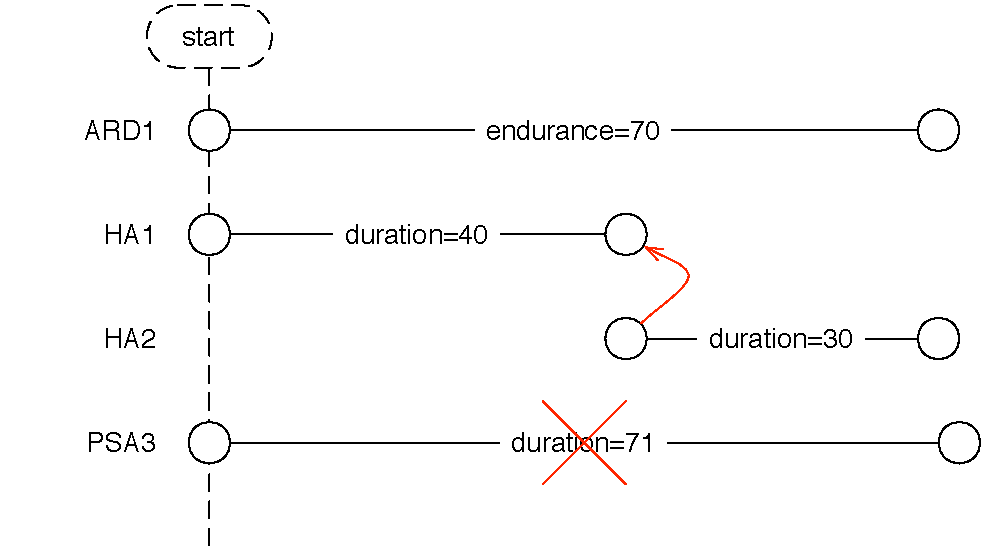
\includegraphics[scale=0.58]{img/mission-3g.pdf}
\caption[Mission 3g]{An illustration of Mission~3g, with red arrows representing preconditions and horizontal lines representing the passage of time. The \emph{x mark} denotes a point of failure for the mission.}
\label{fig:mission_3g}
\end{figure}

Finally, eight mission plans contained action workflow errors that resulted in deadlock. Figure~\ref{fig:mission_2d} illustrates this type of error with Mission~2d, which also belongs to the set of missions supporting our evaluation. Mission~2d comprises two assets with identifiers~\texttt{ARD1} and~\texttt{H1}, and three hover actions with identifiers \texttt{HA1}--\texttt{HA3}. The mission becomes deadlocked, and consequently fails, when the action workflow comprising~\texttt{HA1} and~\texttt{HA2} is disrupted. This disruption occurs because:

\begin{itemize}

\item \texttt{HA1} and~\texttt{HA2} are kinetic actions assigned to asset~\texttt{ARD1};

\item \texttt{HA1} and the cross-cutting action~\texttt{HA3}, which is assigned to asset~\texttt{H1}, are preconditions to~\texttt{HA2};

\item the duration of~\texttt{HA3} is greater than the duration of~\texttt{HA1}.

\end{itemize}

\begin{figure}[ht]
\centering
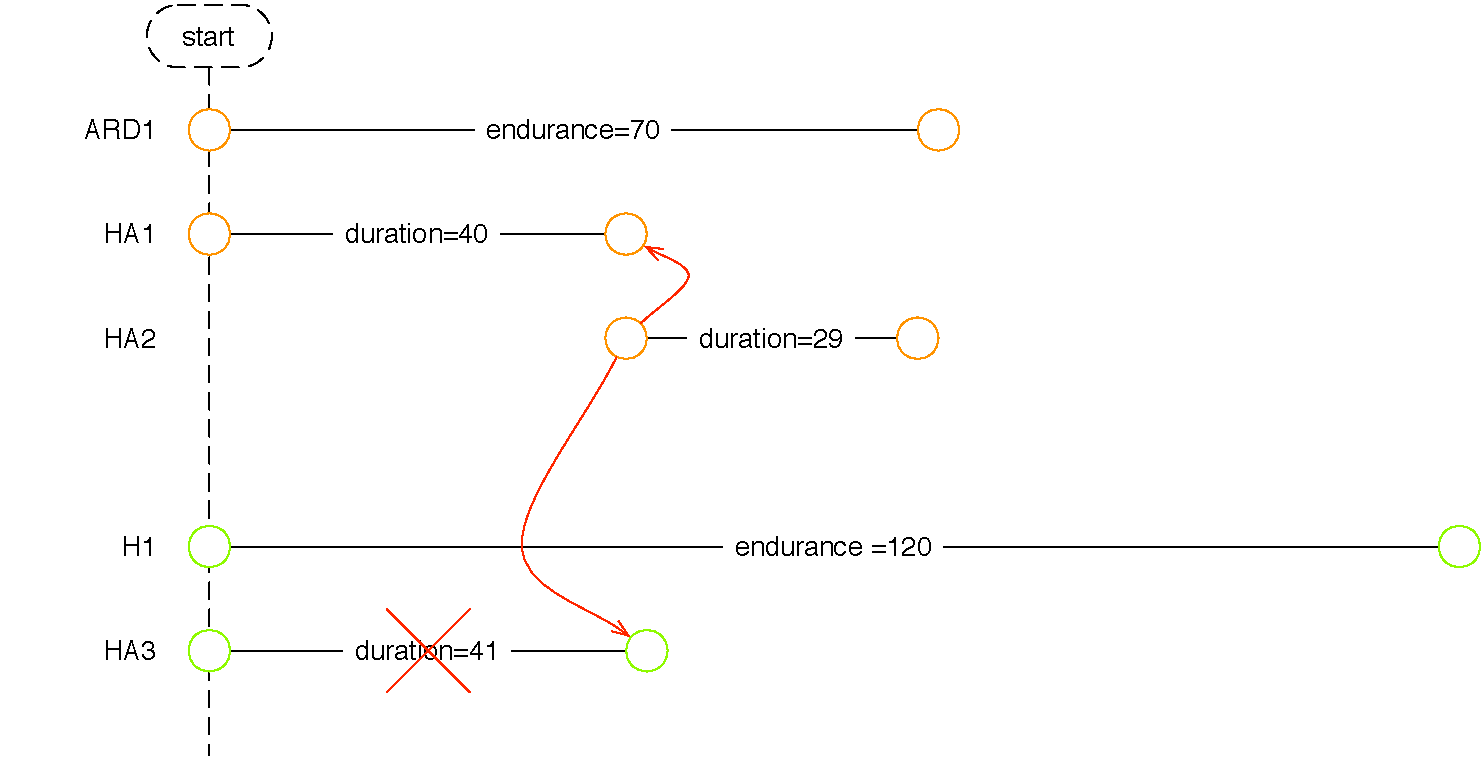
\includegraphics[scale=0.58]{img/mission-2d.pdf}
\caption[Mission 2d]{An illustration of Mission~2d, with red arrows representing preconditions and horizontal lines representing the passage of time. The \emph{x mark} denotes a point of failure for the mission. Color coded circles delineate the operation and execution of assets and actions, respectively, and group actions and the assets to which those actions are assigned.}
\label{fig:mission_2d}
\end{figure}

The propensity for cross-cutting actions to produce deadlock and thereby compromise mission correctness is associated with the degree of coupling between kinetic actions assigned to the same asset. The type of deadlock observed in Mission~2d is, to some extent, a consequence of tight coupling between the actions~\texttt{HA1} and~\texttt{HA2}, which are required by our behavioral model to execute continuously during the operation of \texttt{ARD1}. By eliminating the requirement for continuity, a looser coupling could permit~\texttt{HA2} to begin its execution after the end of~\texttt{HA3}. But missions comprising loosely coupled kinetic actions would still have to account for side effects resulting from potential workflow disruptions. For example, a loose coupling between~\texttt{HA1} and~\texttt{HA2} would enable the execution of~\texttt{HA3} to impose a hiatus on the workflow assigned to \texttt{ARD1}, with implications for the operation of that asset. We have chosen to avoid these implications, whose resolution would not have been straightforward, by establishing the deadlock in Mission~2d as a mission specification error.

The errors presented in this section were successfully identified by our prototype. While the correctness of some mission plans was absolute (with a~0.0 or~1.0 probability of success) several mission plans, including plans comprising threat area incursions, were associated with variable probabilities of success. For example, the probability of success for Mission~A is approximately~0.299 (as described in Section~\ref{sec:Synthesized_Models_and_Properties}).

\subsection{Proof of Correctness}

Given the broad range of disparate techniques described throughout this thesis, a formal proof of correctness for cascading verification may not be feasible. But correctness can be evaluated against simulations carried out during the behavioral modeling process. To this end, simulations were carried out during the development of the~58 mission plans. Simulated model executions are facilitated by the PRISM \emph{simulator}, a tool that generates sample paths through PRISM models. Partial simulation results for Mission~A are plotted by the graph in Figure~\ref{fig:mission_simulation}, where x-axis and y-axis represent variable values and time during specific executions, respectively; and plotted values represent endurance for asset~\texttt{H1} (variable~\texttt{e1}) and duration for the actions assigned to that asset (variables~\texttt{d1} and~\texttt{d2}).

\begin{figure}[ht]
\centering
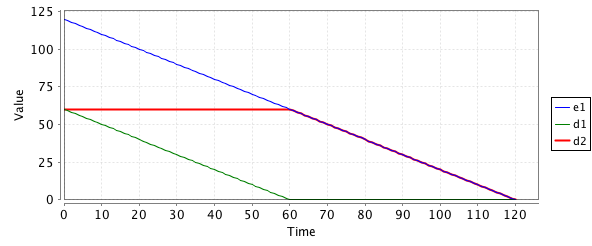
\includegraphics[width=\textwidth]{img/mission-simulation.png}
\caption[Mission simulation]{Partial simulation results for Mission~A\@. The x-axis and y-axis represent variable values and time during specific executions, respectively; and plotted values depict endurance for asset~\texttt{H1} (variable~\texttt{e1}) and duration for the actions assigned to that asset (variables~\texttt{d1} and~\texttt{d2}).}
\label{fig:mission_simulation}
\end{figure}

\section{Threats to Validity}
\label{sec:Threats_to_Validity}

This evaluation has thus far been concerned with the abstraction and effectiveness afforded by our method and prototype. Research can be evaluated further by considering threats to its validity. Threat types applicable to our research include conclusion validity, internal validity, construct validity and external validity~\cite{Wright_2010,Feldt_2010}.

Conclusion validity addresses the issue of correlation between the functionality afforded by our prototype and the correctness of UAV mission specifications, whereby correctness is determined with respect to specific properties of interest. We believe this correlation to be established by the results presented in Section~\ref{sec:Evaluation_Methods_and_Metrics}. To recap, in conjunction with the verification provided by PRISM, reduced LOC, tokens and potential (domain-specific and behavioral modeling) errors demonstrate that our method and prototype have a significant and positive effect on the correctness of UAV mission specifications.

\subsection{Internal Validity}

Having established correlation, we proceed to establish internal validity, which addresses the issue of causation between the functionality afforded by our prototype and the correctness of UAV mission specifications. For correlated variables~\emph{x} and~\emph{y}, it can be claimed that~\emph{x} causes~\emph{y} if~\emph{x} precedes~\emph{y} in the absence of \emph{confounding factors}~\cite{Seltman_2013}. We will not elaborate on the issue of precedence except to mention that our prototype's functionality precedes verification results returned by PRISM\@. The problem of confounding is somewhat more challenging.

Confounding can occur when unknown or extraneous factors affect the relationship between correlated variables. With well defined input and output interfaces, our prototype is not likely to be influenced by unknown factors. But the~58 mission plans that act as input to the prototype, and thereby generate the established correlation, could constitute an extraneous factor if they fail to 1) be grounded in the real-world, or 2) sample a sufficiently large subset of the UAV mission state space. The former concern is mitigated by the real-world mission scenarios underpinning our mission plans. The latter concern is related to the issue of variability.

We do not attempt to achieve variability with, for example, randomized mission parameters. Nevertheless, mission plans vary with respect to LOC and token values, as indicated in Table~\ref{tab:mission_metrics}. Mission plans also vary along several parameters, which are listed in Table~\ref{tab:mission_parameters} for a subset of the~58 mission plans. These parameters include numbers of assets; kinetic, sensor and cross-cutting actions; and preconditions and concurrencies. Concerns regarding the potential for mission plans to act as a confounding factor are therefore mitigated by the observed variability in both metric values and mission parameters.

\begin{table}[!ht]
	\arrayrulecolor{Gray}
	\renewcommand*\arraystretch{1.3}
	\begin{tabularx}{\textwidth}{
			>{\centering\hsize=0.08\hsize}X|
			>{\centering\hsize=0.11\hsize}X|
			>{\centering\hsize=0.11\hsize}X
			>{\centering\hsize=0.11\hsize}X
			>{\centering\hsize=0.19\hsize}X|
			>{\centering\hsize=0.2\hsize}X
			>{\centering\hsize=0.2\hsize}X
		}
		& & \multicolumn{3}{ c | }{\emph{actions}} &
				\multicolumn{2}{ c }{\emph{dependencies}}\tabularnewline
		id & assets & kinetic & sensor & cross-cutting & preconditions & concurrencies\tabularnewline
		\hline
		1a & 1 & 1 & 0 & 0 & 0 & 0 \tabularnewline
		1d & 1 & 2 & 0 & 0 & 1 & 0 \tabularnewline
		1g & 1 & 3 & 0 & 0 & 2 & 0 \tabularnewline
		2a & 2 & 3 & 0 & 0 & 1 & 0 \tabularnewline
		2b & 2 & 3 & 0 & 1 & 2 & 0 \tabularnewline
		2e & 3 & 4 & 0 & 2 & 3 & 0 \tabularnewline
		2g & 2 & 5 & 0 & 2 & 5 & 0 \tabularnewline
		2j & 2 & 5 & 0 & 1 & 4 & 0 \tabularnewline
		2m & 2 & 6 & 0 & 1 & 5 & 0 \tabularnewline
		2p & 2 & 6 & 0 & 2 & 6 & 0 \tabularnewline
		2r & 3 & 5 & 0 & 2 & 4 & 0 \tabularnewline
		2u & 3 & 6 & 0 & 2 & 5 & 0 \tabularnewline
		2v & 3 & 6 & 0 & 2 & 5 & 0 \tabularnewline
		2w & 3 & 7 & 0 & 2 & 6 & 0 \tabularnewline
		2x & 3 & 7 & 0 & 2 & 6 & 0 \tabularnewline
		3a & 1 & 1 & 1 & 0 & 0 & 0 \tabularnewline
		3e & 1 & 2 & 1 & 0 & 1 & 0 \tabularnewline
		3h & 1 & 2 & 1 & 0 & 2 & 0 \tabularnewline
		3k & 1 & 2 & 2 & 0 & 2 & 0 \tabularnewline
		3o & 1 & 2 & 2 & 0 & 3 & 0 \tabularnewline
		4a & 1 & 4 & 0 & 0 & 3 & 0 \tabularnewline
		4b & 1 & 4 & 0 & 0 & 3 & 0 \tabularnewline
		4d & 1 & 4 & 1 & 0 & 4 & 0 \tabularnewline
		4f & 1 & 4 & 2 & 0 & 5 & 0 \tabularnewline
		5a & 1 & 3 & 2 & 0 & 2 & 2 \tabularnewline
		5b & 1 & 3 & 2 & 0 & 2 & 2 \tabularnewline
	\end{tabularx}
	\caption[Mission plan parameters]{Parameters---including number of assets, actions and action dependencies---for the representative mission plans listed in Table~\ref{tab:mission_metrics}.}
	\label{tab:mission_parameters}
\end{table}

The size of DTMC and PCTL templates could constitute a second extraneous factor if PRISM-to-YAML ratios are affected by poor template design rather than the functionality afforded by our prototype. But this is not the case: our templates are not designed to create code bloat, but rather to generate PRISM code that is intelligible to a human model builder. We also note that metric values in Table~\ref{tab:mission_metrics} do not account for programmer-readable comments.

\subsection{Construct Validity}

Construct validity addresses the metrics, including LOC and token count, used to quantify model and property specification complexity. These are widely applicable, language independent software metrics that ignore logic structure and control flow. The ability to bypass control flow is useful when evaluating complexity in the context of the PRISM language, a somewhat unconventional formalism that lacks appropriate control structures.

We do acknowledge that a LOC- and token-based analysis cannot in and of itself account for the intricate syntax of the PRISM language. To address this limitation, we propose a multidimensional complexity model~\cite{Kaner_2004}, which encompasses domain-specific and behavioral modeling errors prevented by our prototype. The (potentially bidirectional) correlation between error rates and software complexity suggests that software errors can be used as descriptors of complexity~\cite{Banker_1989,Kan_2002}. By considering complexity from multiple dimensions, our metric- and error-based analysis provides a more complete understanding of PRISM artifact complexity, which in turn increases confidence in the resulting evaluation.

\subsection{External Validity}

Finally, we consider external validity, which addresses the issue of transferability/portability. In conjunction with the complexity of the UAV domain, and the real-world DARPA and DRDC mission scenarios underpinning this evaluation, the results presented in Section~\ref{sec:Evaluation_Methods_and_Metrics} suggest that cascading verification can be ported to different application domains. The portability of our method is supported by the general purpose of its constituent technologies including OWL+SWRL, Prolog, and DTMC and PCTL\@. Presently, we cannot make the same argument for the \emph{connections} that link those technologies in the context of the method. But cascading verification is an extension of semantic model checking methods with identical or comparable constituent technologies (similarities to semantic model checking were presented in Section~\ref{sec:Cascading_Verification_Related_Work}). The successful application of these methods to the Web service domain further supports the portability of cascading verification.

\section{Summary}
\label{sec:Evaluation_Summary}

By automating the synthesis of PRISM artifacts, and by providing multiple stages of reasoning and analysis, our prototype enhances the abstraction level of model and property specifications, and the effectiveness of probabilistic model checking, respectively. This cascading approach to verification improves mission correctness to a degree that is evidently unattainable by the individual components that constitute the prototype.

We note that this evaluation is preliminary. Further work is required to determine the utility of our prototype in the context of a more sophisticated mission specification language and domain model; and the ability of cascading verification to support probabilistic model checking in the context of other non-trivial domains.

\chapter{Conclusions and Future Work}
\label{chap:Conclusions_and_Future_Work}

This thesis describes a novel cascading verification method that uses composite reasoning over high-level system specifications and formalized domain knowledge to synthesize both system models and their desired behavioral properties. With cascading verification, model builders use a high-level DSL to encode system specifications that can be analyzed with model checking. Domain knowledge is encoded in OWL+SWRL and Prolog, which are combined to overcome their individual limitations. Synthesized DTMC models and PCTL properties are analyzed with the probabilistic model checker PRISM\@. Cascading verification was illustrated with a prototype system that verified the correctness of UAV mission plans. An evaluation of this prototype revealed non-trivial reductions in the size and complexity of input system specifications compared to the artifacts synthesized for PRISM\@.

The remainder of this chapter is structured as follows. Section~\ref{sec:Contributions} reiterates our contributions to the state of the art in semantic model checking. Section~\ref{sec:Future_Work} discusses directions for future work. Two specific areas of research, involving network centric and annotation-guided model checking, are described in Section~\ref{sec:Network_Centric_Model_Checking} and Section~\ref{sec:Annotation_Guided_Model_Checking}, respectively.

\section{Contributions}
\label{sec:Contributions}

With cascading verification, we claim several contributions to semantic model checking, a method that leverages semantic reasoning over domain knowledge to augment the model checking process. Unlike related work, our method synthesizes both system models \emph{and} behavioral properties for probabilistic model checking. Cascading verification is underpinned by a composite DL- and LP-based inference mechanism that overcomes expressive and reasoning limitations in the ontology language OWL\@. By using our method to verify UAV missions, we highlight the potential portability of cascading verification and, ultimately, semantic model checking, which has thus far been applied exclusively to the Web services domain.

We illustrate cascading verification with a prototype system that verifies the correctness of~58 UAV mission plans; the development of those plans is structured with DSM\@. On average, our prototype synthesizes PRISM code that is 3.127 and 4.490 times greater than the size of YAML input with regard to LOC and tokens, respectively. For traffic-surveillance missions, the prototype realizes even bigger reductions with synthesized PRISM code that is 4.522 and 8.087 times greater than the size of YAML input with regard to LOC and tokens, respectively. These results provide preliminary evidence of non-trivial reduction in the effort required to produce mission models and properties.

LOC- and token-based metrics are used to evaluate the abstraction, i.e., the reduction in modeling complexity, afforded by our prototype. In addition to enhanced abstraction, the prototype augments PRISM's verification capabilities and thereby enhances the effectiveness of probabilistic model checking. We evaluate effectiveness by presenting errors that can only be effectively eliminated with the automated synthesis of PRISM artifacts. We also evaluate the utility of the DTMC and PCTL artifacts synthesized by our prototype.

\section{Future Work}
\label{sec:Future_Work}

We have identified several promising directions for future work. Composite CVC inferences are currently unidirectional, with Prolog facts derived from knowledge encoded in OWL+SWRL\@. The effects of this \emph{pipeline} architecture were particularly pronounced in Section~\ref{sec:Classification_with_Prolog}, where semantic reasoning underpinned Prolog-based classifications, which subsequently impacted the synthesis of DTMC and PCTL artifacts. While conceptually and practically appealing, an inference pipeline constrains the reasoning process from refining Prolog inferences with ontological knowledge, and increases the potential for knowledge duplication. We aim to address these limitations by developing a knowledge representation framework that can support more flexible, iterative reasoning.

A second issue pertains to the artifacts that constitute the CVC knowledge base including CEMO, the Prolog rule-base, and the DTMC and PCTL templates. These artifacts should be extensible to reflect changes in domain knowledge. Extensions should in turn be verifiable to ensure that domain knowledge remains consistent across the entire knowledge base. This requirement provides impetus for the development of a mechanism that will automate the consistency management process.

We also intend to further the evaluation of our method and prototype by enhancing the sophistication of the mission specification language and domain model presented in this thesis. And we intend to confirm the portability of cascading verification by applying our method to other significant application domains. We expect a more robust evaluation process to facilitate the abstraction and formal specification of the connections that link different technologies in the context of our method. Once formalized, these connections will likely support the consistency management process described in the preceding paragraph, and the development of a domain-agnostic compiler. Such a compiler would receive as input the artifacts and connections that constitute a domain-specific knowledge base and thereby eliminate the current de facto requirement for bespoke implementations of the CVC\@.

Our work has yet to address the problem of tracing PRISM results back to the underlying system specifications. Without traceability, the analysis provided by PRISM may be incomprehensible to model builders~\cite{Combemale_2011}. In the context of the YAML DSL, traceability would serve to disambiguate the relationship between syntactic rules and operational semantics, which are defined with OWL and the PRISM language, respectively. Once formalized, elements of this relationship will likely parallel the connections described in the preceding paragraph.

Future work discussed thus far is closely related to the research, development, evaluation and outcomes presented in this thesis. The following sections present research directions that are more expansive in scope.

\subsection{Network-Centric Model Checking}
\label{sec:Network_Centric_Model_Checking}

Network-Centric Operations (NCO) is a doctrine that leverages information technology to improve the effectiveness and efficiency of military operations~\cite{Wilson_2007}. NCO is underpinned by contemporary socio-technological advancements, and enabled by ``a high-performance information grid, access to all appropriate information sources, weapons reach and maneuver with precision and speed of response, value-adding C2 processes---to include high-speed automated assignment of resources to need---and integrated sensor grids closely coupled in time to shooters and C2 processes.''~\cite{Cebrowski_1998} When combined, these elements support \emph{speed of command}, the process by which superior information is turned into competitive advantage. Speed of command can be substantially enhanced when command-and-control processes are automated. Enhanced speed of command accelerates the \emph{observe, orient, decide and act} (OODA) loop, which denies the enemy operational pause. Regaining this time amplifies the effects associated with speed of command, resulting in an accelerated rate of change that leads to enemy lock-out.

By automating the organization and utilization of complex operational knowledge, cascading verification could support the analysis and deployment of mission plans comprising asset configurations derived from real-time operational data including asset location, fuel and weapon statuses. Near real-time coupling of mission verification and deployment has the potential to yield a near real-time OODA loop, which will inevitably be susceptible to network and processing speed latencies. Addressing the impact of latency on mission correctness in the context of NCO constitutes an interesting research direction.

\subsection{Annotation-Guided Model Checking}
\label{sec:Annotation_Guided_Model_Checking}

With our prototype implementation of cascading verification, model builders encode mission specifications in a YAML DSL\@. Notwithstanding the inherent advantages of YAML, the introduction of a novel declarative formalism can be associated with potential disadvantages. Declarative programming that is based on first-order or higher-order logics does not cope well with temporal systems~\cite{Lloyd_1994}. This limitation, which derives from the static model theory that defines standard logics, impacts the level of expressivity afforded to mission developers. Furthermore, the novelty of our formalism increases the complexity for potential adopters, and distances the project from real-world grounding, thereby potentially compromising the utility and evaluation of our prototype.

URBI and the Robot Operating System (ROS) are sophisticated, cross-platform and open-source frameworks that support robotic software development. Both frameworks are interoperable with established programming languages, including C++ and Java, that mitigate the aforementioned limitations. With Java-encoded missions, Java annotations could be used by model builders to embed domain knowledge in executable code, and thereby guide the automated synthesis of verification artifacts. Annotation-based verification frameworks and other related work indicate this to be a promising direction for future work~\cite{Chalin_2005,Holmgren_2005,Ferreira_2007}. Development and evaluation of the proposed annotation framework would be informed by, and thereby benefit from, our experience with the existing YAML DSL\@.


\renewcommand\bibname{References}
\bibliographystyle{ieeetr}
\bibliography{bibliography}
\addcontentsline{toc}{chapter}{References}

\appendix

\chapter{Threat Area Calculations}
\label{chap:Threat_Area_Calculations}

Threat area incursions have been considered throughout this thesis. The CVC uses hard-coded geodesic equations to establish the occurrence, and calculate the duration, of threat area incursions committed by UAVs (as described in Chapter~\ref{chap:Method_Overview}). The equations employed by the CVC are underpinned by a spherical Earth with a two-dimensional surface. This rudimentary \emph{mission environment} enables our prototype to avoid complexities associated with three-dimensional topographies. (Because the shape of the Earth is approximately ellipsoidal, geodetic calculations that assume a spherical geometry result in errors ranging between 0.3\% and 0.55\%.)

In this context, a direct flightpath between two waypoints can be delineated by the minor arc of a great circle. A waypoint is a zero-dimensional spherical point designated by latitude and longitude; a great circle is the intersection of a sphere and a plane passing through the center of that sphere. The minor arc of a great circle, which we will refer to as a \emph{great circle arc}, is the shortest path between two points on the surface of a sphere.

Since great circle arcs can also be used to delineate threat area boundaries, an asset enters and exits a threat area at the intersection of two great circle arcs. We therefore use great circle intersections to establish the occurrence of threat area incursions.

\section{Establishing Threat Area Incursions}

Following from the definition of a great circle, a great circle arc lies on a plane that passes through the center of a sphere. Two great circles intersect when their respective planes intersect (the only other possibility being that the planes overlap), thereby forming a straight line that crosses the surface of the underlying sphere at two points. Consequently, the intersection of two great circle arcs must occur at one of the spherical points resulting from the intersection of the great circles underpinning those arcs.

We consider great circle arcs~\emph{a} and~\emph{b} defined by points~$a_1$, $a_2$ and~$b_1$, $b_2$, respectively. The latitude and longitude coordinates that designate these points are converted to Cartesian coordinates using Equation~\ref{eq:cartesian_coordinates}, where~\emph{R} is the Earth's mean radius (6371 kilometers).

\begin{figure}[ht]
	\begin{equation}
		\label{eq:cartesian_coordinates}
			p =
			\begin{bmatrix}
				x\\
				y\\
				z
			\end{bmatrix} =
			\begin{bmatrix}
				R \cdot \cos lat \cdot \cos lon\\
				R \cdot \cos lat \cdot \sin lon\\
				R \cdot \sin lat
			\end{bmatrix}
	\end{equation}
\end{figure}

Equation~\ref{eq:plane_vector} calculates vectors~$v_a$ and~$v_b$ from points~$a_1$, $a_2$ and~$b_1$, $b_2$, respectively, where each vector defines a plane containing the points used to calculate that vector. Equation~\ref{eq:unit_vector_a} calculates unit vectors~$u_a$ and~$u_b$ from~$v_a$ and~$v_b$, respectively. If unit vectors~$u_a$ and~$u_b$ are not identical (as determined by Equation~\ref{eq:overlaping_unit_vectors}) vectors~$v_a$ and~$v_b$ define planes that do not overlap.

\newcommand{\br}{\nonumber\\}
\newcommand{\pvlength}{\sqrt{{v_x}^2 + {v_y}^2 + {v_z}^2}}

\begin{figure}[ht]
	\begin{align}
		\label{eq:plane_vector}
			v & =
			\begin{bmatrix}
				v_x\\
				v_y\\
				v_z
			\end{bmatrix} =
			\begin{bmatrix}
				y_1 \cdot z_2 - y_2 \cdot z_1\\
				x_2 \cdot z_1 - x_1 \cdot z_2\\
				x_1 \cdot y_2 - x_2 \cdot y_1
			\end{bmatrix}\\
			\br
		\label{eq:unit_vector_a}
			u & =
			\begin{bmatrix}
				u_x\\
				u_y\\
				u_z
			\end{bmatrix} =
			\begin{bmatrix}
				v_x / \pvlength\\
				v_y / \pvlength\\
				v_z / \pvlength
			\end{bmatrix}\\
			\br
		\label{eq:overlaping_unit_vectors}
			u_1 \cap u_2 & =
			\left\{
				\begin{array}{l}
					|u_{1x} - u_{2x}| < \varepsilon\\
					|u_{1y} - u_{2y}| < \varepsilon\\
					|u_{1z} - u_{2z}| < \varepsilon
				\end{array}
			\right.
	\end{align}
\end{figure}

Two non-overlapping planes intersect in a straight line defined by direction vector~\emph{d}. Equation~\ref{eq:direction_vector} calculates~\emph{d} from vectors~$u_a$ and~$u_b$. Equation~\ref{eq:unit_vector_b} calculates the unit vector of~\emph{d}, which defines the coordinates of spherical point~$p_1$. Equation~\ref{eq:inverted_unit_vector} calculates the inverse of the unit vector of~\emph{d}, which defines the coordinates of spherical point~$p_2$. The latitude and longitude coordinates of~$p_1$ and~$p_2$ are calculated from their Cartesian coordinates using Equation~\ref{eq:latitude} and Equation~\ref{eq:longitude}, respectively. Since all values passed to trigonometric functions are expressed in radians, output from Equation~\ref{eq:latitude} and Equation~\ref{eq:longitude} must be converted from radians to degrees before proceeding to the next set of calculations.

\newcommand{\dvlength}{\sqrt{{d_x}^2 + {d_y}^2 + {d_z}^2}}

\begin{figure}[ht]
	\begin{align}
		\label{eq:direction_vector}
			d & =
			\begin{bmatrix}
				d_x\\
				d_y\\
				d_z
			\end{bmatrix} =
			\begin{bmatrix}
				u_{1y} \cdot u_{2z} - u_{2y} \cdot u_{1z}\\
				u_{2x} \cdot u_{1z} - u_{1x} \cdot u_{2z}\\
				u_{1x} \cdot u_{2y} - u_{2x} \cdot u_{1y}
			\end{bmatrix}\\
			\br
		\label{eq:unit_vector_b}
			p_1 & =
			\begin{bmatrix}
				p_{1x}\\
				p_{1y}\\
				p_{1z}
			\end{bmatrix} =
			\begin{bmatrix}
				d_x / \dvlength\\
				d_y / \dvlength\\
				d_z / \dvlength
			\end{bmatrix}\\
			\br
		\label{eq:inverted_unit_vector}
			p_2 & =
			\begin{bmatrix}
				p_{2x}\\
				p_{2y}\\
				p_{2z}
			\end{bmatrix} =
			\begin{bmatrix}
				-d_x / \dvlength\\
				-d_y / \dvlength\\
				-d_z / \dvlength
			\end{bmatrix}\\
			\br
		\label{eq:latitude}
			lat & = \arcsin \left(\frac{z}{R}\right)\\
			\br
		\label{eq:longitude}
			lon & = \arctan(y, x)
	\end{align}
\end{figure}

Having identified points~$p_1$ and~$p_2$, we check if either point is located on both arcs~\emph{a} and~\emph{b}. For arc~\emph{a} (defined by points~$a_1$ and~$a_2$) and point~$p_1$, we use the Haversine formula, which is described in Section~\ref{sec:Distance}, to calculate the distance from~$a_1$ to~$a_2$, $d_{(a_1, a_2)}$; and the distances from~$p_1$ to~$a_1$ and~$a_2$, $d_{(p_1, a_1)}$ and $d_{(p_1, a_2)}$, respectively. Consequently, $p_1 \in a \Leftrightarrow d_{(a_1, a_2)} = d_{(p_1, a_1)} + d_{(p_1, a_2)}$. Similarly, we check~$p_1$ with respect to arc~\emph{b}. If~$p_1$ is not an intersection, we check~$p_2$. If~$p_1$ and~$p_2$ are not intersection points, then arcs~\emph{a} and~\emph{b} do not intersect.

\section{Calculating Threat Area Durations}

Having established the occurrence of a threat area incursion, we proceed to calculate its duration. The duration of travel between two points is a function of distance and speed.

\subsection{Distance}
\label{sec:Distance}

A great circle distance is the shortest distance between two points along a path on the surface of a sphere. The great circle distance~\emph{d} between points~$p_1$ and~$p_2$ with coordinates $lat_1$, $lon_1$ and $lat_2$, $lon_2$, respectively, can be calculated using the Haversine formula in Equation~\ref{eq:distance}, where~\emph{R} is the Earth's mean radius~\cite{Veness}. (All values passed to trigonometric functions are assumed radians.)

\begin{figure}[ht]
	\begin{align}
		\label{eq:distance}
			\nonumber a & = \sin^2 \frac{lat_2 - lat_1}{2} + \sin^2 \frac{lon_2 - lon_1}{2} \cdot \cos lat_1 \cdot \cos lat_2\\
			\nonumber c & = 2 \cdot \arctan(\sqrt{a}, \sqrt{1 - a})\\
			d & = R \cdot c
	\end{align}
\end{figure}

\subsection{Speed}

The velocity of a UAV at any given moment during flight is a function of four parameters including the velocity of the UAV in still air; the UAV's direction of travel; and the velocity and direction of the wind. Consider a UAV with velocity vector~$v_a$, which has magnitude~$|v_a|$ and direction~$\theta_a$. The UAV flies in a wind with velocity vector~$v_w$, which has magnitude~$|v_w|$ and direction~$\theta_w$. Let~\emph{i} and ~\emph{j} be~$1 ms^{-1}$ (meters per second) East and~$1 ms^{-1}$ North, respectively. The component form for each velocity vector can be calculated using Equation~\ref{eq:UAV_velocity_vector_component_form} and Equation~\ref{eq:wind_velocity_vector_component_form}; velocity can be calculated using Equation~\ref{eq:velocity}; and the speed of the UAV in~$ms^{-1}$ can be calculated using Equation~\ref{eq:speed}.

\begin{figure}[ht]
	\begin{align}
		\label{eq:UAV_velocity_vector_component_form}
			v_a & = |v_a| \cos \theta_ai + |v_a| \sin \theta_aj\\
		\label{eq:wind_velocity_vector_component_form}
			v_w & = |v_w| \cos \theta_wi + |v_w| \sin \theta_wj\\
			\br
		\label{eq:velocity}
			v & = v_a + v_w\\
			\br
		\label{eq:speed}
			s & = |v| \approx \sqrt{{v_a}^2 + {v_w}^2}
	\end{align}
\end{figure}

\subsection{Bearing}

The direction of travel along a great circle arc is defined by initial and final bearings. The initial bearing~$\theta$ from point~$p_1$ to point~$p_2$ is calculated using Equation~\ref{eq:initial_bearing}. Because the range of~$\arctan$ is the interval $[-180^\circ, 180^\circ]$, the initial bearing is normalized to a compass bearing~$\theta_{in}$ using Equation~\ref{eq:normalized_initial_bearing}. The range of~$\theta_{in}$ is the interval $[0, 360^\circ]$. The normalized final bearing~$\theta_{fn}$ is calculated by reversing the initial bearing from~$p_2$ to~$p_1$ using Equation~\ref{eq:normalized_final_bearing}.

\begin{figure}[ht]
	\begin{align}
		\label{eq:initial_bearing}
			\nonumber y & = \sin (lon_2 - lon_1) \cdot \cos lat_2\\
			\nonumber x & = \cos lat_1 \cdot \sin lat_2 - \sin lat_1 \cdot \cos lat_2 \cdot \cos (lon_2 - lon_1)\\
			\theta & = \arctan(y, x)\\
			\br
		\label{eq:normalized_initial_bearing}
			\theta_{in} & = (\theta_{(p_1, p_2)} \cdot \frac{360}{2\pi} + 360) \bmod{360}\\
			\br
		\label{eq:normalized_final_bearing}
			\theta_{fn} & = (\theta_{(p_2, p_1)} \cdot \frac{360}{2\pi} + 180) \bmod{360}
	\end{align}
\end{figure}

Each bearing is applied to a specific route segment. The initial bearing defines the direction of travel from~$p_1$ to midpoint~$p_m$ between~$p_1$ and~$p_2$. The final bearing defines the direction of travel from~$p_m$ to~$p_2$. The latitude and longitude coordinates for~$p_m$ are calculated using Equation~\ref{eq:midpoint_latitude} and Equation~\ref{eq:midpoint_longitude}, respectively.

\begin{figure}[ht]
	\begin{align}
			\nonumber Bx & = \cos lat_2 \cdot \cos(lon_2 - lon_1)\\
			\nonumber By & = \cos lat_2 \cdot \sin(lon_2 - lon_1)\\
		\label{eq:midpoint_latitude}
			lat_m & = \arctan(\sin lat_1 + \sin lat_2, \sqrt{(\cos lat_1 + Bx)^2 + By^2})\\
		\label{eq:midpoint_longitude}
			lon_m & = lon_1 + \arctan(By, \cos lat_1 + Bx)
	\end{align}
\end{figure}

\subsection{Duration}

The duration of travel along a great circle arc defined by initial and final bearings requires calculations for two speeds and two distances. Equation~\ref{eq:extended_duration} generalizes this requirement by calculating the duration of travel along a path delineated by~\emph{n} waypoints, where $d_{(p_i, p_{i + 1})}$ is the distance in kilometers between sequential points~$p_i$ and~$p_{i + 1}$; and $s_{(p_i, p_{i + 1})}$ is the speed of travel in~$ms^{-1}$ from~$p_i$ to~$p_{i + 1}$. Because Equation~\ref{eq:distance} calculates distance in kilometers and Equation~\ref{eq:speed} calculates speed in meters per second, Equation~\ref{eq:extended_duration} converts distances to meters in order to calculate duration in seconds.

\begin{figure}[ht]
	\begin{equation}
		\label{eq:extended_duration}
			\text{duration} := \sum_{i=1}^n \frac{d_{(p_i, p_{i + 1})}}{s_{(p_i, p_{i + 1})}} \cdot 1000
	\end{equation}
\end{figure}


\singlespacing
\parskip=0em

\lstset{
	aboveskip=0em,
	basicstyle=\ttfamily\scriptsize,
	numbers=none
}

\chapter{Ontology}
\label{chap:Ontology}

\lstset{belowskip=1.8em}

\newcommand{\owlcode}[2]{\lstinputlisting[caption={OWL code for #1.},nolol=true]{src/owl/#2.txt}}

\owlcode{CEMO}{complex_missions}
\owlcode{Tactical-CEMO}{complex_tactical_missions}
\owlcode{Traffic-CEMO}{complex_traffic_surveillance_missions}
\owlcode{Mission A}{Mission_A}

\chapter{Prolog Knowledge Base}
\label{chap:Prolog_Knowledge_Base}

\lstset{belowskip=1.8em}

\newcommand{\prologlisting}[2]{\lstinputlisting[caption={Prolog code for #1.},nolol=true]{src/pl/#2.pl}}

\prologlisting{asset rules}{asset_rules}
\prologlisting{utility rules}{utility_rules}
\prologlisting{default rules}{default_rules}
\prologlisting{observer and subject rules}{observer_and_subject_rules}
\prologlisting{observer rules}{observer_rules}
\prologlisting{subject rules}{subject_rules}
\prologlisting{existential quantification rules}{existential_quantification_rules}

\chapter{PRISM Templates}
\label{chap:PRISM_Templates}

\lstset{belowskip=1.8em}

\newcommand{\rubylisting}[2]{\lstinputlisting[language=Ruby,caption={#1},nolol=true]{src/rb/#2.rb}}

\rubylisting{Ruby code for the DTMC asset module template.}{asset_template}
\rubylisting{Ruby code for the DTMC survivability template.}{survivability_template}
\rubylisting{Ruby code for the PCTL property template.}{property_template}
\rubylisting{Ruby template utility code.}{template_util}
\rubylisting{Ruby code for module \texttt{Mission}.}{mission}
\rubylisting{Ruby utility code.}{util}
\rubylisting{Ruby code for class \texttt{Asset}.}{asset}
\rubylisting{Ruby code for class \texttt{ClassLoader}.}{class_loader}
\rubylisting{Ruby code for class \texttt{HoverAction}.}{hover_action}
\rubylisting{Ruby code for class \texttt{Action}.}{action}
\rubylisting{Ruby code for class \texttt{LidarAction}.}{lidar_action}
\rubylisting{Ruby code for module \texttt{Observer}.}{observer}
\rubylisting{Ruby code for class \texttt{OpLoader}.}{op_loader}
\rubylisting{Ruby code for module \texttt{Subject}.}{subject}
\rubylisting{Code that modifies the Ruby core class \texttt{Array}.}{array}
\rubylisting{Code that modifies the Ruby core class \texttt{Hash}.}{hash}
\rubylisting{Code that modifies the Ruby core class \texttt{Module}.}{module}
\rubylisting{Code that modifies the Ruby core class \texttt{Symbol}.}{symbol}

\chapter{DSL Schema}
\label{chap:DSL_Schema}

\lstinputlisting[caption={A schema definition, encoded in the Kwalify schema language, for the YAML DSL presented in this thesis.},nolol=true]{src/yaml/schema.yaml}

\chapter{Mission Verification Artifacts}
\label{chap:Mission_Verification_Artifacts}

\lstset{belowskip=1.8em}

\newcommand{\yamllisting}[1]{
	\lstinputlisting[caption={YAML input for Mission #1.},nolol=true]{src/yaml/operation_#1.yaml}
	\lstinputlisting[caption={DTMC output for Mission #1.},nolol=true]{src/pm/operation_#1.pm}
	\lstinputlisting[caption={PCTL output for Mission #1.},nolol=true]{src/pctl/operation_#1.pctl}
	\lstinputlisting[caption={Log output for Mission #1.},nolol=true]{src/log/operation_#1.txt}
}

\yamllisting{1a}
\yamllisting{1d}
\yamllisting{1g}
\yamllisting{2a}
\yamllisting{2b}
\yamllisting{2e}
\yamllisting{2g}
\yamllisting{2j}
\yamllisting{2m}
\yamllisting{2p}
\yamllisting{2r}
\yamllisting{2u}
\yamllisting{2v}
\yamllisting{2w}
\yamllisting{2x}
\yamllisting{3a}
\yamllisting{3e}
\yamllisting{3h}
\yamllisting{3k}
\yamllisting{3o}
\yamllisting{4a}
\yamllisting{4b}
\yamllisting{4d}
\yamllisting{4f}
\yamllisting{5a}
\yamllisting{5b}


\end{document}
